\documentclass[a4paper]{book}
\usepackage{a4wide}
\usepackage{makeidx}
\usepackage{graphicx}
\usepackage{multicol}
\usepackage{float}
\usepackage{listings}
\usepackage{color}
\usepackage{textcomp}
\usepackage{alltt}
\usepackage{times}
\usepackage{ifpdf}
\ifpdf
\usepackage[pdftex,
            pagebackref=true,
            colorlinks=true,
            linkcolor=blue,
            unicode
           ]{hyperref}
\else
\usepackage[ps2pdf,
            pagebackref=true,
            colorlinks=true,
            linkcolor=blue,
            unicode
           ]{hyperref}
\usepackage{pspicture}
\fi
\usepackage[utf8]{inputenc}
\usepackage{doxygen}
\lstset{language=C++,inputencoding=utf8,basicstyle=\footnotesize,breaklines=true,breakatwhitespace=true,tabsize=4,numbers=left }
\makeindex
\setcounter{tocdepth}{3}
\renewcommand{\footrulewidth}{0.4pt}
\begin{document}
\hypersetup{pageanchor=false}
\begin{titlepage}
\vspace*{7cm}
\begin{center}
{\Large vmath \\[1ex]\large vmath-\/0.10 }\\
\vspace*{1cm}
{\large Generated by Doxygen 1.7.1}\\
\vspace*{0.5cm}
{\small Sun Nov 20 2011 20:10:09}\\
\end{center}
\end{titlepage}
\clearemptydoublepage
\pagenumbering{roman}
\tableofcontents
\clearemptydoublepage
\pagenumbering{arabic}
\hypersetup{pageanchor=true}
\chapter{Intro}
\label{index}\hypertarget{index}{}Vector mathematics for computer graphics \hypertarget{main_Features}{}\section{Features}\label{main_Features}

\begin{DoxyItemize}
\item basic arithmetic operations -\/ using operators  
\item basic linear algebra operations -\/ such as transpose, dot product, etc.  
\item aliases for vertex coordinates -\/ it means: 
\begin{DoxyPre}
  Vector3f v;
  // use vertex coordinates
  v.x = 1; v.y = 2; v.z = -1;\end{DoxyPre}



\begin{DoxyPre}  // use texture coordinates
  v.s = 0; v.t = 1; v.u = 0.5;
  // use color coordinates
  v.r = 1; v.g = 0.5; v.b = 0;
    \end{DoxyPre}
  
\item conversion constructor and assign operators -\/ so you can assign a value of \hyperlink{class_vector3}{Vector3}$<$T1$>$ type to a variable of \hyperlink{class_vector3}{Vector3}$<$T2$>$ type for any convertible T1, T2 type pairs. In other words, you can do this: 
\begin{DoxyPre}\end{DoxyPre}



\begin{DoxyPre}  Vector3f f3; Vector3d d3 = f3;
  ...
  f3 = d3;
    \end{DoxyPre}
  
\end{DoxyItemize}\hypertarget{main_Predefined}{}\section{types}\label{main_Predefined}

\begin{DoxyItemize}
\item (\hyperlink{class_vector2}{Vector2}) Two dimensional vector 
\begin{DoxyItemize}
\item float --- Vector2f 
\item double --- Vector2d 
\item int --- Vector2i 
\end{DoxyItemize}
\item (\hyperlink{class_vector3}{Vector3}) Three dimensional vector 
\begin{DoxyItemize}
\item float --- Vector3f 
\item double --- Vector3d 
\item int --- Vector3i 
\end{DoxyItemize}
\item (\hyperlink{class_vector4}{Vector4}) Four dimensional vector 
\begin{DoxyItemize}
\item float --- Vector4f 
\item double --- Vector4d 
\item int --- Vector4i 
\end{DoxyItemize}
\item (\hyperlink{class_matrix3}{Matrix3}) Matrix 3x3 
\begin{DoxyItemize}
\item float --- Matrix3f 
\item double --- Matrix3d 
\item int --- Matrix3i 
\end{DoxyItemize}
\item (\hyperlink{class_matrix4}{Matrix4}) Matrix 4x4 
\begin{DoxyItemize}
\item float --- Matrix4f 
\item double --- Matrix4d 
\item int --- Matrix4i 
\end{DoxyItemize}
\item \hyperlink{class_quaternion}{Quaternion} 
\begin{DoxyItemize}
\item float --- Quatf 
\item double --- Quatd 
\end{DoxyItemize}
\end{DoxyItemize}
\chapter{License}
\label{license}
\hypertarget{license}{}
vmath, set of classes for computer graphics mathematics.

Copyright (c) 2005-\/2011, Jan Bartipan $<$ barzto at gmail dot com $>$ All rights reserved.

Redistribution and use in source and binary forms, with or without modification, are permitted provided that the following conditions are met:


\begin{DoxyItemize}
\item Redistributions of source code must retain the above copyright notice, this list of conditions and the following disclaimer.
\item Redistributions in binary form must reproduce the above copyright notice, this list of conditions and the following disclaimer in the documentation and/or other materials provided with the distribution.
\item Neither the names of its contributors may be used to endorse or promote products derived from this software without specific prior written permission.
\end{DoxyItemize}

THIS SOFTWARE IS PROVIDED BY THE COPYRIGHT HOLDERS AND CONTRIBUTORS \char`\"{}AS IS\char`\"{} AND ANY EXPRESS OR IMPLIED WARRANTIES, INCLUDING, BUT NOT LIMITED TO, THE IMPLIED WARRANTIES OF MERCHANTABILITY AND FITNESS FOR A PARTICULAR PURPOSE ARE DISCLAIMED. IN NO EVENT SHALL THE COPYRIGHT OWNER OR CONTRIBUTORS BE LIABLE FOR ANY DIRECT, INDIRECT, INCIDENTAL, SPECIAL, EXEMPLARY, OR CONSEQUENTIAL DAMAGES (INCLUDING, BUT NOT LIMITED TO, PROCUREMENT OF SUBSTITUTE GOODS OR SERVICES; LOSS OF USE, DATA, OR PROFITS; OR BUSINESS INTERRUPTION) HOWEVER CAUSED AND ON ANY THEORY OF LIABILITY, WHETHER IN CONTRACT, STRICT LIABILITY, OR TORT (INCLUDING NEGLIGENCE OR OTHERWISE) ARISING IN ANY WAY OUT OF THE USE OF THIS SOFTWARE, EVEN IF ADVISED OF THE POSSIBILITY OF SUCH DAMAGE. 
\chapter{Class Index}
\section{Class List}
Here are the classes, structs, unions and interfaces with brief descriptions:\begin{DoxyCompactList}
\item\contentsline{section}{\hyperlink{class_matrix3}{Matrix3$<$ T $>$} (Class for matrix 3x3 )}{\pageref{class_matrix3}}{}
\item\contentsline{section}{\hyperlink{class_matrix4}{Matrix4$<$ T $>$} (Class for matrix 4x4 )}{\pageref{class_matrix4}}{}
\item\contentsline{section}{\hyperlink{class_quaternion}{Quaternion$<$ T $>$} (\hyperlink{class_quaternion}{Quaternion} class implementing some quaternion algebra operations )}{\pageref{class_quaternion}}{}
\item\contentsline{section}{\hyperlink{class_vector2}{Vector2$<$ T $>$} (Class for two dimensional vector )}{\pageref{class_vector2}}{}
\item\contentsline{section}{\hyperlink{class_vector3}{Vector3$<$ T $>$} (Class for three dimensional vector )}{\pageref{class_vector3}}{}
\item\contentsline{section}{\hyperlink{class_vector4}{Vector4$<$ T $>$} (Class for four dimensional vector )}{\pageref{class_vector4}}{}
\end{DoxyCompactList}

\chapter{File Index}
\section{File List}
Here is a list of all documented files with brief descriptions\-:\begin{DoxyCompactList}
\item\contentsline{section}{{\bfseries dirent.\-h} }{\pageref{dirent_8h}}{}
\item\contentsline{section}{{\bfseries Files.\-h} }{\pageref{_files_8h}}{}
\item\contentsline{section}{{\bfseries Jzon.\-h} }{\pageref{_jzon_8h}}{}
\item\contentsline{section}{{\bfseries Players.\-h} }{\pageref{_players_8h}}{}
\item\contentsline{section}{{\bfseries properties.\-h} }{\pageref{properties_8h}}{}
\item\contentsline{section}{\hyperlink{rules_8cpp}{rules.\-cpp} }{\pageref{rules_8cpp}}{}
\item\contentsline{section}{\hyperlink{rules_8h}{rules.\-h} }{\pageref{rules_8h}}{}
\item\contentsline{section}{{\bfseries tree.\-h} }{\pageref{tree_8h}}{}
\item\contentsline{section}{{\bfseries Units.\-h} }{\pageref{_units_8h}}{}
\item\contentsline{section}{{\bfseries Update.\-h} }{\pageref{_update_8h}}{}
\end{DoxyCompactList}

\chapter{Class Documentation}
\hypertarget{class_matrix3}{
\section{Matrix3$<$ T $>$ Class Template Reference}
\label{class_matrix3}\index{Matrix3@{Matrix3}}
}


Class for matrix 3x3.  




{\ttfamily \#include $<$vmath.h$>$}



Collaboration diagram for Matrix3$<$ T $>$:
\nopagebreak
\begin{figure}[H]
\begin{center}
\leavevmode
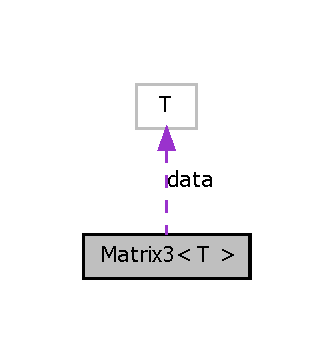
\includegraphics[width=160pt]{class_matrix3__coll__graph}
\end{center}
\end{figure}
\subsection*{Public Member Functions}
\begin{DoxyCompactItemize}
\item 
\hyperlink{class_matrix3_afbc8b655540e4b5b04d8439b606303b0}{Matrix3} ()
\begin{DoxyCompactList}\small\item\em Creates identity matrix. \item\end{DoxyCompactList}\item 
\hyperlink{class_matrix3_a3986b8f36efefb3ab2455e86fdb5e327}{Matrix3} (const T $\ast$dt)
\begin{DoxyCompactList}\small\item\em Copy matrix values from array (these data must be in column major order!). \item\end{DoxyCompactList}\item 
\hyperlink{class_matrix3_a7f0b1ceaedeffd2ab458b6dc7edc358c}{Matrix3} (const \hyperlink{class_matrix3}{Matrix3}$<$ T $>$ \&src)
\begin{DoxyCompactList}\small\item\em Copy constructor. \item\end{DoxyCompactList}\item 
{\footnotesize template$<$class FromT $>$ }\\\hyperlink{class_matrix3_acf94796374f73b4559336f08e233038c}{Matrix3} (const \hyperlink{class_matrix3}{Matrix3}$<$ FromT $>$ \&src)
\begin{DoxyCompactList}\small\item\em Copy casting constructor. \item\end{DoxyCompactList}\item 
void \hyperlink{class_matrix3_a44360e8ae549ec4b2b9c0f8ed4786761}{identity} ()
\begin{DoxyCompactList}\small\item\em Resets matrix to be identity matrix. \item\end{DoxyCompactList}\item 
bool \hyperlink{class_matrix3_acf8dc6060016d09250b8706e89f4dcc0}{operator==} (const \hyperlink{class_matrix3}{Matrix3}$<$ T $>$ \&rhs) const 
\begin{DoxyCompactList}\small\item\em Equality test operator. \item\end{DoxyCompactList}\item 
bool \hyperlink{class_matrix3_a1ecdce469f979786b1fa257a6fca3866}{operator!=} (const \hyperlink{class_matrix3}{Matrix3}$<$ T $>$ \&rhs) const 
\begin{DoxyCompactList}\small\item\em Inequality test operator. \item\end{DoxyCompactList}\item 
T \& \hyperlink{class_matrix3_aba232062fee5e35419c2c0c73aa9b88d}{at} (int x, int y)
\begin{DoxyCompactList}\small\item\em Get reference to element at position (x,y). \item\end{DoxyCompactList}\item 
const T \& \hyperlink{class_matrix3_abd32ca6519bd0131709cdeca665b4a23}{at} (int x, int y) const 
\begin{DoxyCompactList}\small\item\em Get constant reference to element at position (x,y). \item\end{DoxyCompactList}\item 
T \& \hyperlink{class_matrix3_a21a0e224becfb4fa4447d4c656ad3d0c}{operator()} (int i, int j)
\begin{DoxyCompactList}\small\item\em Get reference to element at position (i,j), with math matrix notation. \item\end{DoxyCompactList}\item 
const T \& \hyperlink{class_matrix3_a345b3ea5baef035e1272506540c2905c}{operator()} (int i, int j) const 
\begin{DoxyCompactList}\small\item\em Get constant reference to element at position (i,j), with math matrix notation. \item\end{DoxyCompactList}\item 
\hyperlink{class_matrix3}{Matrix3}$<$ T $>$ \& \hyperlink{class_matrix3_afcd3742e1bb4ce693fd28c751a4d8e9c}{operator=} (const \hyperlink{class_matrix3}{Matrix3}$<$ T $>$ \&rhs)
\begin{DoxyCompactList}\small\item\em Copy operator. \item\end{DoxyCompactList}\item 
{\footnotesize template$<$class FromT $>$ }\\\hyperlink{class_matrix3}{Matrix3}$<$ T $>$ \& \hyperlink{class_matrix3_a8fc1aae99bf569de84249e8716ce50e8}{operator=} (const \hyperlink{class_matrix3}{Matrix3}$<$ FromT $>$ \&rhs)
\begin{DoxyCompactList}\small\item\em Copy casting operator. \item\end{DoxyCompactList}\item 
\hyperlink{class_matrix3}{Matrix3}$<$ T $>$ \& \hyperlink{class_matrix3_a0c34f193be3802cae81c4cbfdfab1a53}{operator=} (const T $\ast$rhs)
\begin{DoxyCompactList}\small\item\em Copy operator. \item\end{DoxyCompactList}\item 
\hyperlink{class_matrix3}{Matrix3}$<$ T $>$ \hyperlink{class_matrix3_ad960991a64a1e6c72e21c29fb8c1f890}{operator+} (const \hyperlink{class_matrix3}{Matrix3}$<$ T $>$ \&rhs) const 
\begin{DoxyCompactList}\small\item\em Addition operator. \item\end{DoxyCompactList}\item 
\hyperlink{class_matrix3}{Matrix3}$<$ T $>$ \hyperlink{class_matrix3_aeb5ca229fa633ceec14fc93fa873234d}{operator-\/} (const \hyperlink{class_matrix3}{Matrix3}$<$ T $>$ \&rhs) const 
\begin{DoxyCompactList}\small\item\em Subtraction operator. \item\end{DoxyCompactList}\item 
\hyperlink{class_matrix3}{Matrix3}$<$ T $>$ \hyperlink{class_matrix3_a635803865b0b5c3c0e2102a44d7ed5d8}{operator+} (T rhs) const 
\begin{DoxyCompactList}\small\item\em Addition operator. \item\end{DoxyCompactList}\item 
\hyperlink{class_matrix3}{Matrix3}$<$ T $>$ \hyperlink{class_matrix3_a708ee4b7775f551c63e1d1820ef1d7b2}{operator-\/} (T rhs) const 
\begin{DoxyCompactList}\small\item\em Subtraction operator. \item\end{DoxyCompactList}\item 
\hyperlink{class_matrix3}{Matrix3}$<$ T $>$ \hyperlink{class_matrix3_a4a7053f22eee3c50ef099181983370c9}{operator$\ast$} (T rhs) const 
\begin{DoxyCompactList}\small\item\em Multiplication operator. \item\end{DoxyCompactList}\item 
\hyperlink{class_matrix3}{Matrix3}$<$ T $>$ \hyperlink{class_matrix3_abf53af4ad067516b153c76a9e18cc410}{operator/} (T rhs) const 
\begin{DoxyCompactList}\small\item\em Division operator. \item\end{DoxyCompactList}\item 
\hyperlink{class_vector3}{Vector3}$<$ T $>$ \hyperlink{class_matrix3_add25a42745c41871b2d3b808f0d5047e}{operator$\ast$} (const \hyperlink{class_vector3}{Vector3}$<$ T $>$ \&rhs) const 
\begin{DoxyCompactList}\small\item\em Multiplication operator. \item\end{DoxyCompactList}\item 
\hyperlink{class_matrix3}{Matrix3}$<$ T $>$ \hyperlink{class_matrix3_abd84667793375507dc98fc8e896d89b3}{operator$\ast$} (\hyperlink{class_matrix3}{Matrix3}$<$ T $>$ rhs) const 
\begin{DoxyCompactList}\small\item\em Multiplication operator. \item\end{DoxyCompactList}\item 
\hyperlink{class_matrix3}{Matrix3}$<$ T $>$ \hyperlink{class_matrix3_aafac87a5bb5afd70a7a8b39257f28558}{transpose} ()
\begin{DoxyCompactList}\small\item\em Transpose matrix. \item\end{DoxyCompactList}\item 
\hyperlink{class_matrix3}{Matrix3}$<$ T $>$ \hyperlink{class_matrix3_a3c16292eeaf2514a4fc26de912cf07e0}{lerp} (T fact, const \hyperlink{class_matrix3}{Matrix3}$<$ T $>$ \&rhs) const 
\begin{DoxyCompactList}\small\item\em Linear interpolation of two matrices. \item\end{DoxyCompactList}\item 
T \hyperlink{class_matrix3_a4cba34533d0f88feb8a622e5c5b7052d}{det} ()
\item 
\hyperlink{class_matrix3}{Matrix3}$<$ T $>$ \hyperlink{class_matrix3_aad3810622196a42d5f1a58e7d49d1417}{inverse} ()
\begin{DoxyCompactList}\small\item\em Computes inverse matrix. \item\end{DoxyCompactList}\item 
\hyperlink{class_matrix3_a643aecc11c95f9706a7620deab32a4ee}{operator T $\ast$} ()
\begin{DoxyCompactList}\small\item\em Conversion to pointer operator. \item\end{DoxyCompactList}\item 
\hyperlink{class_matrix3_a103a13ad3c2c32985e6e10adb91088f2}{operator const T $\ast$} () const 
\begin{DoxyCompactList}\small\item\em Conversion to pointer operator. \item\end{DoxyCompactList}\item 
std::string \hyperlink{class_matrix3_a4208a1713fc7fb654a88eb7b82ef3b02}{toString} () const 
\begin{DoxyCompactList}\small\item\em Gets string representation. \item\end{DoxyCompactList}\end{DoxyCompactItemize}
\subsection*{Static Public Member Functions}
\begin{DoxyCompactItemize}
\item 
static \hyperlink{class_matrix3}{Matrix3}$<$ T $>$ \hyperlink{class_matrix3_a1e39496a1d1708ddc1658b0bf2f448f2}{createRotationAroundAxis} (T xDeg, T yDeg, T zDeg)
\begin{DoxyCompactList}\small\item\em Creates rotation matrix by rotation around axis. \item\end{DoxyCompactList}\item 
{\footnotesize template$<$class It $>$ }\\static \hyperlink{class_matrix3}{Matrix3}$<$ T $>$ \hyperlink{class_matrix3_af183cabaf18b9922fd11e517c5cf26b1}{fromOde} (const It $\ast$mat)
\begin{DoxyCompactList}\small\item\em Creates rotation matrix from ODE Matrix. \item\end{DoxyCompactList}\item 
{\footnotesize template$<$class FromT $>$ }\\static \hyperlink{class_matrix3}{Matrix3}$<$ T $>$ \hyperlink{class_matrix3_abce4ed104a81e64ce9cbd479f0105625}{fromRowMajorArray} (const FromT $\ast$arr)
\begin{DoxyCompactList}\small\item\em Creates new matrix 3x3 from array that represents such matrix 3x3 as array of tightly packed elements in row major order. \item\end{DoxyCompactList}\item 
{\footnotesize template$<$class FromT $>$ }\\static \hyperlink{class_matrix3}{Matrix3}$<$ T $>$ \hyperlink{class_matrix3_a54ac5b79264837228f219067e92aa853}{fromColumnMajorArray} (const FromT $\ast$arr)
\begin{DoxyCompactList}\small\item\em Creates new matrix 3x3 from array that represents such matrix 3x3 as array of tightly packed elements in column major order. \item\end{DoxyCompactList}\end{DoxyCompactItemize}
\subsection*{Public Attributes}
\begin{DoxyCompactItemize}
\item 
T \hyperlink{class_matrix3_ad0e5ea83502126b24d468ae8cc67255d}{data} \mbox{[}9\mbox{]}
\begin{DoxyCompactList}\small\item\em Data stored in column major order. \item\end{DoxyCompactList}\end{DoxyCompactItemize}
\subsection*{Friends}
\begin{DoxyCompactItemize}
\item 
std::ostream \& \hyperlink{class_matrix3_a281742a1b77b4a4bf76ac03f7b75ee74}{operator$<$$<$} (std::ostream \&lhs, const \hyperlink{class_matrix3}{Matrix3}$<$ T $>$ \&rhs)
\begin{DoxyCompactList}\small\item\em Output to stream operator. \item\end{DoxyCompactList}\end{DoxyCompactItemize}


\subsection{Detailed Description}
\subsubsection*{template$<$class T$>$ class Matrix3$<$ T $>$}

Class for matrix 3x3. \begin{DoxyNote}{Note}
Data stored in this matrix are in column major order. This arrangement suits OpenGL. If you're using row major matrix, consider using fromRowMajorArray as way for construction Matrix3$<$T$>$ instance. 
\end{DoxyNote}


\subsection{Constructor \& Destructor Documentation}
\hypertarget{class_matrix3_afbc8b655540e4b5b04d8439b606303b0}{
\index{Matrix3@{Matrix3}!Matrix3@{Matrix3}}
\index{Matrix3@{Matrix3}!Matrix3@{Matrix3}}
\subsubsection[{Matrix3}]{\setlength{\rightskip}{0pt plus 5cm}template$<$class T$>$ {\bf Matrix3}$<$ T $>$::{\bf Matrix3} (
\begin{DoxyParamCaption}
{}
\end{DoxyParamCaption}
)\hspace{0.3cm}{\ttfamily  \mbox{[}inline\mbox{]}}}}
\label{class_matrix3_afbc8b655540e4b5b04d8439b606303b0}


Creates identity matrix. 

\hypertarget{class_matrix3_a3986b8f36efefb3ab2455e86fdb5e327}{
\index{Matrix3@{Matrix3}!Matrix3@{Matrix3}}
\index{Matrix3@{Matrix3}!Matrix3@{Matrix3}}
\subsubsection[{Matrix3}]{\setlength{\rightskip}{0pt plus 5cm}template$<$class T$>$ {\bf Matrix3}$<$ T $>$::{\bf Matrix3} (
\begin{DoxyParamCaption}
\item[{const T $\ast$}]{ dt}
\end{DoxyParamCaption}
)\hspace{0.3cm}{\ttfamily  \mbox{[}inline\mbox{]}}}}
\label{class_matrix3_a3986b8f36efefb3ab2455e86fdb5e327}


Copy matrix values from array (these data must be in column major order!). 

\hypertarget{class_matrix3_a7f0b1ceaedeffd2ab458b6dc7edc358c}{
\index{Matrix3@{Matrix3}!Matrix3@{Matrix3}}
\index{Matrix3@{Matrix3}!Matrix3@{Matrix3}}
\subsubsection[{Matrix3}]{\setlength{\rightskip}{0pt plus 5cm}template$<$class T$>$ {\bf Matrix3}$<$ T $>$::{\bf Matrix3} (
\begin{DoxyParamCaption}
\item[{const {\bf Matrix3}$<$ T $>$ \&}]{ src}
\end{DoxyParamCaption}
)\hspace{0.3cm}{\ttfamily  \mbox{[}inline\mbox{]}}}}
\label{class_matrix3_a7f0b1ceaedeffd2ab458b6dc7edc358c}


Copy constructor. 


\begin{DoxyParams}{Parameters}
\item[{\em src}]Data source for new created instance of \hyperlink{class_matrix3}{Matrix3} \end{DoxyParams}
\hypertarget{class_matrix3_acf94796374f73b4559336f08e233038c}{
\index{Matrix3@{Matrix3}!Matrix3@{Matrix3}}
\index{Matrix3@{Matrix3}!Matrix3@{Matrix3}}
\subsubsection[{Matrix3}]{\setlength{\rightskip}{0pt plus 5cm}template$<$class T$>$ template$<$class FromT $>$ {\bf Matrix3}$<$ T $>$::{\bf Matrix3} (
\begin{DoxyParamCaption}
\item[{const {\bf Matrix3}$<$ FromT $>$ \&}]{ src}
\end{DoxyParamCaption}
)\hspace{0.3cm}{\ttfamily  \mbox{[}inline\mbox{]}}}}
\label{class_matrix3_acf94796374f73b4559336f08e233038c}


Copy casting constructor. 


\begin{DoxyParams}{Parameters}
\item[{\em src}]Data source for new created instance of \hyperlink{class_matrix3}{Matrix3} \end{DoxyParams}


\subsection{Member Function Documentation}
\hypertarget{class_matrix3_aba232062fee5e35419c2c0c73aa9b88d}{
\index{Matrix3@{Matrix3}!at@{at}}
\index{at@{at}!Matrix3@{Matrix3}}
\subsubsection[{at}]{\setlength{\rightskip}{0pt plus 5cm}template$<$class T$>$ T\& {\bf Matrix3}$<$ T $>$::at (
\begin{DoxyParamCaption}
\item[{int}]{ x, }
\item[{int}]{ y}
\end{DoxyParamCaption}
)\hspace{0.3cm}{\ttfamily  \mbox{[}inline\mbox{]}}}}
\label{class_matrix3_aba232062fee5e35419c2c0c73aa9b88d}


Get reference to element at position (x,y). 


\begin{DoxyParams}{Parameters}
\item[{\em x}]Number of column (0..2) \item[{\em y}]Number of row (0..2) \end{DoxyParams}
\hypertarget{class_matrix3_abd32ca6519bd0131709cdeca665b4a23}{
\index{Matrix3@{Matrix3}!at@{at}}
\index{at@{at}!Matrix3@{Matrix3}}
\subsubsection[{at}]{\setlength{\rightskip}{0pt plus 5cm}template$<$class T$>$ const T\& {\bf Matrix3}$<$ T $>$::at (
\begin{DoxyParamCaption}
\item[{int}]{ x, }
\item[{int}]{ y}
\end{DoxyParamCaption}
) const\hspace{0.3cm}{\ttfamily  \mbox{[}inline\mbox{]}}}}
\label{class_matrix3_abd32ca6519bd0131709cdeca665b4a23}


Get constant reference to element at position (x,y). 


\begin{DoxyParams}{Parameters}
\item[{\em x}]Number of column (0..2) \item[{\em y}]Number of row (0..2) \end{DoxyParams}
\hypertarget{class_matrix3_a1e39496a1d1708ddc1658b0bf2f448f2}{
\index{Matrix3@{Matrix3}!createRotationAroundAxis@{createRotationAroundAxis}}
\index{createRotationAroundAxis@{createRotationAroundAxis}!Matrix3@{Matrix3}}
\subsubsection[{createRotationAroundAxis}]{\setlength{\rightskip}{0pt plus 5cm}template$<$class T$>$ static {\bf Matrix3}$<$T$>$ {\bf Matrix3}$<$ T $>$::createRotationAroundAxis (
\begin{DoxyParamCaption}
\item[{T}]{ xDeg, }
\item[{T}]{ yDeg, }
\item[{T}]{ zDeg}
\end{DoxyParamCaption}
)\hspace{0.3cm}{\ttfamily  \mbox{[}inline, static\mbox{]}}}}
\label{class_matrix3_a1e39496a1d1708ddc1658b0bf2f448f2}


Creates rotation matrix by rotation around axis. 


\begin{DoxyParams}{Parameters}
\item[{\em xDeg}]Angle (in degrees) of rotation around axis X. \item[{\em yDeg}]Angle (in degrees) of rotation around axis Y. \item[{\em zDeg}]Angle (in degrees) of rotation around axis Z. \end{DoxyParams}
\hypertarget{class_matrix3_a4cba34533d0f88feb8a622e5c5b7052d}{
\index{Matrix3@{Matrix3}!det@{det}}
\index{det@{det}!Matrix3@{Matrix3}}
\subsubsection[{det}]{\setlength{\rightskip}{0pt plus 5cm}template$<$class T$>$ T {\bf Matrix3}$<$ T $>$::det (
\begin{DoxyParamCaption}
{}
\end{DoxyParamCaption}
)\hspace{0.3cm}{\ttfamily  \mbox{[}inline\mbox{]}}}}
\label{class_matrix3_a4cba34533d0f88feb8a622e5c5b7052d}
\hypertarget{class_matrix3_a54ac5b79264837228f219067e92aa853}{
\index{Matrix3@{Matrix3}!fromColumnMajorArray@{fromColumnMajorArray}}
\index{fromColumnMajorArray@{fromColumnMajorArray}!Matrix3@{Matrix3}}
\subsubsection[{fromColumnMajorArray}]{\setlength{\rightskip}{0pt plus 5cm}template$<$class T$>$ template$<$class FromT $>$ static {\bf Matrix3}$<$T$>$ {\bf Matrix3}$<$ T $>$::fromColumnMajorArray (
\begin{DoxyParamCaption}
\item[{const FromT $\ast$}]{ arr}
\end{DoxyParamCaption}
)\hspace{0.3cm}{\ttfamily  \mbox{[}inline, static\mbox{]}}}}
\label{class_matrix3_a54ac5b79264837228f219067e92aa853}


Creates new matrix 3x3 from array that represents such matrix 3x3 as array of tightly packed elements in column major order. 


\begin{DoxyParams}{Parameters}
\item[{\em arr}]An array of elements for 3x3 matrix in column major order. \end{DoxyParams}
\begin{DoxyReturn}{Returns}
An instance of Matrix3$<$T$>$ representing {\itshape arr\/} 
\end{DoxyReturn}
\hypertarget{class_matrix3_af183cabaf18b9922fd11e517c5cf26b1}{
\index{Matrix3@{Matrix3}!fromOde@{fromOde}}
\index{fromOde@{fromOde}!Matrix3@{Matrix3}}
\subsubsection[{fromOde}]{\setlength{\rightskip}{0pt plus 5cm}template$<$class T$>$ template$<$class It $>$ static {\bf Matrix3}$<$T$>$ {\bf Matrix3}$<$ T $>$::fromOde (
\begin{DoxyParamCaption}
\item[{const It $\ast$}]{ mat}
\end{DoxyParamCaption}
)\hspace{0.3cm}{\ttfamily  \mbox{[}inline, static\mbox{]}}}}
\label{class_matrix3_af183cabaf18b9922fd11e517c5cf26b1}


Creates rotation matrix from ODE Matrix. 

\hypertarget{class_matrix3_abce4ed104a81e64ce9cbd479f0105625}{
\index{Matrix3@{Matrix3}!fromRowMajorArray@{fromRowMajorArray}}
\index{fromRowMajorArray@{fromRowMajorArray}!Matrix3@{Matrix3}}
\subsubsection[{fromRowMajorArray}]{\setlength{\rightskip}{0pt plus 5cm}template$<$class T$>$ template$<$class FromT $>$ static {\bf Matrix3}$<$T$>$ {\bf Matrix3}$<$ T $>$::fromRowMajorArray (
\begin{DoxyParamCaption}
\item[{const FromT $\ast$}]{ arr}
\end{DoxyParamCaption}
)\hspace{0.3cm}{\ttfamily  \mbox{[}inline, static\mbox{]}}}}
\label{class_matrix3_abce4ed104a81e64ce9cbd479f0105625}


Creates new matrix 3x3 from array that represents such matrix 3x3 as array of tightly packed elements in row major order. 


\begin{DoxyParams}{Parameters}
\item[{\em arr}]An array of elements for 3x3 matrix in row major order. \end{DoxyParams}
\begin{DoxyReturn}{Returns}
An instance of Matrix3$<$T$>$ representing {\itshape arr\/} 
\end{DoxyReturn}
\hypertarget{class_matrix3_a44360e8ae549ec4b2b9c0f8ed4786761}{
\index{Matrix3@{Matrix3}!identity@{identity}}
\index{identity@{identity}!Matrix3@{Matrix3}}
\subsubsection[{identity}]{\setlength{\rightskip}{0pt plus 5cm}template$<$class T$>$ void {\bf Matrix3}$<$ T $>$::identity (
\begin{DoxyParamCaption}
{}
\end{DoxyParamCaption}
)\hspace{0.3cm}{\ttfamily  \mbox{[}inline\mbox{]}}}}
\label{class_matrix3_a44360e8ae549ec4b2b9c0f8ed4786761}


Resets matrix to be identity matrix. 

\hypertarget{class_matrix3_aad3810622196a42d5f1a58e7d49d1417}{
\index{Matrix3@{Matrix3}!inverse@{inverse}}
\index{inverse@{inverse}!Matrix3@{Matrix3}}
\subsubsection[{inverse}]{\setlength{\rightskip}{0pt plus 5cm}template$<$class T$>$ {\bf Matrix3}$<$T$>$ {\bf Matrix3}$<$ T $>$::inverse (
\begin{DoxyParamCaption}
{}
\end{DoxyParamCaption}
)\hspace{0.3cm}{\ttfamily  \mbox{[}inline\mbox{]}}}}
\label{class_matrix3_aad3810622196a42d5f1a58e7d49d1417}


Computes inverse matrix. 

\begin{DoxyReturn}{Returns}
Inverse matrix of this matrix. 
\end{DoxyReturn}
\hypertarget{class_matrix3_a3c16292eeaf2514a4fc26de912cf07e0}{
\index{Matrix3@{Matrix3}!lerp@{lerp}}
\index{lerp@{lerp}!Matrix3@{Matrix3}}
\subsubsection[{lerp}]{\setlength{\rightskip}{0pt plus 5cm}template$<$class T$>$ {\bf Matrix3}$<$T$>$ {\bf Matrix3}$<$ T $>$::lerp (
\begin{DoxyParamCaption}
\item[{T}]{ fact, }
\item[{const {\bf Matrix3}$<$ T $>$ \&}]{ rhs}
\end{DoxyParamCaption}
) const\hspace{0.3cm}{\ttfamily  \mbox{[}inline\mbox{]}}}}
\label{class_matrix3_a3c16292eeaf2514a4fc26de912cf07e0}


Linear interpolation of two matrices. 


\begin{DoxyParams}{Parameters}
\item[{\em fact}]Factor of interpolation. For translation from positon of this matrix (lhs) to matrix rhs, values of factor goes from 0.0 to 1.0. \item[{\em rhs}]Second Matrix for interpolation \end{DoxyParams}
\begin{DoxyNote}{Note}
However values of fact parameter are reasonable only in interval \mbox{[}0.0 , 1.0\mbox{]}, you can pass also values outside of this interval and you can get result (extrapolation?) 
\end{DoxyNote}
\hypertarget{class_matrix3_a103a13ad3c2c32985e6e10adb91088f2}{
\index{Matrix3@{Matrix3}!operator const T $\ast$@{operator const T $\ast$}}
\index{operator const T $\ast$@{operator const T $\ast$}!Matrix3@{Matrix3}}
\subsubsection[{operator const T $\ast$}]{\setlength{\rightskip}{0pt plus 5cm}template$<$class T$>$ {\bf Matrix3}$<$ T $>$::operator const T $\ast$ (
\begin{DoxyParamCaption}
{}
\end{DoxyParamCaption}
) const\hspace{0.3cm}{\ttfamily  \mbox{[}inline\mbox{]}}}}
\label{class_matrix3_a103a13ad3c2c32985e6e10adb91088f2}


Conversion to pointer operator. 

\begin{DoxyReturn}{Returns}
Constant Pointer to internally stored (in management of class Matrix3$<$T$>$) used for passing Matrix3$<$T$>$ values to gl$\ast$\mbox{[}fd\mbox{]}v functions. 
\end{DoxyReturn}
\hypertarget{class_matrix3_a643aecc11c95f9706a7620deab32a4ee}{
\index{Matrix3@{Matrix3}!operator T $\ast$@{operator T $\ast$}}
\index{operator T $\ast$@{operator T $\ast$}!Matrix3@{Matrix3}}
\subsubsection[{operator T $\ast$}]{\setlength{\rightskip}{0pt plus 5cm}template$<$class T$>$ {\bf Matrix3}$<$ T $>$::operator T $\ast$ (
\begin{DoxyParamCaption}
{}
\end{DoxyParamCaption}
)\hspace{0.3cm}{\ttfamily  \mbox{[}inline\mbox{]}}}}
\label{class_matrix3_a643aecc11c95f9706a7620deab32a4ee}


Conversion to pointer operator. 

\begin{DoxyReturn}{Returns}
Pointer to internally stored (in management of class Matrix3$<$T$>$) used for passing Matrix3$<$T$>$ values to gl$\ast$\mbox{[}fd\mbox{]}v functions. 
\end{DoxyReturn}
\hypertarget{class_matrix3_a1ecdce469f979786b1fa257a6fca3866}{
\index{Matrix3@{Matrix3}!operator!=@{operator!=}}
\index{operator!=@{operator!=}!Matrix3@{Matrix3}}
\subsubsection[{operator!=}]{\setlength{\rightskip}{0pt plus 5cm}template$<$class T$>$ bool {\bf Matrix3}$<$ T $>$::operator!= (
\begin{DoxyParamCaption}
\item[{const {\bf Matrix3}$<$ T $>$ \&}]{ rhs}
\end{DoxyParamCaption}
) const\hspace{0.3cm}{\ttfamily  \mbox{[}inline\mbox{]}}}}
\label{class_matrix3_a1ecdce469f979786b1fa257a6fca3866}


Inequality test operator. 


\begin{DoxyParams}{Parameters}
\item[{\em rhs}]Right hand side argument of binary operator. \end{DoxyParams}
\begin{DoxyReturn}{Returns}
not (lhs == rhs) :-\/P 
\end{DoxyReturn}
\hypertarget{class_matrix3_a21a0e224becfb4fa4447d4c656ad3d0c}{
\index{Matrix3@{Matrix3}!operator()@{operator()}}
\index{operator()@{operator()}!Matrix3@{Matrix3}}
\subsubsection[{operator()}]{\setlength{\rightskip}{0pt plus 5cm}template$<$class T$>$ T\& {\bf Matrix3}$<$ T $>$::operator() (
\begin{DoxyParamCaption}
\item[{int}]{ i, }
\item[{int}]{ j}
\end{DoxyParamCaption}
)\hspace{0.3cm}{\ttfamily  \mbox{[}inline\mbox{]}}}}
\label{class_matrix3_a21a0e224becfb4fa4447d4c656ad3d0c}


Get reference to element at position (i,j), with math matrix notation. 


\begin{DoxyParams}{Parameters}
\item[{\em i}]Number of row (1..3) \item[{\em j}]Number of column (1..3) \end{DoxyParams}
\hypertarget{class_matrix3_a345b3ea5baef035e1272506540c2905c}{
\index{Matrix3@{Matrix3}!operator()@{operator()}}
\index{operator()@{operator()}!Matrix3@{Matrix3}}
\subsubsection[{operator()}]{\setlength{\rightskip}{0pt plus 5cm}template$<$class T$>$ const T\& {\bf Matrix3}$<$ T $>$::operator() (
\begin{DoxyParamCaption}
\item[{int}]{ i, }
\item[{int}]{ j}
\end{DoxyParamCaption}
) const\hspace{0.3cm}{\ttfamily  \mbox{[}inline\mbox{]}}}}
\label{class_matrix3_a345b3ea5baef035e1272506540c2905c}


Get constant reference to element at position (i,j), with math matrix notation. 


\begin{DoxyParams}{Parameters}
\item[{\em i}]Number of row (1..3) \item[{\em j}]Number of column (1..3) \end{DoxyParams}
\hypertarget{class_matrix3_a4a7053f22eee3c50ef099181983370c9}{
\index{Matrix3@{Matrix3}!operator$\ast$@{operator$\ast$}}
\index{operator$\ast$@{operator$\ast$}!Matrix3@{Matrix3}}
\subsubsection[{operator$\ast$}]{\setlength{\rightskip}{0pt plus 5cm}template$<$class T$>$ {\bf Matrix3}$<$T$>$ {\bf Matrix3}$<$ T $>$::operator$\ast$ (
\begin{DoxyParamCaption}
\item[{T}]{ rhs}
\end{DoxyParamCaption}
) const\hspace{0.3cm}{\ttfamily  \mbox{[}inline\mbox{]}}}}
\label{class_matrix3_a4a7053f22eee3c50ef099181983370c9}


Multiplication operator. 


\begin{DoxyParams}{Parameters}
\item[{\em rhs}]Right hand side argument of binary operator. \end{DoxyParams}
\hypertarget{class_matrix3_add25a42745c41871b2d3b808f0d5047e}{
\index{Matrix3@{Matrix3}!operator$\ast$@{operator$\ast$}}
\index{operator$\ast$@{operator$\ast$}!Matrix3@{Matrix3}}
\subsubsection[{operator$\ast$}]{\setlength{\rightskip}{0pt plus 5cm}template$<$class T$>$ {\bf Vector3}$<$T$>$ {\bf Matrix3}$<$ T $>$::operator$\ast$ (
\begin{DoxyParamCaption}
\item[{const {\bf Vector3}$<$ T $>$ \&}]{ rhs}
\end{DoxyParamCaption}
) const\hspace{0.3cm}{\ttfamily  \mbox{[}inline\mbox{]}}}}
\label{class_matrix3_add25a42745c41871b2d3b808f0d5047e}


Multiplication operator. 


\begin{DoxyParams}{Parameters}
\item[{\em rhs}]Right hand side argument of binary operator. \end{DoxyParams}
\hypertarget{class_matrix3_abd84667793375507dc98fc8e896d89b3}{
\index{Matrix3@{Matrix3}!operator$\ast$@{operator$\ast$}}
\index{operator$\ast$@{operator$\ast$}!Matrix3@{Matrix3}}
\subsubsection[{operator$\ast$}]{\setlength{\rightskip}{0pt plus 5cm}template$<$class T$>$ {\bf Matrix3}$<$T$>$ {\bf Matrix3}$<$ T $>$::operator$\ast$ (
\begin{DoxyParamCaption}
\item[{{\bf Matrix3}$<$ T $>$}]{ rhs}
\end{DoxyParamCaption}
) const\hspace{0.3cm}{\ttfamily  \mbox{[}inline\mbox{]}}}}
\label{class_matrix3_abd84667793375507dc98fc8e896d89b3}


Multiplication operator. 


\begin{DoxyParams}{Parameters}
\item[{\em rhs}]Right hand side argument of binary operator. \end{DoxyParams}
\hypertarget{class_matrix3_a635803865b0b5c3c0e2102a44d7ed5d8}{
\index{Matrix3@{Matrix3}!operator+@{operator+}}
\index{operator+@{operator+}!Matrix3@{Matrix3}}
\subsubsection[{operator+}]{\setlength{\rightskip}{0pt plus 5cm}template$<$class T$>$ {\bf Matrix3}$<$T$>$ {\bf Matrix3}$<$ T $>$::operator+ (
\begin{DoxyParamCaption}
\item[{T}]{ rhs}
\end{DoxyParamCaption}
) const\hspace{0.3cm}{\ttfamily  \mbox{[}inline\mbox{]}}}}
\label{class_matrix3_a635803865b0b5c3c0e2102a44d7ed5d8}


Addition operator. 


\begin{DoxyParams}{Parameters}
\item[{\em rhs}]Right hand side argument of binary operator. \end{DoxyParams}
\hypertarget{class_matrix3_ad960991a64a1e6c72e21c29fb8c1f890}{
\index{Matrix3@{Matrix3}!operator+@{operator+}}
\index{operator+@{operator+}!Matrix3@{Matrix3}}
\subsubsection[{operator+}]{\setlength{\rightskip}{0pt plus 5cm}template$<$class T$>$ {\bf Matrix3}$<$T$>$ {\bf Matrix3}$<$ T $>$::operator+ (
\begin{DoxyParamCaption}
\item[{const {\bf Matrix3}$<$ T $>$ \&}]{ rhs}
\end{DoxyParamCaption}
) const\hspace{0.3cm}{\ttfamily  \mbox{[}inline\mbox{]}}}}
\label{class_matrix3_ad960991a64a1e6c72e21c29fb8c1f890}


Addition operator. 


\begin{DoxyParams}{Parameters}
\item[{\em rhs}]Right hand side argument of binary operator. \end{DoxyParams}
\hypertarget{class_matrix3_aeb5ca229fa633ceec14fc93fa873234d}{
\index{Matrix3@{Matrix3}!operator-\/@{operator-\/}}
\index{operator-\/@{operator-\/}!Matrix3@{Matrix3}}
\subsubsection[{operator-\/}]{\setlength{\rightskip}{0pt plus 5cm}template$<$class T$>$ {\bf Matrix3}$<$T$>$ {\bf Matrix3}$<$ T $>$::operator-\/ (
\begin{DoxyParamCaption}
\item[{const {\bf Matrix3}$<$ T $>$ \&}]{ rhs}
\end{DoxyParamCaption}
) const\hspace{0.3cm}{\ttfamily  \mbox{[}inline\mbox{]}}}}
\label{class_matrix3_aeb5ca229fa633ceec14fc93fa873234d}


Subtraction operator. 


\begin{DoxyParams}{Parameters}
\item[{\em rhs}]Right hand side argument of binary operator. \end{DoxyParams}
\hypertarget{class_matrix3_a708ee4b7775f551c63e1d1820ef1d7b2}{
\index{Matrix3@{Matrix3}!operator-\/@{operator-\/}}
\index{operator-\/@{operator-\/}!Matrix3@{Matrix3}}
\subsubsection[{operator-\/}]{\setlength{\rightskip}{0pt plus 5cm}template$<$class T$>$ {\bf Matrix3}$<$T$>$ {\bf Matrix3}$<$ T $>$::operator-\/ (
\begin{DoxyParamCaption}
\item[{T}]{ rhs}
\end{DoxyParamCaption}
) const\hspace{0.3cm}{\ttfamily  \mbox{[}inline\mbox{]}}}}
\label{class_matrix3_a708ee4b7775f551c63e1d1820ef1d7b2}


Subtraction operator. 


\begin{DoxyParams}{Parameters}
\item[{\em rhs}]Right hand side argument of binary operator. \end{DoxyParams}
\hypertarget{class_matrix3_abf53af4ad067516b153c76a9e18cc410}{
\index{Matrix3@{Matrix3}!operator/@{operator/}}
\index{operator/@{operator/}!Matrix3@{Matrix3}}
\subsubsection[{operator/}]{\setlength{\rightskip}{0pt plus 5cm}template$<$class T$>$ {\bf Matrix3}$<$T$>$ {\bf Matrix3}$<$ T $>$::operator/ (
\begin{DoxyParamCaption}
\item[{T}]{ rhs}
\end{DoxyParamCaption}
) const\hspace{0.3cm}{\ttfamily  \mbox{[}inline\mbox{]}}}}
\label{class_matrix3_abf53af4ad067516b153c76a9e18cc410}


Division operator. 


\begin{DoxyParams}{Parameters}
\item[{\em rhs}]Right hand side argument of binary operator. \end{DoxyParams}
\hypertarget{class_matrix3_afcd3742e1bb4ce693fd28c751a4d8e9c}{
\index{Matrix3@{Matrix3}!operator=@{operator=}}
\index{operator=@{operator=}!Matrix3@{Matrix3}}
\subsubsection[{operator=}]{\setlength{\rightskip}{0pt plus 5cm}template$<$class T$>$ {\bf Matrix3}$<$T$>$\& {\bf Matrix3}$<$ T $>$::operator= (
\begin{DoxyParamCaption}
\item[{const {\bf Matrix3}$<$ T $>$ \&}]{ rhs}
\end{DoxyParamCaption}
)\hspace{0.3cm}{\ttfamily  \mbox{[}inline\mbox{]}}}}
\label{class_matrix3_afcd3742e1bb4ce693fd28c751a4d8e9c}


Copy operator. 


\begin{DoxyParams}{Parameters}
\item[{\em rhs}]Right hand side argument of binary operator. \end{DoxyParams}
\hypertarget{class_matrix3_a0c34f193be3802cae81c4cbfdfab1a53}{
\index{Matrix3@{Matrix3}!operator=@{operator=}}
\index{operator=@{operator=}!Matrix3@{Matrix3}}
\subsubsection[{operator=}]{\setlength{\rightskip}{0pt plus 5cm}template$<$class T$>$ {\bf Matrix3}$<$T$>$\& {\bf Matrix3}$<$ T $>$::operator= (
\begin{DoxyParamCaption}
\item[{const T $\ast$}]{ rhs}
\end{DoxyParamCaption}
)\hspace{0.3cm}{\ttfamily  \mbox{[}inline\mbox{]}}}}
\label{class_matrix3_a0c34f193be3802cae81c4cbfdfab1a53}


Copy operator. 


\begin{DoxyParams}{Parameters}
\item[{\em rhs}]Right hand side argument of binary operator. \end{DoxyParams}
\hypertarget{class_matrix3_a8fc1aae99bf569de84249e8716ce50e8}{
\index{Matrix3@{Matrix3}!operator=@{operator=}}
\index{operator=@{operator=}!Matrix3@{Matrix3}}
\subsubsection[{operator=}]{\setlength{\rightskip}{0pt plus 5cm}template$<$class T$>$ template$<$class FromT $>$ {\bf Matrix3}$<$T$>$\& {\bf Matrix3}$<$ T $>$::operator= (
\begin{DoxyParamCaption}
\item[{const {\bf Matrix3}$<$ FromT $>$ \&}]{ rhs}
\end{DoxyParamCaption}
)\hspace{0.3cm}{\ttfamily  \mbox{[}inline\mbox{]}}}}
\label{class_matrix3_a8fc1aae99bf569de84249e8716ce50e8}


Copy casting operator. 


\begin{DoxyParams}{Parameters}
\item[{\em rhs}]Right hand side argument of binary operator. \end{DoxyParams}
\hypertarget{class_matrix3_acf8dc6060016d09250b8706e89f4dcc0}{
\index{Matrix3@{Matrix3}!operator==@{operator==}}
\index{operator==@{operator==}!Matrix3@{Matrix3}}
\subsubsection[{operator==}]{\setlength{\rightskip}{0pt plus 5cm}template$<$class T$>$ bool {\bf Matrix3}$<$ T $>$::operator== (
\begin{DoxyParamCaption}
\item[{const {\bf Matrix3}$<$ T $>$ \&}]{ rhs}
\end{DoxyParamCaption}
) const\hspace{0.3cm}{\ttfamily  \mbox{[}inline\mbox{]}}}}
\label{class_matrix3_acf8dc6060016d09250b8706e89f4dcc0}


Equality test operator. 


\begin{DoxyParams}{Parameters}
\item[{\em rhs}]Right hand side argument of binary operator. \end{DoxyParams}
\begin{DoxyNote}{Note}
Test of equality is based of threshold EPSILON value. To be two values equal, must satisfy this condition all elements of matrix $|$ lhs\mbox{[}i\mbox{]} -\/ rhs\mbox{[}i\mbox{]} $|$ $<$ EPSILON, same for y-\/coordinate, z-\/coordinate, and w-\/coordinate. 
\end{DoxyNote}
\hypertarget{class_matrix3_a4208a1713fc7fb654a88eb7b82ef3b02}{
\index{Matrix3@{Matrix3}!toString@{toString}}
\index{toString@{toString}!Matrix3@{Matrix3}}
\subsubsection[{toString}]{\setlength{\rightskip}{0pt plus 5cm}template$<$class T$>$ std::string {\bf Matrix3}$<$ T $>$::toString (
\begin{DoxyParamCaption}
{}
\end{DoxyParamCaption}
) const\hspace{0.3cm}{\ttfamily  \mbox{[}inline\mbox{]}}}}
\label{class_matrix3_a4208a1713fc7fb654a88eb7b82ef3b02}


Gets string representation. 

\hypertarget{class_matrix3_aafac87a5bb5afd70a7a8b39257f28558}{
\index{Matrix3@{Matrix3}!transpose@{transpose}}
\index{transpose@{transpose}!Matrix3@{Matrix3}}
\subsubsection[{transpose}]{\setlength{\rightskip}{0pt plus 5cm}template$<$class T$>$ {\bf Matrix3}$<$T$>$ {\bf Matrix3}$<$ T $>$::transpose (
\begin{DoxyParamCaption}
{}
\end{DoxyParamCaption}
)\hspace{0.3cm}{\ttfamily  \mbox{[}inline\mbox{]}}}}
\label{class_matrix3_aafac87a5bb5afd70a7a8b39257f28558}


Transpose matrix. 



\subsection{Friends And Related Function Documentation}
\hypertarget{class_matrix3_a281742a1b77b4a4bf76ac03f7b75ee74}{
\index{Matrix3@{Matrix3}!operator$<$$<$@{operator$<$$<$}}
\index{operator$<$$<$@{operator$<$$<$}!Matrix3@{Matrix3}}
\subsubsection[{operator$<$$<$}]{\setlength{\rightskip}{0pt plus 5cm}template$<$class T$>$ std::ostream\& operator$<$$<$ (
\begin{DoxyParamCaption}
\item[{std::ostream \&}]{ lhs, }
\item[{const {\bf Matrix3}$<$ T $>$ \&}]{ rhs}
\end{DoxyParamCaption}
)\hspace{0.3cm}{\ttfamily  \mbox{[}friend\mbox{]}}}}
\label{class_matrix3_a281742a1b77b4a4bf76ac03f7b75ee74}


Output to stream operator. 


\begin{DoxyParams}{Parameters}
\item[{\em lhs}]Left hand side argument of operator (commonly ostream instance). \item[{\em rhs}]Right hand side argument of operator. \end{DoxyParams}
\begin{DoxyReturn}{Returns}
Left hand side argument -\/ the ostream object passed to operator. 
\end{DoxyReturn}


\subsection{Member Data Documentation}
\hypertarget{class_matrix3_ad0e5ea83502126b24d468ae8cc67255d}{
\index{Matrix3@{Matrix3}!data@{data}}
\index{data@{data}!Matrix3@{Matrix3}}
\subsubsection[{data}]{\setlength{\rightskip}{0pt plus 5cm}template$<$class T$>$ T {\bf Matrix3}$<$ T $>$::{\bf data}\mbox{[}9\mbox{]}}}
\label{class_matrix3_ad0e5ea83502126b24d468ae8cc67255d}


Data stored in column major order. 



The documentation for this class was generated from the following file:\begin{DoxyCompactItemize}
\item 
src/\hyperlink{vmath_8h}{vmath.h}\end{DoxyCompactItemize}

\hypertarget{class_matrix4}{
\section{Matrix4$<$ T $>$ Class Template Reference}
\label{class_matrix4}\index{Matrix4@{Matrix4}}
}


Class for matrix 4x4.  




{\ttfamily \#include $<$vmath.h$>$}



Collaboration diagram for Matrix4$<$ T $>$:
\nopagebreak
\begin{figure}[H]
\begin{center}
\leavevmode
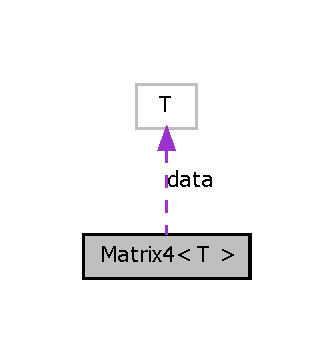
\includegraphics[width=160pt]{class_matrix4__coll__graph}
\end{center}
\end{figure}
\subsection*{Public Member Functions}
\begin{DoxyCompactItemize}
\item 
\hyperlink{class_matrix4_ab24760b5fdf4cac34df976d6820394c2}{Matrix4} ()
\begin{DoxyCompactList}\small\item\em Creates identity matrix. \item\end{DoxyCompactList}\item 
\hyperlink{class_matrix4_a49ad707e9df6e90d71b4e1ee631340fd}{Matrix4} (const T $\ast$dt)
\begin{DoxyCompactList}\small\item\em Copy matrix values from array (these data must be in column major order!). \item\end{DoxyCompactList}\item 
\hyperlink{class_matrix4_a222824e031d77fea24ef41d30a4b0e4a}{Matrix4} (const \hyperlink{class_matrix4}{Matrix4}$<$ T $>$ \&src)
\begin{DoxyCompactList}\small\item\em Copy constructor. \item\end{DoxyCompactList}\item 
{\footnotesize template$<$class FromT $>$ }\\\hyperlink{class_matrix4_a55afc9a90ad770fba8043b20f5c744d5}{Matrix4} (const \hyperlink{class_matrix4}{Matrix4}$<$ FromT $>$ \&src)
\begin{DoxyCompactList}\small\item\em Copy casting constructor. \item\end{DoxyCompactList}\item 
void \hyperlink{class_matrix4_a0477c32b08c8d45ca1cc1b99026c34e9}{identity} ()
\begin{DoxyCompactList}\small\item\em Resets matrix to be identity matrix. \item\end{DoxyCompactList}\item 
bool \hyperlink{class_matrix4_a35c2d2ba0451091b51d4e2b10bee24ae}{operator==} (const \hyperlink{class_matrix4}{Matrix4}$<$ T $>$ \&rhs) const 
\begin{DoxyCompactList}\small\item\em Equality test operator. \item\end{DoxyCompactList}\item 
bool \hyperlink{class_matrix4_a8558057b529d2441c3812bb37fe2c7c0}{operator!=} (const \hyperlink{class_matrix4}{Matrix4}$<$ T $>$ \&rhs) const 
\begin{DoxyCompactList}\small\item\em Inequality test operator. \item\end{DoxyCompactList}\item 
T \& \hyperlink{class_matrix4_a81152afb471fe9b150dba7b427d01555}{at} (int x, int y)
\begin{DoxyCompactList}\small\item\em Get reference to element at postion (x,y). \item\end{DoxyCompactList}\item 
const T \& \hyperlink{class_matrix4_a849f6ec28740c645f666501e49d2afd4}{at} (int x, int y) const 
\begin{DoxyCompactList}\small\item\em Get constant reference to element at position (x,y). \item\end{DoxyCompactList}\item 
T \& \hyperlink{class_matrix4_abcb2856588551e655f80da7c88e7c33e}{operator()} (int i, int j)
\begin{DoxyCompactList}\small\item\em Get reference to element at position (i,j), with math matrix notation. \item\end{DoxyCompactList}\item 
const T \& \hyperlink{class_matrix4_ad6b68f514be803e215ca967f9d5dc55c}{operator()} (int i, int j) const 
\begin{DoxyCompactList}\small\item\em Get constant reference to element at position (i,j), with math matrix notation. \item\end{DoxyCompactList}\item 
void \hyperlink{class_matrix4_ab6e5ff74b76ccabddb0109da608fdf04}{setTranslation} (const \hyperlink{class_vector3}{Vector3}$<$ T $>$ \&v)
\begin{DoxyCompactList}\small\item\em Sets translation part of matrix. \item\end{DoxyCompactList}\item 
\hyperlink{class_vector3}{Vector3}$<$ T $>$ \hyperlink{class_matrix4_a9c89b73d65fa5a0544efcf26829d8b5e}{getTranslation} ()
\item 
void \hyperlink{class_matrix4_a1364b4ea9ddb21af98db5256f82a0515}{setRotation} (const \hyperlink{class_matrix3}{Matrix3}$<$ T $>$ \&m)
\begin{DoxyCompactList}\small\item\em Sets rotation part (matrix 3x3) of matrix. \item\end{DoxyCompactList}\item 
\hyperlink{class_matrix4}{Matrix4}$<$ T $>$ \& \hyperlink{class_matrix4_abaab668421b08bb7588f5e41a508099c}{operator=} (const \hyperlink{class_matrix4}{Matrix4}$<$ T $>$ \&rhs)
\begin{DoxyCompactList}\small\item\em Copy operator. \item\end{DoxyCompactList}\item 
{\footnotesize template$<$class FromT $>$ }\\\hyperlink{class_matrix4}{Matrix4}$<$ T $>$ \& \hyperlink{class_matrix4_a7100801643261624c02ce196185a3436}{operator=} (const \hyperlink{class_matrix4}{Matrix4}$<$ FromT $>$ \&rhs)
\begin{DoxyCompactList}\small\item\em Copy casting operator. \item\end{DoxyCompactList}\item 
\hyperlink{class_matrix4}{Matrix4}$<$ T $>$ \& \hyperlink{class_matrix4_a180ee55d24b911aa98b6d30f4824ddec}{operator=} (const T $\ast$rhs)
\begin{DoxyCompactList}\small\item\em Copy operator. \item\end{DoxyCompactList}\item 
\hyperlink{class_matrix4}{Matrix4}$<$ T $>$ \hyperlink{class_matrix4_a114856c2bd8e47908c40cbd6d18533f1}{operator+} (const \hyperlink{class_matrix4}{Matrix4}$<$ T $>$ \&rhs) const 
\begin{DoxyCompactList}\small\item\em Addition operator. \item\end{DoxyCompactList}\item 
\hyperlink{class_matrix4}{Matrix4}$<$ T $>$ \hyperlink{class_matrix4_a385f1a4401e78842e8061fe350f74540}{operator-\/} (const \hyperlink{class_matrix4}{Matrix4}$<$ T $>$ \&rhs) const 
\begin{DoxyCompactList}\small\item\em Subtraction operator. \item\end{DoxyCompactList}\item 
\hyperlink{class_matrix4}{Matrix4}$<$ T $>$ \hyperlink{class_matrix4_a5b7adc0c653a4c261f563d9a4ad9a095}{operator+} (T rhs) const 
\begin{DoxyCompactList}\small\item\em Addition operator. \item\end{DoxyCompactList}\item 
\hyperlink{class_matrix4}{Matrix4}$<$ T $>$ \hyperlink{class_matrix4_aa8aa96061eba82c08bac660b75ce46b1}{operator-\/} (T rhs) const 
\begin{DoxyCompactList}\small\item\em Subtraction operator. \item\end{DoxyCompactList}\item 
\hyperlink{class_matrix4}{Matrix4}$<$ T $>$ \hyperlink{class_matrix4_ade719cd04adda7472e087c665546df47}{operator$\ast$} (T rhs) const 
\begin{DoxyCompactList}\small\item\em Multiplication operator. \item\end{DoxyCompactList}\item 
\hyperlink{class_matrix4}{Matrix4}$<$ T $>$ \hyperlink{class_matrix4_a2048ef268e7a5ddc6c10dc2ec7952962}{operator/} (T rhs) const 
\begin{DoxyCompactList}\small\item\em Division operator. \item\end{DoxyCompactList}\item 
\hyperlink{class_vector4}{Vector4}$<$ T $>$ \hyperlink{class_matrix4_adc1e42ef0b1606d6824f44d5ad87f23c}{operator$\ast$} (const \hyperlink{class_vector4}{Vector4}$<$ T $>$ \&rhs) const 
\begin{DoxyCompactList}\small\item\em Multiplication operator. \item\end{DoxyCompactList}\item 
\hyperlink{class_vector3}{Vector3}$<$ T $>$ \hyperlink{class_matrix4_aaf6ce02d773283e544fd781abaa1ab5c}{operator$\ast$} (const \hyperlink{class_vector3}{Vector3}$<$ T $>$ \&rhs) const 
\begin{DoxyCompactList}\small\item\em Multiplication operator. \item\end{DoxyCompactList}\item 
\hyperlink{class_matrix4}{Matrix4}$<$ T $>$ \hyperlink{class_matrix4_afe91d8df25ea2a6b631cbcb288996c5d}{operator$\ast$} (\hyperlink{class_matrix4}{Matrix4}$<$ T $>$ rhs) const 
\begin{DoxyCompactList}\small\item\em Multiplication operator. \item\end{DoxyCompactList}\item 
T \hyperlink{class_matrix4_a1c124a69945d5913abff0a17990f17d0}{det} ()
\begin{DoxyCompactList}\small\item\em Computes determinant of matrix. \item\end{DoxyCompactList}\item 
\hyperlink{class_matrix4}{Matrix4}$<$ T $>$ \hyperlink{class_matrix4_a8412458379c9a664437d74e6a1a28443}{inverse} ()
\begin{DoxyCompactList}\small\item\em Computes inverse matrix. \item\end{DoxyCompactList}\item 
\hyperlink{class_matrix4}{Matrix4}$<$ T $>$ \hyperlink{class_matrix4_af58e316035425ba563a23e3b8f53c73c}{transpose} ()
\begin{DoxyCompactList}\small\item\em Transpose matrix. \item\end{DoxyCompactList}\item 
\hyperlink{class_matrix4}{Matrix4}$<$ T $>$ \hyperlink{class_matrix4_a0d895fccd560d767e9b6c672b806d8f5}{lerp} (T fact, const \hyperlink{class_matrix4}{Matrix4}$<$ T $>$ \&rhs) const 
\begin{DoxyCompactList}\small\item\em Linear interpolation of two matrices. \item\end{DoxyCompactList}\item 
\hyperlink{class_matrix4_aaac5f73c7974eee0056d4e4379d6465a}{operator T $\ast$} ()
\begin{DoxyCompactList}\small\item\em Conversion to pointer operator. \item\end{DoxyCompactList}\item 
\hyperlink{class_matrix4_acd9956981d8c1a19a003373893520ca5}{operator const T $\ast$} () const 
\begin{DoxyCompactList}\small\item\em Conversion to pointer operator. \item\end{DoxyCompactList}\item 
std::string \hyperlink{class_matrix4_a1121fd84f7636290ae1e2fb7ac6c6c9c}{toString} () const 
\begin{DoxyCompactList}\small\item\em Gets string representation. \item\end{DoxyCompactList}\end{DoxyCompactItemize}
\subsection*{Static Public Member Functions}
\begin{DoxyCompactItemize}
\item 
static \hyperlink{class_matrix4}{Matrix4}$<$ T $>$ \hyperlink{class_matrix4_a55c7865b25c33d0b02835a8ac8d32db8}{createRotationAroundAxis} (T xDeg, T yDeg, T zDeg)
\begin{DoxyCompactList}\small\item\em Creates rotation matrix by rotation around axis. \item\end{DoxyCompactList}\item 
static \hyperlink{class_matrix4}{Matrix4}$<$ T $>$ \hyperlink{class_matrix4_a7b68a758485c1f5b8239ed7632658519}{createTranslation} (T x, T y, T z, T w=1)
\begin{DoxyCompactList}\small\item\em Creates translation matrix. \item\end{DoxyCompactList}\item 
static \hyperlink{class_matrix4}{Matrix4}$<$ T $>$ \hyperlink{class_matrix4_a0b8035f3d1144444d6835cd60642009d}{createLookAt} (const \hyperlink{class_vector3}{Vector3}$<$ T $>$ \&eyePos, const \hyperlink{class_vector3}{Vector3}$<$ T $>$ \&centerPos, const \hyperlink{class_vector3}{Vector3}$<$ T $>$ \&upDir)
\begin{DoxyCompactList}\small\item\em Creates new view matrix to look from specified position {\itshape eyePos\/} to specified position {\itshape centerPos\/}. \item\end{DoxyCompactList}\item 
static \hyperlink{class_matrix4}{Matrix4}$<$ T $>$ \hyperlink{class_matrix4_a3874c4332bb5f89a03eac10641ad9f06}{createFrustum} (T left, T right, T bottom, T top, T zNear, T zFar)
\begin{DoxyCompactList}\small\item\em Creates OpenGL compatible perspective projection according specified frustum parameters. \item\end{DoxyCompactList}\item 
static \hyperlink{class_matrix4}{Matrix4}$<$ T $>$ \hyperlink{class_matrix4_af678671e87d2fafd79fe8b00344f2229}{createOrtho} (T left, T right, T bottom, T top, T zNear, T zFar)
\begin{DoxyCompactList}\small\item\em Creates OpenGL compatible orthographic projection matrix. \item\end{DoxyCompactList}\item 
{\footnotesize template$<$class FromT $>$ }\\static \hyperlink{class_matrix4}{Matrix4}$<$ T $>$ \hyperlink{class_matrix4_af5d6a66cc20b3558b448104099d9693e}{fromRowMajorArray} (const FromT $\ast$arr)
\begin{DoxyCompactList}\small\item\em Creates new matrix 4x4 from array that represents such matrix 4x4 as array of tightly packed elements in row major order. \item\end{DoxyCompactList}\item 
{\footnotesize template$<$class FromT $>$ }\\static \hyperlink{class_matrix4}{Matrix4}$<$ T $>$ \hyperlink{class_matrix4_a1c9e68efd1cd024385403a57fcacf513}{fromColumnMajorArray} (const FromT $\ast$arr)
\begin{DoxyCompactList}\small\item\em Creates new matrix 4x4 from array that represents such matrix 4x4 as array of tightly packed elements in column major order. \item\end{DoxyCompactList}\end{DoxyCompactItemize}
\subsection*{Public Attributes}
\begin{DoxyCompactItemize}
\item 
T \hyperlink{class_matrix4_a8941190ba31803101cdfd94ff89f2a66}{data} \mbox{[}16\mbox{]}
\begin{DoxyCompactList}\small\item\em Data stored in column major order. \item\end{DoxyCompactList}\end{DoxyCompactItemize}
\subsection*{Friends}
\begin{DoxyCompactItemize}
\item 
std::ostream \& \hyperlink{class_matrix4_a0c80b0aa66b23ac6ad3bdcf81a0ada10}{operator$<$$<$} (std::ostream \&lhs, const \hyperlink{class_matrix4}{Matrix4}$<$ T $>$ \&rhs)
\begin{DoxyCompactList}\small\item\em Output to stream operator. \item\end{DoxyCompactList}\end{DoxyCompactItemize}


\subsection{Detailed Description}
\subsubsection*{template$<$class T$>$ class Matrix4$<$ T $>$}

Class for matrix 4x4. \begin{DoxyNote}{Note}
Data stored in this matrix are in column major order. This arrangement suits OpenGL. If you're using row major matrix, consider using fromRowMajorArray as way for construction Matrix4$<$T$>$ instance. 
\end{DoxyNote}


\subsection{Constructor \& Destructor Documentation}
\hypertarget{class_matrix4_ab24760b5fdf4cac34df976d6820394c2}{
\index{Matrix4@{Matrix4}!Matrix4@{Matrix4}}
\index{Matrix4@{Matrix4}!Matrix4@{Matrix4}}
\subsubsection[{Matrix4}]{\setlength{\rightskip}{0pt plus 5cm}template$<$class T$>$ {\bf Matrix4}$<$ T $>$::{\bf Matrix4} (
\begin{DoxyParamCaption}
{}
\end{DoxyParamCaption}
)\hspace{0.3cm}{\ttfamily  \mbox{[}inline\mbox{]}}}}
\label{class_matrix4_ab24760b5fdf4cac34df976d6820394c2}


Creates identity matrix. 

\hypertarget{class_matrix4_a49ad707e9df6e90d71b4e1ee631340fd}{
\index{Matrix4@{Matrix4}!Matrix4@{Matrix4}}
\index{Matrix4@{Matrix4}!Matrix4@{Matrix4}}
\subsubsection[{Matrix4}]{\setlength{\rightskip}{0pt plus 5cm}template$<$class T$>$ {\bf Matrix4}$<$ T $>$::{\bf Matrix4} (
\begin{DoxyParamCaption}
\item[{const T $\ast$}]{ dt}
\end{DoxyParamCaption}
)\hspace{0.3cm}{\ttfamily  \mbox{[}inline\mbox{]}}}}
\label{class_matrix4_a49ad707e9df6e90d71b4e1ee631340fd}


Copy matrix values from array (these data must be in column major order!). 

\hypertarget{class_matrix4_a222824e031d77fea24ef41d30a4b0e4a}{
\index{Matrix4@{Matrix4}!Matrix4@{Matrix4}}
\index{Matrix4@{Matrix4}!Matrix4@{Matrix4}}
\subsubsection[{Matrix4}]{\setlength{\rightskip}{0pt plus 5cm}template$<$class T$>$ {\bf Matrix4}$<$ T $>$::{\bf Matrix4} (
\begin{DoxyParamCaption}
\item[{const {\bf Matrix4}$<$ T $>$ \&}]{ src}
\end{DoxyParamCaption}
)\hspace{0.3cm}{\ttfamily  \mbox{[}inline\mbox{]}}}}
\label{class_matrix4_a222824e031d77fea24ef41d30a4b0e4a}


Copy constructor. 


\begin{DoxyParams}{Parameters}
\item[{\em src}]Data source for new created instance of \hyperlink{class_matrix4}{Matrix4}. \end{DoxyParams}
\hypertarget{class_matrix4_a55afc9a90ad770fba8043b20f5c744d5}{
\index{Matrix4@{Matrix4}!Matrix4@{Matrix4}}
\index{Matrix4@{Matrix4}!Matrix4@{Matrix4}}
\subsubsection[{Matrix4}]{\setlength{\rightskip}{0pt plus 5cm}template$<$class T$>$ template$<$class FromT $>$ {\bf Matrix4}$<$ T $>$::{\bf Matrix4} (
\begin{DoxyParamCaption}
\item[{const {\bf Matrix4}$<$ FromT $>$ \&}]{ src}
\end{DoxyParamCaption}
)\hspace{0.3cm}{\ttfamily  \mbox{[}inline\mbox{]}}}}
\label{class_matrix4_a55afc9a90ad770fba8043b20f5c744d5}


Copy casting constructor. 


\begin{DoxyParams}{Parameters}
\item[{\em src}]Data source for new created instance of \hyperlink{class_matrix4}{Matrix4}. \end{DoxyParams}


\subsection{Member Function Documentation}
\hypertarget{class_matrix4_a81152afb471fe9b150dba7b427d01555}{
\index{Matrix4@{Matrix4}!at@{at}}
\index{at@{at}!Matrix4@{Matrix4}}
\subsubsection[{at}]{\setlength{\rightskip}{0pt plus 5cm}template$<$class T$>$ T\& {\bf Matrix4}$<$ T $>$::at (
\begin{DoxyParamCaption}
\item[{int}]{ x, }
\item[{int}]{ y}
\end{DoxyParamCaption}
)\hspace{0.3cm}{\ttfamily  \mbox{[}inline\mbox{]}}}}
\label{class_matrix4_a81152afb471fe9b150dba7b427d01555}


Get reference to element at postion (x,y). 


\begin{DoxyParams}{Parameters}
\item[{\em x}]Number of column (0..3) \item[{\em y}]Number of row (0..3) \end{DoxyParams}
\hypertarget{class_matrix4_a849f6ec28740c645f666501e49d2afd4}{
\index{Matrix4@{Matrix4}!at@{at}}
\index{at@{at}!Matrix4@{Matrix4}}
\subsubsection[{at}]{\setlength{\rightskip}{0pt plus 5cm}template$<$class T$>$ const T\& {\bf Matrix4}$<$ T $>$::at (
\begin{DoxyParamCaption}
\item[{int}]{ x, }
\item[{int}]{ y}
\end{DoxyParamCaption}
) const\hspace{0.3cm}{\ttfamily  \mbox{[}inline\mbox{]}}}}
\label{class_matrix4_a849f6ec28740c645f666501e49d2afd4}


Get constant reference to element at position (x,y). 


\begin{DoxyParams}{Parameters}
\item[{\em x}]Number of column (0..3) \item[{\em y}]Number of row (0..3) \end{DoxyParams}
\hypertarget{class_matrix4_a3874c4332bb5f89a03eac10641ad9f06}{
\index{Matrix4@{Matrix4}!createFrustum@{createFrustum}}
\index{createFrustum@{createFrustum}!Matrix4@{Matrix4}}
\subsubsection[{createFrustum}]{\setlength{\rightskip}{0pt plus 5cm}template$<$class T$>$ static {\bf Matrix4}$<$T$>$ {\bf Matrix4}$<$ T $>$::createFrustum (
\begin{DoxyParamCaption}
\item[{T}]{ left, }
\item[{T}]{ right, }
\item[{T}]{ bottom, }
\item[{T}]{ top, }
\item[{T}]{ zNear, }
\item[{T}]{ zFar}
\end{DoxyParamCaption}
)\hspace{0.3cm}{\ttfamily  \mbox{[}inline, static\mbox{]}}}}
\label{class_matrix4_a3874c4332bb5f89a03eac10641ad9f06}


Creates OpenGL compatible perspective projection according specified frustum parameters. 


\begin{DoxyParams}{Parameters}
\item[{\em left}]Specify the coordinate for the left vertical clipping plane, \item[{\em right}]Specify the coordinate for the right vertical clipping plane. \item[{\em bottom}]Specify the coordinate for the bottom horizontal clipping plane, \item[{\em top}]Specify the coordinate for the top horizontal clipping plane. \item[{\em zNear}]Specify the distance to the near clipping plane. Distance must be positive. \item[{\em zFar}]Specify the distance to the far depth clipping plane. Distance must be positive.\end{DoxyParams}
\begin{DoxyReturn}{Returns}
Projection matrix for specified frustum. 
\end{DoxyReturn}
\hypertarget{class_matrix4_a0b8035f3d1144444d6835cd60642009d}{
\index{Matrix4@{Matrix4}!createLookAt@{createLookAt}}
\index{createLookAt@{createLookAt}!Matrix4@{Matrix4}}
\subsubsection[{createLookAt}]{\setlength{\rightskip}{0pt plus 5cm}template$<$class T$>$ static {\bf Matrix4}$<$T$>$ {\bf Matrix4}$<$ T $>$::createLookAt (
\begin{DoxyParamCaption}
\item[{const {\bf Vector3}$<$ T $>$ \&}]{ eyePos, }
\item[{const {\bf Vector3}$<$ T $>$ \&}]{ centerPos, }
\item[{const {\bf Vector3}$<$ T $>$ \&}]{ upDir}
\end{DoxyParamCaption}
)\hspace{0.3cm}{\ttfamily  \mbox{[}inline, static\mbox{]}}}}
\label{class_matrix4_a0b8035f3d1144444d6835cd60642009d}


Creates new view matrix to look from specified position {\itshape eyePos\/} to specified position {\itshape centerPos\/}. 


\begin{DoxyParams}{Parameters}
\item[{\em eyePos}]A position of camera \item[{\em centerPos}]A position where camera looks-\/at \item[{\em upDir}]Direction of up vector \end{DoxyParams}
\begin{DoxyReturn}{Returns}
Resulting view matrix that looks from and at specific position. 
\end{DoxyReturn}
\hypertarget{class_matrix4_af678671e87d2fafd79fe8b00344f2229}{
\index{Matrix4@{Matrix4}!createOrtho@{createOrtho}}
\index{createOrtho@{createOrtho}!Matrix4@{Matrix4}}
\subsubsection[{createOrtho}]{\setlength{\rightskip}{0pt plus 5cm}template$<$class T$>$ static {\bf Matrix4}$<$T$>$ {\bf Matrix4}$<$ T $>$::createOrtho (
\begin{DoxyParamCaption}
\item[{T}]{ left, }
\item[{T}]{ right, }
\item[{T}]{ bottom, }
\item[{T}]{ top, }
\item[{T}]{ zNear, }
\item[{T}]{ zFar}
\end{DoxyParamCaption}
)\hspace{0.3cm}{\ttfamily  \mbox{[}inline, static\mbox{]}}}}
\label{class_matrix4_af678671e87d2fafd79fe8b00344f2229}


Creates OpenGL compatible orthographic projection matrix. 


\begin{DoxyParams}{Parameters}
\item[{\em left}]Specify the coordinate for the left vertical clipping plane, \item[{\em right}]Specify the coordinate for the right vertical clipping plane. \item[{\em bottom}]Specify the coordinate for the bottom horizontal clipping plane, \item[{\em top}]Specify the coordinate for the top horizontal clipping plane. \item[{\em zNear}]Specify the distance to the nearer depth clipping plane. This value is negative if the plane is to be behind the viewer, \item[{\em zFar}]Specify the distance to the farther depth clipping plane. This value is negative if the plane is to be behind the viewer. \end{DoxyParams}
\begin{DoxyReturn}{Returns}
Othrographic projection matrix. 
\end{DoxyReturn}
\hypertarget{class_matrix4_a55c7865b25c33d0b02835a8ac8d32db8}{
\index{Matrix4@{Matrix4}!createRotationAroundAxis@{createRotationAroundAxis}}
\index{createRotationAroundAxis@{createRotationAroundAxis}!Matrix4@{Matrix4}}
\subsubsection[{createRotationAroundAxis}]{\setlength{\rightskip}{0pt plus 5cm}template$<$class T$>$ static {\bf Matrix4}$<$T$>$ {\bf Matrix4}$<$ T $>$::createRotationAroundAxis (
\begin{DoxyParamCaption}
\item[{T}]{ xDeg, }
\item[{T}]{ yDeg, }
\item[{T}]{ zDeg}
\end{DoxyParamCaption}
)\hspace{0.3cm}{\ttfamily  \mbox{[}inline, static\mbox{]}}}}
\label{class_matrix4_a55c7865b25c33d0b02835a8ac8d32db8}


Creates rotation matrix by rotation around axis. 


\begin{DoxyParams}{Parameters}
\item[{\em xDeg}]Angle (in degrees) of rotation around axis X. \item[{\em yDeg}]Angle (in degrees) of rotation around axis Y. \item[{\em zDeg}]Angle (in degrees) of rotation around axis Z. \end{DoxyParams}
\hypertarget{class_matrix4_a7b68a758485c1f5b8239ed7632658519}{
\index{Matrix4@{Matrix4}!createTranslation@{createTranslation}}
\index{createTranslation@{createTranslation}!Matrix4@{Matrix4}}
\subsubsection[{createTranslation}]{\setlength{\rightskip}{0pt plus 5cm}template$<$class T$>$ static {\bf Matrix4}$<$T$>$ {\bf Matrix4}$<$ T $>$::createTranslation (
\begin{DoxyParamCaption}
\item[{T}]{ x, }
\item[{T}]{ y, }
\item[{T}]{ z, }
\item[{T}]{ w = {\ttfamily 1}}
\end{DoxyParamCaption}
)\hspace{0.3cm}{\ttfamily  \mbox{[}inline, static\mbox{]}}}}
\label{class_matrix4_a7b68a758485c1f5b8239ed7632658519}


Creates translation matrix. 

Creates translation matrix. 
\begin{DoxyParams}{Parameters}
\item[{\em x}]X-\/direction translation \item[{\em y}]Y-\/direction translation \item[{\em z}]Z-\/direction translation \item[{\em w}]for W-\/coordinate translation (implicitly set to 1) \end{DoxyParams}
\hypertarget{class_matrix4_a1c124a69945d5913abff0a17990f17d0}{
\index{Matrix4@{Matrix4}!det@{det}}
\index{det@{det}!Matrix4@{Matrix4}}
\subsubsection[{det}]{\setlength{\rightskip}{0pt plus 5cm}template$<$class T$>$ T {\bf Matrix4}$<$ T $>$::det (
\begin{DoxyParamCaption}
{}
\end{DoxyParamCaption}
)\hspace{0.3cm}{\ttfamily  \mbox{[}inline\mbox{]}}}}
\label{class_matrix4_a1c124a69945d5913abff0a17990f17d0}


Computes determinant of matrix. 

\begin{DoxyReturn}{Returns}
Determinant of matrix 
\end{DoxyReturn}
\begin{DoxyNote}{Note}
This function does 3 $\ast$ 4 $\ast$ 6 mul, 3 $\ast$ 6 add. 
\end{DoxyNote}
\hypertarget{class_matrix4_a1c9e68efd1cd024385403a57fcacf513}{
\index{Matrix4@{Matrix4}!fromColumnMajorArray@{fromColumnMajorArray}}
\index{fromColumnMajorArray@{fromColumnMajorArray}!Matrix4@{Matrix4}}
\subsubsection[{fromColumnMajorArray}]{\setlength{\rightskip}{0pt plus 5cm}template$<$class T$>$ template$<$class FromT $>$ static {\bf Matrix4}$<$T$>$ {\bf Matrix4}$<$ T $>$::fromColumnMajorArray (
\begin{DoxyParamCaption}
\item[{const FromT $\ast$}]{ arr}
\end{DoxyParamCaption}
)\hspace{0.3cm}{\ttfamily  \mbox{[}inline, static\mbox{]}}}}
\label{class_matrix4_a1c9e68efd1cd024385403a57fcacf513}


Creates new matrix 4x4 from array that represents such matrix 4x4 as array of tightly packed elements in column major order. 


\begin{DoxyParams}{Parameters}
\item[{\em arr}]An array of elements for 4x4 matrix in column major order. \end{DoxyParams}
\begin{DoxyReturn}{Returns}
An instance of Matrix4$<$T$>$ representing {\itshape arr\/} 
\end{DoxyReturn}
\hypertarget{class_matrix4_af5d6a66cc20b3558b448104099d9693e}{
\index{Matrix4@{Matrix4}!fromRowMajorArray@{fromRowMajorArray}}
\index{fromRowMajorArray@{fromRowMajorArray}!Matrix4@{Matrix4}}
\subsubsection[{fromRowMajorArray}]{\setlength{\rightskip}{0pt plus 5cm}template$<$class T$>$ template$<$class FromT $>$ static {\bf Matrix4}$<$T$>$ {\bf Matrix4}$<$ T $>$::fromRowMajorArray (
\begin{DoxyParamCaption}
\item[{const FromT $\ast$}]{ arr}
\end{DoxyParamCaption}
)\hspace{0.3cm}{\ttfamily  \mbox{[}inline, static\mbox{]}}}}
\label{class_matrix4_af5d6a66cc20b3558b448104099d9693e}


Creates new matrix 4x4 from array that represents such matrix 4x4 as array of tightly packed elements in row major order. 


\begin{DoxyParams}{Parameters}
\item[{\em arr}]An array of elements for 4x4 matrix in row major order. \end{DoxyParams}
\begin{DoxyReturn}{Returns}
An instance of Matrix4$<$T$>$ representing {\itshape arr\/} 
\end{DoxyReturn}
\hypertarget{class_matrix4_a9c89b73d65fa5a0544efcf26829d8b5e}{
\index{Matrix4@{Matrix4}!getTranslation@{getTranslation}}
\index{getTranslation@{getTranslation}!Matrix4@{Matrix4}}
\subsubsection[{getTranslation}]{\setlength{\rightskip}{0pt plus 5cm}template$<$class T$>$ {\bf Vector3}$<$T$>$ {\bf Matrix4}$<$ T $>$::getTranslation (
\begin{DoxyParamCaption}
{}
\end{DoxyParamCaption}
)\hspace{0.3cm}{\ttfamily  \mbox{[}inline\mbox{]}}}}
\label{class_matrix4_a9c89b73d65fa5a0544efcf26829d8b5e}
\hypertarget{class_matrix4_a0477c32b08c8d45ca1cc1b99026c34e9}{
\index{Matrix4@{Matrix4}!identity@{identity}}
\index{identity@{identity}!Matrix4@{Matrix4}}
\subsubsection[{identity}]{\setlength{\rightskip}{0pt plus 5cm}template$<$class T$>$ void {\bf Matrix4}$<$ T $>$::identity (
\begin{DoxyParamCaption}
{}
\end{DoxyParamCaption}
)\hspace{0.3cm}{\ttfamily  \mbox{[}inline\mbox{]}}}}
\label{class_matrix4_a0477c32b08c8d45ca1cc1b99026c34e9}


Resets matrix to be identity matrix. 

\hypertarget{class_matrix4_a8412458379c9a664437d74e6a1a28443}{
\index{Matrix4@{Matrix4}!inverse@{inverse}}
\index{inverse@{inverse}!Matrix4@{Matrix4}}
\subsubsection[{inverse}]{\setlength{\rightskip}{0pt plus 5cm}template$<$class T$>$ {\bf Matrix4}$<$T$>$ {\bf Matrix4}$<$ T $>$::inverse (
\begin{DoxyParamCaption}
{}
\end{DoxyParamCaption}
)\hspace{0.3cm}{\ttfamily  \mbox{[}inline\mbox{]}}}}
\label{class_matrix4_a8412458379c9a664437d74e6a1a28443}


Computes inverse matrix. 

\begin{DoxyReturn}{Returns}
Inverse matrix of this matrix. 
\end{DoxyReturn}
\begin{DoxyNote}{Note}
This is a little bit time consuming operation (16 $\ast$ 6 $\ast$ 3 mul, 16 $\ast$ 5 add + \hyperlink{class_matrix4_a1c124a69945d5913abff0a17990f17d0}{det()} + mul() functions) 
\end{DoxyNote}
\hypertarget{class_matrix4_a0d895fccd560d767e9b6c672b806d8f5}{
\index{Matrix4@{Matrix4}!lerp@{lerp}}
\index{lerp@{lerp}!Matrix4@{Matrix4}}
\subsubsection[{lerp}]{\setlength{\rightskip}{0pt plus 5cm}template$<$class T$>$ {\bf Matrix4}$<$T$>$ {\bf Matrix4}$<$ T $>$::lerp (
\begin{DoxyParamCaption}
\item[{T}]{ fact, }
\item[{const {\bf Matrix4}$<$ T $>$ \&}]{ rhs}
\end{DoxyParamCaption}
) const\hspace{0.3cm}{\ttfamily  \mbox{[}inline\mbox{]}}}}
\label{class_matrix4_a0d895fccd560d767e9b6c672b806d8f5}


Linear interpolation of two matrices. 


\begin{DoxyParams}{Parameters}
\item[{\em fact}]Factor of interpolation. For translation from positon of this matrix (lhs) to matrix rhs, values of factor goes from 0.0 to 1.0. \item[{\em rhs}]Second Matrix for interpolation \end{DoxyParams}
\begin{DoxyNote}{Note}
However values of fact parameter are reasonable only in interval \mbox{[}0.0 , 1.0\mbox{]}, you can pass also values outside of this interval and you can get result (extrapolation?) 
\end{DoxyNote}
\hypertarget{class_matrix4_acd9956981d8c1a19a003373893520ca5}{
\index{Matrix4@{Matrix4}!operator const T $\ast$@{operator const T $\ast$}}
\index{operator const T $\ast$@{operator const T $\ast$}!Matrix4@{Matrix4}}
\subsubsection[{operator const T $\ast$}]{\setlength{\rightskip}{0pt plus 5cm}template$<$class T$>$ {\bf Matrix4}$<$ T $>$::operator const T $\ast$ (
\begin{DoxyParamCaption}
{}
\end{DoxyParamCaption}
) const\hspace{0.3cm}{\ttfamily  \mbox{[}inline\mbox{]}}}}
\label{class_matrix4_acd9956981d8c1a19a003373893520ca5}


Conversion to pointer operator. 

\begin{DoxyReturn}{Returns}
Constant Pointer to internally stored (in management of class Matrix4$<$T$>$) used for passing Matrix4$<$T$>$ values to gl$\ast$\mbox{[}fd\mbox{]}v functions. 
\end{DoxyReturn}
\hypertarget{class_matrix4_aaac5f73c7974eee0056d4e4379d6465a}{
\index{Matrix4@{Matrix4}!operator T $\ast$@{operator T $\ast$}}
\index{operator T $\ast$@{operator T $\ast$}!Matrix4@{Matrix4}}
\subsubsection[{operator T $\ast$}]{\setlength{\rightskip}{0pt plus 5cm}template$<$class T$>$ {\bf Matrix4}$<$ T $>$::operator T $\ast$ (
\begin{DoxyParamCaption}
{}
\end{DoxyParamCaption}
)\hspace{0.3cm}{\ttfamily  \mbox{[}inline\mbox{]}}}}
\label{class_matrix4_aaac5f73c7974eee0056d4e4379d6465a}


Conversion to pointer operator. 

\begin{DoxyReturn}{Returns}
Pointer to internally stored (in management of class Matrix4$<$T$>$) used for passing Matrix4$<$T$>$ values to gl$\ast$\mbox{[}fd\mbox{]}v functions. 
\end{DoxyReturn}
\hypertarget{class_matrix4_a8558057b529d2441c3812bb37fe2c7c0}{
\index{Matrix4@{Matrix4}!operator!=@{operator!=}}
\index{operator!=@{operator!=}!Matrix4@{Matrix4}}
\subsubsection[{operator!=}]{\setlength{\rightskip}{0pt plus 5cm}template$<$class T$>$ bool {\bf Matrix4}$<$ T $>$::operator!= (
\begin{DoxyParamCaption}
\item[{const {\bf Matrix4}$<$ T $>$ \&}]{ rhs}
\end{DoxyParamCaption}
) const\hspace{0.3cm}{\ttfamily  \mbox{[}inline\mbox{]}}}}
\label{class_matrix4_a8558057b529d2441c3812bb37fe2c7c0}


Inequality test operator. 


\begin{DoxyParams}{Parameters}
\item[{\em rhs}]Right hand side argument of binary operator. \end{DoxyParams}
\begin{DoxyReturn}{Returns}
not (lhs == rhs) :-\/P 
\end{DoxyReturn}
\hypertarget{class_matrix4_abcb2856588551e655f80da7c88e7c33e}{
\index{Matrix4@{Matrix4}!operator()@{operator()}}
\index{operator()@{operator()}!Matrix4@{Matrix4}}
\subsubsection[{operator()}]{\setlength{\rightskip}{0pt plus 5cm}template$<$class T$>$ T\& {\bf Matrix4}$<$ T $>$::operator() (
\begin{DoxyParamCaption}
\item[{int}]{ i, }
\item[{int}]{ j}
\end{DoxyParamCaption}
)\hspace{0.3cm}{\ttfamily  \mbox{[}inline\mbox{]}}}}
\label{class_matrix4_abcb2856588551e655f80da7c88e7c33e}


Get reference to element at position (i,j), with math matrix notation. 


\begin{DoxyParams}{Parameters}
\item[{\em i}]Number of row (1..4) \item[{\em j}]Number of column (1..4) \end{DoxyParams}
\hypertarget{class_matrix4_ad6b68f514be803e215ca967f9d5dc55c}{
\index{Matrix4@{Matrix4}!operator()@{operator()}}
\index{operator()@{operator()}!Matrix4@{Matrix4}}
\subsubsection[{operator()}]{\setlength{\rightskip}{0pt plus 5cm}template$<$class T$>$ const T\& {\bf Matrix4}$<$ T $>$::operator() (
\begin{DoxyParamCaption}
\item[{int}]{ i, }
\item[{int}]{ j}
\end{DoxyParamCaption}
) const\hspace{0.3cm}{\ttfamily  \mbox{[}inline\mbox{]}}}}
\label{class_matrix4_ad6b68f514be803e215ca967f9d5dc55c}


Get constant reference to element at position (i,j), with math matrix notation. 


\begin{DoxyParams}{Parameters}
\item[{\em i}]Number of row (1..4) \item[{\em j}]Number of column (1..4) \end{DoxyParams}
\hypertarget{class_matrix4_adc1e42ef0b1606d6824f44d5ad87f23c}{
\index{Matrix4@{Matrix4}!operator$\ast$@{operator$\ast$}}
\index{operator$\ast$@{operator$\ast$}!Matrix4@{Matrix4}}
\subsubsection[{operator$\ast$}]{\setlength{\rightskip}{0pt plus 5cm}template$<$class T$>$ {\bf Vector4}$<$T$>$ {\bf Matrix4}$<$ T $>$::operator$\ast$ (
\begin{DoxyParamCaption}
\item[{const {\bf Vector4}$<$ T $>$ \&}]{ rhs}
\end{DoxyParamCaption}
) const\hspace{0.3cm}{\ttfamily  \mbox{[}inline\mbox{]}}}}
\label{class_matrix4_adc1e42ef0b1606d6824f44d5ad87f23c}


Multiplication operator. 


\begin{DoxyParams}{Parameters}
\item[{\em rhs}]Right hand side argument of binary operator. \end{DoxyParams}
\hypertarget{class_matrix4_afe91d8df25ea2a6b631cbcb288996c5d}{
\index{Matrix4@{Matrix4}!operator$\ast$@{operator$\ast$}}
\index{operator$\ast$@{operator$\ast$}!Matrix4@{Matrix4}}
\subsubsection[{operator$\ast$}]{\setlength{\rightskip}{0pt plus 5cm}template$<$class T$>$ {\bf Matrix4}$<$T$>$ {\bf Matrix4}$<$ T $>$::operator$\ast$ (
\begin{DoxyParamCaption}
\item[{{\bf Matrix4}$<$ T $>$}]{ rhs}
\end{DoxyParamCaption}
) const\hspace{0.3cm}{\ttfamily  \mbox{[}inline\mbox{]}}}}
\label{class_matrix4_afe91d8df25ea2a6b631cbcb288996c5d}


Multiplication operator. 


\begin{DoxyParams}{Parameters}
\item[{\em rhs}]Right hand side argument of binary operator. \end{DoxyParams}
\hypertarget{class_matrix4_ade719cd04adda7472e087c665546df47}{
\index{Matrix4@{Matrix4}!operator$\ast$@{operator$\ast$}}
\index{operator$\ast$@{operator$\ast$}!Matrix4@{Matrix4}}
\subsubsection[{operator$\ast$}]{\setlength{\rightskip}{0pt plus 5cm}template$<$class T$>$ {\bf Matrix4}$<$T$>$ {\bf Matrix4}$<$ T $>$::operator$\ast$ (
\begin{DoxyParamCaption}
\item[{T}]{ rhs}
\end{DoxyParamCaption}
) const\hspace{0.3cm}{\ttfamily  \mbox{[}inline\mbox{]}}}}
\label{class_matrix4_ade719cd04adda7472e087c665546df47}


Multiplication operator. 


\begin{DoxyParams}{Parameters}
\item[{\em rhs}]Right hand side argument of binary operator. \end{DoxyParams}
\hypertarget{class_matrix4_aaf6ce02d773283e544fd781abaa1ab5c}{
\index{Matrix4@{Matrix4}!operator$\ast$@{operator$\ast$}}
\index{operator$\ast$@{operator$\ast$}!Matrix4@{Matrix4}}
\subsubsection[{operator$\ast$}]{\setlength{\rightskip}{0pt plus 5cm}template$<$class T$>$ {\bf Vector3}$<$T$>$ {\bf Matrix4}$<$ T $>$::operator$\ast$ (
\begin{DoxyParamCaption}
\item[{const {\bf Vector3}$<$ T $>$ \&}]{ rhs}
\end{DoxyParamCaption}
) const\hspace{0.3cm}{\ttfamily  \mbox{[}inline\mbox{]}}}}
\label{class_matrix4_aaf6ce02d773283e544fd781abaa1ab5c}


Multiplication operator. 


\begin{DoxyParams}{Parameters}
\item[{\em rhs}]Right hand side argument of binary operator. \end{DoxyParams}
\hypertarget{class_matrix4_a114856c2bd8e47908c40cbd6d18533f1}{
\index{Matrix4@{Matrix4}!operator+@{operator+}}
\index{operator+@{operator+}!Matrix4@{Matrix4}}
\subsubsection[{operator+}]{\setlength{\rightskip}{0pt plus 5cm}template$<$class T$>$ {\bf Matrix4}$<$T$>$ {\bf Matrix4}$<$ T $>$::operator+ (
\begin{DoxyParamCaption}
\item[{const {\bf Matrix4}$<$ T $>$ \&}]{ rhs}
\end{DoxyParamCaption}
) const\hspace{0.3cm}{\ttfamily  \mbox{[}inline\mbox{]}}}}
\label{class_matrix4_a114856c2bd8e47908c40cbd6d18533f1}


Addition operator. 


\begin{DoxyParams}{Parameters}
\item[{\em rhs}]Right hand side argument of binary operator. \end{DoxyParams}
\hypertarget{class_matrix4_a5b7adc0c653a4c261f563d9a4ad9a095}{
\index{Matrix4@{Matrix4}!operator+@{operator+}}
\index{operator+@{operator+}!Matrix4@{Matrix4}}
\subsubsection[{operator+}]{\setlength{\rightskip}{0pt plus 5cm}template$<$class T$>$ {\bf Matrix4}$<$T$>$ {\bf Matrix4}$<$ T $>$::operator+ (
\begin{DoxyParamCaption}
\item[{T}]{ rhs}
\end{DoxyParamCaption}
) const\hspace{0.3cm}{\ttfamily  \mbox{[}inline\mbox{]}}}}
\label{class_matrix4_a5b7adc0c653a4c261f563d9a4ad9a095}


Addition operator. 


\begin{DoxyParams}{Parameters}
\item[{\em rhs}]Right hand side argument of binary operator. \end{DoxyParams}
\hypertarget{class_matrix4_a385f1a4401e78842e8061fe350f74540}{
\index{Matrix4@{Matrix4}!operator-\/@{operator-\/}}
\index{operator-\/@{operator-\/}!Matrix4@{Matrix4}}
\subsubsection[{operator-\/}]{\setlength{\rightskip}{0pt plus 5cm}template$<$class T$>$ {\bf Matrix4}$<$T$>$ {\bf Matrix4}$<$ T $>$::operator-\/ (
\begin{DoxyParamCaption}
\item[{const {\bf Matrix4}$<$ T $>$ \&}]{ rhs}
\end{DoxyParamCaption}
) const\hspace{0.3cm}{\ttfamily  \mbox{[}inline\mbox{]}}}}
\label{class_matrix4_a385f1a4401e78842e8061fe350f74540}


Subtraction operator. 


\begin{DoxyParams}{Parameters}
\item[{\em rhs}]Right hand side argument of binary operator. \end{DoxyParams}
\hypertarget{class_matrix4_aa8aa96061eba82c08bac660b75ce46b1}{
\index{Matrix4@{Matrix4}!operator-\/@{operator-\/}}
\index{operator-\/@{operator-\/}!Matrix4@{Matrix4}}
\subsubsection[{operator-\/}]{\setlength{\rightskip}{0pt plus 5cm}template$<$class T$>$ {\bf Matrix4}$<$T$>$ {\bf Matrix4}$<$ T $>$::operator-\/ (
\begin{DoxyParamCaption}
\item[{T}]{ rhs}
\end{DoxyParamCaption}
) const\hspace{0.3cm}{\ttfamily  \mbox{[}inline\mbox{]}}}}
\label{class_matrix4_aa8aa96061eba82c08bac660b75ce46b1}


Subtraction operator. 


\begin{DoxyParams}{Parameters}
\item[{\em rhs}]Right hand side argument of binary operator. \end{DoxyParams}
\hypertarget{class_matrix4_a2048ef268e7a5ddc6c10dc2ec7952962}{
\index{Matrix4@{Matrix4}!operator/@{operator/}}
\index{operator/@{operator/}!Matrix4@{Matrix4}}
\subsubsection[{operator/}]{\setlength{\rightskip}{0pt plus 5cm}template$<$class T$>$ {\bf Matrix4}$<$T$>$ {\bf Matrix4}$<$ T $>$::operator/ (
\begin{DoxyParamCaption}
\item[{T}]{ rhs}
\end{DoxyParamCaption}
) const\hspace{0.3cm}{\ttfamily  \mbox{[}inline\mbox{]}}}}
\label{class_matrix4_a2048ef268e7a5ddc6c10dc2ec7952962}


Division operator. 


\begin{DoxyParams}{Parameters}
\item[{\em rhs}]Right hand side argument of binary operator. \end{DoxyParams}
\hypertarget{class_matrix4_abaab668421b08bb7588f5e41a508099c}{
\index{Matrix4@{Matrix4}!operator=@{operator=}}
\index{operator=@{operator=}!Matrix4@{Matrix4}}
\subsubsection[{operator=}]{\setlength{\rightskip}{0pt plus 5cm}template$<$class T$>$ {\bf Matrix4}$<$T$>$\& {\bf Matrix4}$<$ T $>$::operator= (
\begin{DoxyParamCaption}
\item[{const {\bf Matrix4}$<$ T $>$ \&}]{ rhs}
\end{DoxyParamCaption}
)\hspace{0.3cm}{\ttfamily  \mbox{[}inline\mbox{]}}}}
\label{class_matrix4_abaab668421b08bb7588f5e41a508099c}


Copy operator. 


\begin{DoxyParams}{Parameters}
\item[{\em rhs}]Right hand side argument of binary operator. \end{DoxyParams}
\hypertarget{class_matrix4_a7100801643261624c02ce196185a3436}{
\index{Matrix4@{Matrix4}!operator=@{operator=}}
\index{operator=@{operator=}!Matrix4@{Matrix4}}
\subsubsection[{operator=}]{\setlength{\rightskip}{0pt plus 5cm}template$<$class T$>$ template$<$class FromT $>$ {\bf Matrix4}$<$T$>$\& {\bf Matrix4}$<$ T $>$::operator= (
\begin{DoxyParamCaption}
\item[{const {\bf Matrix4}$<$ FromT $>$ \&}]{ rhs}
\end{DoxyParamCaption}
)\hspace{0.3cm}{\ttfamily  \mbox{[}inline\mbox{]}}}}
\label{class_matrix4_a7100801643261624c02ce196185a3436}


Copy casting operator. 


\begin{DoxyParams}{Parameters}
\item[{\em rhs}]Right hand side argument of binary operator. \end{DoxyParams}
\hypertarget{class_matrix4_a180ee55d24b911aa98b6d30f4824ddec}{
\index{Matrix4@{Matrix4}!operator=@{operator=}}
\index{operator=@{operator=}!Matrix4@{Matrix4}}
\subsubsection[{operator=}]{\setlength{\rightskip}{0pt plus 5cm}template$<$class T$>$ {\bf Matrix4}$<$T$>$\& {\bf Matrix4}$<$ T $>$::operator= (
\begin{DoxyParamCaption}
\item[{const T $\ast$}]{ rhs}
\end{DoxyParamCaption}
)\hspace{0.3cm}{\ttfamily  \mbox{[}inline\mbox{]}}}}
\label{class_matrix4_a180ee55d24b911aa98b6d30f4824ddec}


Copy operator. 


\begin{DoxyParams}{Parameters}
\item[{\em rhs}]Right hand side argument of binary operator. \end{DoxyParams}
\hypertarget{class_matrix4_a35c2d2ba0451091b51d4e2b10bee24ae}{
\index{Matrix4@{Matrix4}!operator==@{operator==}}
\index{operator==@{operator==}!Matrix4@{Matrix4}}
\subsubsection[{operator==}]{\setlength{\rightskip}{0pt plus 5cm}template$<$class T$>$ bool {\bf Matrix4}$<$ T $>$::operator== (
\begin{DoxyParamCaption}
\item[{const {\bf Matrix4}$<$ T $>$ \&}]{ rhs}
\end{DoxyParamCaption}
) const\hspace{0.3cm}{\ttfamily  \mbox{[}inline\mbox{]}}}}
\label{class_matrix4_a35c2d2ba0451091b51d4e2b10bee24ae}


Equality test operator. 


\begin{DoxyParams}{Parameters}
\item[{\em rhs}]Right hand side argument of binary operator. \end{DoxyParams}
\begin{DoxyNote}{Note}
Test of equality is based of threshold EPSILON value. To be two values equal, must satisfy this condition all elements of matrix $|$ lhs\mbox{[}i\mbox{]} -\/ rhs\mbox{[}i\mbox{]} $|$ $<$ EPSILON, same for y-\/coordinate, z-\/coordinate, and w-\/coordinate. 
\end{DoxyNote}
\hypertarget{class_matrix4_a1364b4ea9ddb21af98db5256f82a0515}{
\index{Matrix4@{Matrix4}!setRotation@{setRotation}}
\index{setRotation@{setRotation}!Matrix4@{Matrix4}}
\subsubsection[{setRotation}]{\setlength{\rightskip}{0pt plus 5cm}template$<$class T$>$ void {\bf Matrix4}$<$ T $>$::setRotation (
\begin{DoxyParamCaption}
\item[{const {\bf Matrix3}$<$ T $>$ \&}]{ m}
\end{DoxyParamCaption}
)\hspace{0.3cm}{\ttfamily  \mbox{[}inline\mbox{]}}}}
\label{class_matrix4_a1364b4ea9ddb21af98db5256f82a0515}


Sets rotation part (matrix 3x3) of matrix. 


\begin{DoxyParams}{Parameters}
\item[{\em m}]Rotation part of matrix \end{DoxyParams}
\hypertarget{class_matrix4_ab6e5ff74b76ccabddb0109da608fdf04}{
\index{Matrix4@{Matrix4}!setTranslation@{setTranslation}}
\index{setTranslation@{setTranslation}!Matrix4@{Matrix4}}
\subsubsection[{setTranslation}]{\setlength{\rightskip}{0pt plus 5cm}template$<$class T$>$ void {\bf Matrix4}$<$ T $>$::setTranslation (
\begin{DoxyParamCaption}
\item[{const {\bf Vector3}$<$ T $>$ \&}]{ v}
\end{DoxyParamCaption}
)\hspace{0.3cm}{\ttfamily  \mbox{[}inline\mbox{]}}}}
\label{class_matrix4_ab6e5ff74b76ccabddb0109da608fdf04}


Sets translation part of matrix. 


\begin{DoxyParams}{Parameters}
\item[{\em v}]Vector of translation to be set. \end{DoxyParams}
\hypertarget{class_matrix4_a1121fd84f7636290ae1e2fb7ac6c6c9c}{
\index{Matrix4@{Matrix4}!toString@{toString}}
\index{toString@{toString}!Matrix4@{Matrix4}}
\subsubsection[{toString}]{\setlength{\rightskip}{0pt plus 5cm}template$<$class T$>$ std::string {\bf Matrix4}$<$ T $>$::toString (
\begin{DoxyParamCaption}
{}
\end{DoxyParamCaption}
) const\hspace{0.3cm}{\ttfamily  \mbox{[}inline\mbox{]}}}}
\label{class_matrix4_a1121fd84f7636290ae1e2fb7ac6c6c9c}


Gets string representation. 

\hypertarget{class_matrix4_af58e316035425ba563a23e3b8f53c73c}{
\index{Matrix4@{Matrix4}!transpose@{transpose}}
\index{transpose@{transpose}!Matrix4@{Matrix4}}
\subsubsection[{transpose}]{\setlength{\rightskip}{0pt plus 5cm}template$<$class T$>$ {\bf Matrix4}$<$T$>$ {\bf Matrix4}$<$ T $>$::transpose (
\begin{DoxyParamCaption}
{}
\end{DoxyParamCaption}
)\hspace{0.3cm}{\ttfamily  \mbox{[}inline\mbox{]}}}}
\label{class_matrix4_af58e316035425ba563a23e3b8f53c73c}


Transpose matrix. 



\subsection{Friends And Related Function Documentation}
\hypertarget{class_matrix4_a0c80b0aa66b23ac6ad3bdcf81a0ada10}{
\index{Matrix4@{Matrix4}!operator$<$$<$@{operator$<$$<$}}
\index{operator$<$$<$@{operator$<$$<$}!Matrix4@{Matrix4}}
\subsubsection[{operator$<$$<$}]{\setlength{\rightskip}{0pt plus 5cm}template$<$class T$>$ std::ostream\& operator$<$$<$ (
\begin{DoxyParamCaption}
\item[{std::ostream \&}]{ lhs, }
\item[{const {\bf Matrix4}$<$ T $>$ \&}]{ rhs}
\end{DoxyParamCaption}
)\hspace{0.3cm}{\ttfamily  \mbox{[}friend\mbox{]}}}}
\label{class_matrix4_a0c80b0aa66b23ac6ad3bdcf81a0ada10}


Output to stream operator. 


\begin{DoxyParams}{Parameters}
\item[{\em lhs}]Left hand side argument of operator (commonly ostream instance). \item[{\em rhs}]Right hand side argument of operator. \end{DoxyParams}
\begin{DoxyReturn}{Returns}
Left hand side argument -\/ the ostream object passed to operator. 
\end{DoxyReturn}


\subsection{Member Data Documentation}
\hypertarget{class_matrix4_a8941190ba31803101cdfd94ff89f2a66}{
\index{Matrix4@{Matrix4}!data@{data}}
\index{data@{data}!Matrix4@{Matrix4}}
\subsubsection[{data}]{\setlength{\rightskip}{0pt plus 5cm}template$<$class T$>$ T {\bf Matrix4}$<$ T $>$::{\bf data}\mbox{[}16\mbox{]}}}
\label{class_matrix4_a8941190ba31803101cdfd94ff89f2a66}


Data stored in column major order. 



The documentation for this class was generated from the following file:\begin{DoxyCompactItemize}
\item 
src/\hyperlink{vmath_8h}{vmath.h}\end{DoxyCompactItemize}

\hypertarget{class_quaternion}{
\section{Quaternion$<$ T $>$ Class Template Reference}
\label{class_quaternion}\index{Quaternion@{Quaternion}}
}


\hyperlink{class_quaternion}{Quaternion} class implementing some quaternion algebra operations.  




{\ttfamily \#include $<$vmath.h$>$}



Collaboration diagram for Quaternion$<$ T $>$:
\nopagebreak
\begin{figure}[H]
\begin{center}
\leavevmode
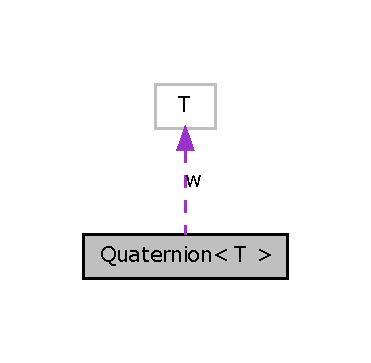
\includegraphics[width=178pt]{class_quaternion__coll__graph}
\end{center}
\end{figure}
\subsection*{Public Member Functions}
\begin{DoxyCompactItemize}
\item 
\hyperlink{class_quaternion_ad5008dba83ccdf61b2e66ac1bfb709f3}{Quaternion} ()
\begin{DoxyCompactList}\small\item\em \hyperlink{class_quaternion}{Quaternion} constructor, sets quaternion to (0 + 0i + 0j + 0k). \item\end{DoxyCompactList}\item 
\hyperlink{class_quaternion_a1737dd209659babb0a71b386dbb63314}{Quaternion} (const \hyperlink{class_quaternion}{Quaternion}$<$ T $>$ \&q)
\begin{DoxyCompactList}\small\item\em Copy constructor. \item\end{DoxyCompactList}\item 
{\footnotesize template$<$class FromT $>$ }\\\hyperlink{class_quaternion_a5e0472cfdc4928db4071c78b1656fe4e}{Quaternion} (const \hyperlink{class_quaternion}{Quaternion}$<$ FromT $>$ \&q)
\begin{DoxyCompactList}\small\item\em Copy casting constructor. \item\end{DoxyCompactList}\item 
\hyperlink{class_quaternion_a6a703f9bd81ff8cb1dac6e5cfebacf5a}{Quaternion} (T w\_\-, const \hyperlink{class_vector3}{Vector3}$<$ T $>$ \&v\_\-)
\begin{DoxyCompactList}\small\item\em Creates quaternion object from real part w\_\- and complex part v\_\-. \item\end{DoxyCompactList}\item 
\hyperlink{class_quaternion_a4d214b9f82b3f74dc7311f584a1eae73}{Quaternion} (T w\_\-, T x, T y, T z)
\begin{DoxyCompactList}\small\item\em Creates quaternion object from value (w\_\- + xi + yj + zk). \item\end{DoxyCompactList}\item 
\hyperlink{class_quaternion}{Quaternion}$<$ T $>$ \& \hyperlink{class_quaternion_ac76403b6bd79b91d21f8d17f3ac938bd}{operator=} (const \hyperlink{class_quaternion}{Quaternion}$<$ T $>$ \&rhs)
\begin{DoxyCompactList}\small\item\em Copy operator. \item\end{DoxyCompactList}\item 
{\footnotesize template$<$class FromT $>$ }\\\hyperlink{class_quaternion}{Quaternion}$<$ T $>$ \& \hyperlink{class_quaternion_ae61051568c9fb1742cb2dc9ad34132c1}{operator=} (const \hyperlink{class_quaternion}{Quaternion}$<$ FromT $>$ \&rhs)
\begin{DoxyCompactList}\small\item\em Copy convert operator. \item\end{DoxyCompactList}\item 
\hyperlink{class_quaternion}{Quaternion}$<$ T $>$ \hyperlink{class_quaternion_a006d553d3e85f86a6426aee06b52e3ac}{operator+} (const \hyperlink{class_quaternion}{Quaternion}$<$ T $>$ \&rhs) const 
\begin{DoxyCompactList}\small\item\em Addition operator. \item\end{DoxyCompactList}\item 
\hyperlink{class_quaternion}{Quaternion}$<$ T $>$ \hyperlink{class_quaternion_ab5b6d22e938709b43398f0bde1a056c8}{operator$\ast$} (const \hyperlink{class_quaternion}{Quaternion}$<$ T $>$ \&rhs) const 
\begin{DoxyCompactList}\small\item\em Multiplication operator. \item\end{DoxyCompactList}\item 
\hyperlink{class_quaternion}{Quaternion}$<$ T $>$ \hyperlink{class_quaternion_ad553f18f44e0466a0f68d60085ba09f7}{operator$\ast$} (T rhs) const 
\begin{DoxyCompactList}\small\item\em Multiplication operator. \item\end{DoxyCompactList}\item 
\hyperlink{class_quaternion}{Quaternion}$<$ T $>$ \hyperlink{class_quaternion_af1dcfe83f758752458d329fa3367b9bd}{operator-\/} (const \hyperlink{class_quaternion}{Quaternion}$<$ T $>$ \&rhs) const 
\begin{DoxyCompactList}\small\item\em Subtraction operator. \item\end{DoxyCompactList}\item 
\hyperlink{class_quaternion}{Quaternion}$<$ T $>$ \& \hyperlink{class_quaternion_a2567e2242703dbb3f82571f47410e553}{operator+=} (const \hyperlink{class_quaternion}{Quaternion}$<$ T $>$ \&rhs)
\begin{DoxyCompactList}\small\item\em Addition operator. \item\end{DoxyCompactList}\item 
\hyperlink{class_quaternion}{Quaternion}$<$ T $>$ \& \hyperlink{class_quaternion_a2d5c3cdfa00f6f978d29dde5de55f067}{operator-\/=} (const \hyperlink{class_quaternion}{Quaternion}$<$ T $>$ \&rhs)
\begin{DoxyCompactList}\small\item\em Subtraction operator. \item\end{DoxyCompactList}\item 
\hyperlink{class_quaternion}{Quaternion}$<$ T $>$ \& \hyperlink{class_quaternion_ac1674c5911091daed8266b997d5a3bdd}{operator$\ast$=} (const \hyperlink{class_quaternion}{Quaternion}$<$ T $>$ \&rhs)
\begin{DoxyCompactList}\small\item\em Multiplication operator. \item\end{DoxyCompactList}\item 
\hyperlink{class_quaternion}{Quaternion}$<$ T $>$ \& \hyperlink{class_quaternion_a25cccfb4a4738744cba0b4b4b47c82ed}{operator$\ast$=} (T rhs)
\begin{DoxyCompactList}\small\item\em Multiplication operator. \item\end{DoxyCompactList}\item 
bool \hyperlink{class_quaternion_ab044ab0bf000fd1ed6937e4861b039e2}{operator==} (const \hyperlink{class_quaternion}{Quaternion}$<$ T $>$ \&rhs) const 
\begin{DoxyCompactList}\small\item\em Equality test operator. \item\end{DoxyCompactList}\item 
bool \hyperlink{class_quaternion_a11892ce300a6e2d830314d795066ee1c}{operator!=} (const \hyperlink{class_quaternion}{Quaternion}$<$ T $>$ \&rhs) const 
\begin{DoxyCompactList}\small\item\em Inequality test operator. \item\end{DoxyCompactList}\item 
\hyperlink{class_quaternion}{Quaternion}$<$ T $>$ \hyperlink{class_quaternion_a2514c9e4a32f140cbac8bb7958d9b855}{operator-\/} () const 
\begin{DoxyCompactList}\small\item\em Unary negate operator. \item\end{DoxyCompactList}\item 
\hyperlink{class_quaternion}{Quaternion}$<$ T $>$ \hyperlink{class_quaternion_ab0393616ac07e35b9808f20bd1740fd5}{operator$\sim$} () const 
\begin{DoxyCompactList}\small\item\em Unary conjugate operator. \item\end{DoxyCompactList}\item 
T \hyperlink{class_quaternion_a47b0bf40eb963350af7c0585c840de0d}{length} () const 
\begin{DoxyCompactList}\small\item\em Get lenght of quaternion. \item\end{DoxyCompactList}\item 
T \hyperlink{class_quaternion_a4e9c538c1c9e2b28ee2399a26efdcbb6}{lengthSq} () const 
\begin{DoxyCompactList}\small\item\em Return square of length. \item\end{DoxyCompactList}\item 
void \hyperlink{class_quaternion_ac27752c31f3bb3620cb757fa3d07cd67}{normalize} ()
\begin{DoxyCompactList}\small\item\em Normalize quaternion. \item\end{DoxyCompactList}\item 
\hyperlink{class_matrix3}{Matrix3}$<$ T $>$ \hyperlink{class_quaternion_a1d74ff2d4fe84758f70b396de5b3f749}{rotMatrix} ()
\begin{DoxyCompactList}\small\item\em Converts quaternion into rotation matrix. \item\end{DoxyCompactList}\item 
\hyperlink{class_matrix4}{Matrix4}$<$ T $>$ \hyperlink{class_quaternion_a00298e05ea5d74c7a25d072b88e20399}{transform} () const 
\begin{DoxyCompactList}\small\item\em Converts quaternion into transformation matrix. \item\end{DoxyCompactList}\item 
\hyperlink{class_quaternion}{Quaternion}$<$ T $>$ \hyperlink{class_quaternion_a8e8e63deaa3c53c63f9dad8556ec1612}{lerp} (T fact, const \hyperlink{class_quaternion}{Quaternion}$<$ T $>$ \&rhs) const 
\begin{DoxyCompactList}\small\item\em Linear interpolation of two quaternions. \item\end{DoxyCompactList}\item 
std::string \hyperlink{class_quaternion_a48b3e7bf721bb2d451dd5845e29f96f2}{toString} () const 
\begin{DoxyCompactList}\small\item\em Gets string representation. \item\end{DoxyCompactList}\item 
\hyperlink{class_quaternion}{Quaternion}$<$ T $>$ \hyperlink{class_quaternion_a6772ea8a4dee0d24913e26c88dc1d3c8}{slerp} (T r, const \hyperlink{class_quaternion}{Quaternion}$<$ T $>$ \&q2) const 
\begin{DoxyCompactList}\small\item\em Computes spherical interpolation between quaternions (this, q2) using coefficient of interpolation r (in \mbox{[}0, 1\mbox{]}). \item\end{DoxyCompactList}\end{DoxyCompactItemize}
\subsection*{Static Public Member Functions}
\begin{DoxyCompactItemize}
\item 
static \hyperlink{class_quaternion}{Quaternion}$<$ T $>$ \hyperlink{class_quaternion_ab7409771454937a4d18e5c65ec237af7}{fromEulerAngles} (T x, T y, T z)
\begin{DoxyCompactList}\small\item\em Creates quaternion for eulers angles. \item\end{DoxyCompactList}\item 
static \hyperlink{class_quaternion}{Quaternion}$<$ T $>$ \hyperlink{class_quaternion_ae1853336ac63f00a63249167ee3b86bd}{fromAxisRot} (\hyperlink{class_vector3}{Vector3}$<$ T $>$ axis, float angleDeg)
\begin{DoxyCompactList}\small\item\em Creates quaternion as rotation around axis. \item\end{DoxyCompactList}\item 
static \hyperlink{class_quaternion}{Quaternion}$<$ T $>$ \hyperlink{class_quaternion_a6444beef0766cd0351408efe45b2a312}{fromMatrix} (const \hyperlink{class_matrix4}{Matrix4}$<$ T $>$ \&m)
\begin{DoxyCompactList}\small\item\em Creates quaternion from transform matrix. \item\end{DoxyCompactList}\item 
static \hyperlink{class_quaternion}{Quaternion}$<$ T $>$ \hyperlink{class_quaternion_a9782ce0b6a21cd183d2c4c6cccbdccb7}{fromMatrix} (const \hyperlink{class_matrix3}{Matrix3}$<$ T $>$ \&m)
\begin{DoxyCompactList}\small\item\em Creates quaternion from rotation matrix. \item\end{DoxyCompactList}\end{DoxyCompactItemize}
\subsection*{Public Attributes}
\begin{DoxyCompactItemize}
\item 
T \hyperlink{class_quaternion_ab3d38cb2d28ba85f00f48768f8fa2815}{w}
\begin{DoxyCompactList}\small\item\em Real part of quaternion. \item\end{DoxyCompactList}\item 
\hyperlink{class_vector3}{Vector3}$<$ T $>$ \hyperlink{class_quaternion_a14b395e80f7c6a1687a824f2adb1eb9b}{v}
\begin{DoxyCompactList}\small\item\em Imaginary part of quaternion. \item\end{DoxyCompactList}\end{DoxyCompactItemize}
\subsection*{Friends}
\begin{DoxyCompactItemize}
\item 
std::ostream \& \hyperlink{class_quaternion_a871c9e237d4b87d722a3e6495f377c23}{operator$<$$<$} (std::ostream \&oss, const \hyperlink{class_quaternion}{Quaternion}$<$ T $>$ \&q)
\begin{DoxyCompactList}\small\item\em Provides output to standard output stream. \item\end{DoxyCompactList}\end{DoxyCompactItemize}


\subsection{Detailed Description}
\subsubsection*{template$<$class T$>$ class Quaternion$<$ T $>$}

\hyperlink{class_quaternion}{Quaternion} class implementing some quaternion algebra operations. \hyperlink{class_quaternion}{Quaternion} is kind of complex number it consists of its real part (w) and its complex part v. This complex part has three elements, so we can express it as xi + yj + zk . Note that coordinates of (x,y,z) are hold inside v field. 

\subsection{Constructor \& Destructor Documentation}
\hypertarget{class_quaternion_ad5008dba83ccdf61b2e66ac1bfb709f3}{
\index{Quaternion@{Quaternion}!Quaternion@{Quaternion}}
\index{Quaternion@{Quaternion}!Quaternion@{Quaternion}}
\subsubsection[{Quaternion}]{\setlength{\rightskip}{0pt plus 5cm}template$<$class T$>$ {\bf Quaternion}$<$ T $>$::{\bf Quaternion} (
\begin{DoxyParamCaption}
{}
\end{DoxyParamCaption}
)\hspace{0.3cm}{\ttfamily  \mbox{[}inline\mbox{]}}}}
\label{class_quaternion_ad5008dba83ccdf61b2e66ac1bfb709f3}


\hyperlink{class_quaternion}{Quaternion} constructor, sets quaternion to (0 + 0i + 0j + 0k). 

\hypertarget{class_quaternion_a1737dd209659babb0a71b386dbb63314}{
\index{Quaternion@{Quaternion}!Quaternion@{Quaternion}}
\index{Quaternion@{Quaternion}!Quaternion@{Quaternion}}
\subsubsection[{Quaternion}]{\setlength{\rightskip}{0pt plus 5cm}template$<$class T$>$ {\bf Quaternion}$<$ T $>$::{\bf Quaternion} (
\begin{DoxyParamCaption}
\item[{const {\bf Quaternion}$<$ T $>$ \&}]{ q}
\end{DoxyParamCaption}
)\hspace{0.3cm}{\ttfamily  \mbox{[}inline\mbox{]}}}}
\label{class_quaternion_a1737dd209659babb0a71b386dbb63314}


Copy constructor. 

\hypertarget{class_quaternion_a5e0472cfdc4928db4071c78b1656fe4e}{
\index{Quaternion@{Quaternion}!Quaternion@{Quaternion}}
\index{Quaternion@{Quaternion}!Quaternion@{Quaternion}}
\subsubsection[{Quaternion}]{\setlength{\rightskip}{0pt plus 5cm}template$<$class T$>$ template$<$class FromT $>$ {\bf Quaternion}$<$ T $>$::{\bf Quaternion} (
\begin{DoxyParamCaption}
\item[{const {\bf Quaternion}$<$ FromT $>$ \&}]{ q}
\end{DoxyParamCaption}
)\hspace{0.3cm}{\ttfamily  \mbox{[}inline\mbox{]}}}}
\label{class_quaternion_a5e0472cfdc4928db4071c78b1656fe4e}


Copy casting constructor. 

\hypertarget{class_quaternion_a6a703f9bd81ff8cb1dac6e5cfebacf5a}{
\index{Quaternion@{Quaternion}!Quaternion@{Quaternion}}
\index{Quaternion@{Quaternion}!Quaternion@{Quaternion}}
\subsubsection[{Quaternion}]{\setlength{\rightskip}{0pt plus 5cm}template$<$class T$>$ {\bf Quaternion}$<$ T $>$::{\bf Quaternion} (
\begin{DoxyParamCaption}
\item[{T}]{ w\_\-, }
\item[{const {\bf Vector3}$<$ T $>$ \&}]{ v\_\-}
\end{DoxyParamCaption}
)\hspace{0.3cm}{\ttfamily  \mbox{[}inline\mbox{]}}}}
\label{class_quaternion_a6a703f9bd81ff8cb1dac6e5cfebacf5a}


Creates quaternion object from real part w\_\- and complex part v\_\-. 


\begin{DoxyParams}{Parameters}
\item[{\em w\_\-}]Real part of quaternion. \item[{\em v\_\-}]Complex part of quaternion (xi + yj + zk). \end{DoxyParams}
\hypertarget{class_quaternion_a4d214b9f82b3f74dc7311f584a1eae73}{
\index{Quaternion@{Quaternion}!Quaternion@{Quaternion}}
\index{Quaternion@{Quaternion}!Quaternion@{Quaternion}}
\subsubsection[{Quaternion}]{\setlength{\rightskip}{0pt plus 5cm}template$<$class T$>$ {\bf Quaternion}$<$ T $>$::{\bf Quaternion} (
\begin{DoxyParamCaption}
\item[{T}]{ w\_\-, }
\item[{T}]{ x, }
\item[{T}]{ y, }
\item[{T}]{ z}
\end{DoxyParamCaption}
)\hspace{0.3cm}{\ttfamily  \mbox{[}inline\mbox{]}}}}
\label{class_quaternion_a4d214b9f82b3f74dc7311f584a1eae73}


Creates quaternion object from value (w\_\- + xi + yj + zk). 


\begin{DoxyParams}{Parameters}
\item[{\em w\_\-}]Real part of quaternion. \item[{\em x}]Complex coefficient for i complex constant. \item[{\em y}]Complex coefficient for j complex constant. \item[{\em z}]Complex coefficient for k complex constant. \end{DoxyParams}


\subsection{Member Function Documentation}
\hypertarget{class_quaternion_ae1853336ac63f00a63249167ee3b86bd}{
\index{Quaternion@{Quaternion}!fromAxisRot@{fromAxisRot}}
\index{fromAxisRot@{fromAxisRot}!Quaternion@{Quaternion}}
\subsubsection[{fromAxisRot}]{\setlength{\rightskip}{0pt plus 5cm}template$<$class T$>$ static {\bf Quaternion}$<$T$>$ {\bf Quaternion}$<$ T $>$::fromAxisRot (
\begin{DoxyParamCaption}
\item[{{\bf Vector3}$<$ T $>$}]{ axis, }
\item[{float}]{ angleDeg}
\end{DoxyParamCaption}
)\hspace{0.3cm}{\ttfamily  \mbox{[}inline, static\mbox{]}}}}
\label{class_quaternion_ae1853336ac63f00a63249167ee3b86bd}


Creates quaternion as rotation around axis. 


\begin{DoxyParams}{Parameters}
\item[{\em axis}]Unit vector expressing axis of rotation. \item[{\em angleDeg}]Angle of rotation around axis (in degrees). \end{DoxyParams}
\hypertarget{class_quaternion_ab7409771454937a4d18e5c65ec237af7}{
\index{Quaternion@{Quaternion}!fromEulerAngles@{fromEulerAngles}}
\index{fromEulerAngles@{fromEulerAngles}!Quaternion@{Quaternion}}
\subsubsection[{fromEulerAngles}]{\setlength{\rightskip}{0pt plus 5cm}template$<$class T$>$ static {\bf Quaternion}$<$T$>$ {\bf Quaternion}$<$ T $>$::fromEulerAngles (
\begin{DoxyParamCaption}
\item[{T}]{ x, }
\item[{T}]{ y, }
\item[{T}]{ z}
\end{DoxyParamCaption}
)\hspace{0.3cm}{\ttfamily  \mbox{[}inline, static\mbox{]}}}}
\label{class_quaternion_ab7409771454937a4d18e5c65ec237af7}


Creates quaternion for eulers angles. 


\begin{DoxyParams}{Parameters}
\item[{\em x}]Rotation around x axis (in degrees). \item[{\em y}]Rotation around y axis (in degrees). \item[{\em z}]Rotation around z axis (in degrees). \end{DoxyParams}
\begin{DoxyReturn}{Returns}
\hyperlink{class_quaternion}{Quaternion} object representing transformation. 
\end{DoxyReturn}
\hypertarget{class_quaternion_a6444beef0766cd0351408efe45b2a312}{
\index{Quaternion@{Quaternion}!fromMatrix@{fromMatrix}}
\index{fromMatrix@{fromMatrix}!Quaternion@{Quaternion}}
\subsubsection[{fromMatrix}]{\setlength{\rightskip}{0pt plus 5cm}template$<$class T$>$ static {\bf Quaternion}$<$T$>$ {\bf Quaternion}$<$ T $>$::fromMatrix (
\begin{DoxyParamCaption}
\item[{const {\bf Matrix4}$<$ T $>$ \&}]{ m}
\end{DoxyParamCaption}
)\hspace{0.3cm}{\ttfamily  \mbox{[}inline, static\mbox{]}}}}
\label{class_quaternion_a6444beef0766cd0351408efe45b2a312}


Creates quaternion from transform matrix. 


\begin{DoxyParams}{Parameters}
\item[{\em m}]Transform matrix used to compute quaternion. \end{DoxyParams}
\begin{DoxyReturn}{Returns}
\hyperlink{class_quaternion}{Quaternion} representing rotation of matrix m. 
\end{DoxyReturn}
\hypertarget{class_quaternion_a9782ce0b6a21cd183d2c4c6cccbdccb7}{
\index{Quaternion@{Quaternion}!fromMatrix@{fromMatrix}}
\index{fromMatrix@{fromMatrix}!Quaternion@{Quaternion}}
\subsubsection[{fromMatrix}]{\setlength{\rightskip}{0pt plus 5cm}template$<$class T$>$ static {\bf Quaternion}$<$T$>$ {\bf Quaternion}$<$ T $>$::fromMatrix (
\begin{DoxyParamCaption}
\item[{const {\bf Matrix3}$<$ T $>$ \&}]{ m}
\end{DoxyParamCaption}
)\hspace{0.3cm}{\ttfamily  \mbox{[}inline, static\mbox{]}}}}
\label{class_quaternion_a9782ce0b6a21cd183d2c4c6cccbdccb7}


Creates quaternion from rotation matrix. 


\begin{DoxyParams}{Parameters}
\item[{\em m}]Rotation matrix used to compute quaternion. \end{DoxyParams}
\begin{DoxyReturn}{Returns}
\hyperlink{class_quaternion}{Quaternion} representing rotation of matrix m. 
\end{DoxyReturn}
\hypertarget{class_quaternion_a47b0bf40eb963350af7c0585c840de0d}{
\index{Quaternion@{Quaternion}!length@{length}}
\index{length@{length}!Quaternion@{Quaternion}}
\subsubsection[{length}]{\setlength{\rightskip}{0pt plus 5cm}template$<$class T$>$ T {\bf Quaternion}$<$ T $>$::length (
\begin{DoxyParamCaption}
{}
\end{DoxyParamCaption}
) const\hspace{0.3cm}{\ttfamily  \mbox{[}inline\mbox{]}}}}
\label{class_quaternion_a47b0bf40eb963350af7c0585c840de0d}


Get lenght of quaternion. 

\begin{DoxyReturn}{Returns}
Length of quaternion. 
\end{DoxyReturn}
\hypertarget{class_quaternion_a4e9c538c1c9e2b28ee2399a26efdcbb6}{
\index{Quaternion@{Quaternion}!lengthSq@{lengthSq}}
\index{lengthSq@{lengthSq}!Quaternion@{Quaternion}}
\subsubsection[{lengthSq}]{\setlength{\rightskip}{0pt plus 5cm}template$<$class T$>$ T {\bf Quaternion}$<$ T $>$::lengthSq (
\begin{DoxyParamCaption}
{}
\end{DoxyParamCaption}
) const\hspace{0.3cm}{\ttfamily  \mbox{[}inline\mbox{]}}}}
\label{class_quaternion_a4e9c538c1c9e2b28ee2399a26efdcbb6}


Return square of length. 

\begin{DoxyReturn}{Returns}
length $^\wedge$ 2 
\end{DoxyReturn}
\begin{DoxyNote}{Note}
This method is faster then \hyperlink{class_quaternion_a47b0bf40eb963350af7c0585c840de0d}{length()}. For comparison of length of two quaternion can be used just this value, instead of more expensive \hyperlink{class_quaternion_a47b0bf40eb963350af7c0585c840de0d}{length()} method. 
\end{DoxyNote}
\hypertarget{class_quaternion_a8e8e63deaa3c53c63f9dad8556ec1612}{
\index{Quaternion@{Quaternion}!lerp@{lerp}}
\index{lerp@{lerp}!Quaternion@{Quaternion}}
\subsubsection[{lerp}]{\setlength{\rightskip}{0pt plus 5cm}template$<$class T$>$ {\bf Quaternion}$<$T$>$ {\bf Quaternion}$<$ T $>$::lerp (
\begin{DoxyParamCaption}
\item[{T}]{ fact, }
\item[{const {\bf Quaternion}$<$ T $>$ \&}]{ rhs}
\end{DoxyParamCaption}
) const\hspace{0.3cm}{\ttfamily  \mbox{[}inline\mbox{]}}}}
\label{class_quaternion_a8e8e63deaa3c53c63f9dad8556ec1612}


Linear interpolation of two quaternions. 


\begin{DoxyParams}{Parameters}
\item[{\em fact}]Factor of interpolation. For translation from position of this vector to quaternion rhs, values of factor goes from 0.0 to 1.0. \item[{\em rhs}]Second \hyperlink{class_quaternion}{Quaternion} for interpolation \end{DoxyParams}
\begin{DoxyNote}{Note}
However values of fact parameter are reasonable only in interval \mbox{[}0.0 , 1.0\mbox{]}, you can pass also values outside of this interval and you can get result (extrapolation?) 
\end{DoxyNote}
\hypertarget{class_quaternion_ac27752c31f3bb3620cb757fa3d07cd67}{
\index{Quaternion@{Quaternion}!normalize@{normalize}}
\index{normalize@{normalize}!Quaternion@{Quaternion}}
\subsubsection[{normalize}]{\setlength{\rightskip}{0pt plus 5cm}template$<$class T$>$ void {\bf Quaternion}$<$ T $>$::normalize (
\begin{DoxyParamCaption}
{}
\end{DoxyParamCaption}
)\hspace{0.3cm}{\ttfamily  \mbox{[}inline\mbox{]}}}}
\label{class_quaternion_ac27752c31f3bb3620cb757fa3d07cd67}


Normalize quaternion. 

\hypertarget{class_quaternion_a11892ce300a6e2d830314d795066ee1c}{
\index{Quaternion@{Quaternion}!operator!=@{operator!=}}
\index{operator!=@{operator!=}!Quaternion@{Quaternion}}
\subsubsection[{operator!=}]{\setlength{\rightskip}{0pt plus 5cm}template$<$class T$>$ bool {\bf Quaternion}$<$ T $>$::operator!= (
\begin{DoxyParamCaption}
\item[{const {\bf Quaternion}$<$ T $>$ \&}]{ rhs}
\end{DoxyParamCaption}
) const\hspace{0.3cm}{\ttfamily  \mbox{[}inline\mbox{]}}}}
\label{class_quaternion_a11892ce300a6e2d830314d795066ee1c}


Inequality test operator. 


\begin{DoxyParams}{Parameters}
\item[{\em rhs}]Right hand side argument of binary operator. \end{DoxyParams}
\begin{DoxyReturn}{Returns}
not (lhs == rhs) :-\/P 
\end{DoxyReturn}
\hypertarget{class_quaternion_ad553f18f44e0466a0f68d60085ba09f7}{
\index{Quaternion@{Quaternion}!operator$\ast$@{operator$\ast$}}
\index{operator$\ast$@{operator$\ast$}!Quaternion@{Quaternion}}
\subsubsection[{operator$\ast$}]{\setlength{\rightskip}{0pt plus 5cm}template$<$class T$>$ {\bf Quaternion}$<$T$>$ {\bf Quaternion}$<$ T $>$::operator$\ast$ (
\begin{DoxyParamCaption}
\item[{T}]{ rhs}
\end{DoxyParamCaption}
) const\hspace{0.3cm}{\ttfamily  \mbox{[}inline\mbox{]}}}}
\label{class_quaternion_ad553f18f44e0466a0f68d60085ba09f7}


Multiplication operator. 


\begin{DoxyParams}{Parameters}
\item[{\em rhs}]Right hand side argument of binary operator. \end{DoxyParams}
\hypertarget{class_quaternion_ab5b6d22e938709b43398f0bde1a056c8}{
\index{Quaternion@{Quaternion}!operator$\ast$@{operator$\ast$}}
\index{operator$\ast$@{operator$\ast$}!Quaternion@{Quaternion}}
\subsubsection[{operator$\ast$}]{\setlength{\rightskip}{0pt plus 5cm}template$<$class T$>$ {\bf Quaternion}$<$T$>$ {\bf Quaternion}$<$ T $>$::operator$\ast$ (
\begin{DoxyParamCaption}
\item[{const {\bf Quaternion}$<$ T $>$ \&}]{ rhs}
\end{DoxyParamCaption}
) const\hspace{0.3cm}{\ttfamily  \mbox{[}inline\mbox{]}}}}
\label{class_quaternion_ab5b6d22e938709b43398f0bde1a056c8}


Multiplication operator. 


\begin{DoxyParams}{Parameters}
\item[{\em rhs}]Right hand side argument of binary operator. \end{DoxyParams}
\hypertarget{class_quaternion_ac1674c5911091daed8266b997d5a3bdd}{
\index{Quaternion@{Quaternion}!operator$\ast$=@{operator$\ast$=}}
\index{operator$\ast$=@{operator$\ast$=}!Quaternion@{Quaternion}}
\subsubsection[{operator$\ast$=}]{\setlength{\rightskip}{0pt plus 5cm}template$<$class T$>$ {\bf Quaternion}$<$T$>$\& {\bf Quaternion}$<$ T $>$::operator$\ast$= (
\begin{DoxyParamCaption}
\item[{const {\bf Quaternion}$<$ T $>$ \&}]{ rhs}
\end{DoxyParamCaption}
)\hspace{0.3cm}{\ttfamily  \mbox{[}inline\mbox{]}}}}
\label{class_quaternion_ac1674c5911091daed8266b997d5a3bdd}


Multiplication operator. 


\begin{DoxyParams}{Parameters}
\item[{\em rhs}]Right hand side argument of binary operator. \end{DoxyParams}
\hypertarget{class_quaternion_a25cccfb4a4738744cba0b4b4b47c82ed}{
\index{Quaternion@{Quaternion}!operator$\ast$=@{operator$\ast$=}}
\index{operator$\ast$=@{operator$\ast$=}!Quaternion@{Quaternion}}
\subsubsection[{operator$\ast$=}]{\setlength{\rightskip}{0pt plus 5cm}template$<$class T$>$ {\bf Quaternion}$<$T$>$\& {\bf Quaternion}$<$ T $>$::operator$\ast$= (
\begin{DoxyParamCaption}
\item[{T}]{ rhs}
\end{DoxyParamCaption}
)\hspace{0.3cm}{\ttfamily  \mbox{[}inline\mbox{]}}}}
\label{class_quaternion_a25cccfb4a4738744cba0b4b4b47c82ed}


Multiplication operator. 


\begin{DoxyParams}{Parameters}
\item[{\em rhs}]Right hand side argument of binary operator. \end{DoxyParams}
\hypertarget{class_quaternion_a006d553d3e85f86a6426aee06b52e3ac}{
\index{Quaternion@{Quaternion}!operator+@{operator+}}
\index{operator+@{operator+}!Quaternion@{Quaternion}}
\subsubsection[{operator+}]{\setlength{\rightskip}{0pt plus 5cm}template$<$class T$>$ {\bf Quaternion}$<$T$>$ {\bf Quaternion}$<$ T $>$::operator+ (
\begin{DoxyParamCaption}
\item[{const {\bf Quaternion}$<$ T $>$ \&}]{ rhs}
\end{DoxyParamCaption}
) const\hspace{0.3cm}{\ttfamily  \mbox{[}inline\mbox{]}}}}
\label{class_quaternion_a006d553d3e85f86a6426aee06b52e3ac}


Addition operator. 


\begin{DoxyParams}{Parameters}
\item[{\em rhs}]Right hand side argument of binary operator. \end{DoxyParams}
\hypertarget{class_quaternion_a2567e2242703dbb3f82571f47410e553}{
\index{Quaternion@{Quaternion}!operator+=@{operator+=}}
\index{operator+=@{operator+=}!Quaternion@{Quaternion}}
\subsubsection[{operator+=}]{\setlength{\rightskip}{0pt plus 5cm}template$<$class T$>$ {\bf Quaternion}$<$T$>$\& {\bf Quaternion}$<$ T $>$::operator+= (
\begin{DoxyParamCaption}
\item[{const {\bf Quaternion}$<$ T $>$ \&}]{ rhs}
\end{DoxyParamCaption}
)\hspace{0.3cm}{\ttfamily  \mbox{[}inline\mbox{]}}}}
\label{class_quaternion_a2567e2242703dbb3f82571f47410e553}


Addition operator. 


\begin{DoxyParams}{Parameters}
\item[{\em rhs}]Right hand side argument of binary operator. \end{DoxyParams}
\hypertarget{class_quaternion_a2514c9e4a32f140cbac8bb7958d9b855}{
\index{Quaternion@{Quaternion}!operator-\/@{operator-\/}}
\index{operator-\/@{operator-\/}!Quaternion@{Quaternion}}
\subsubsection[{operator-\/}]{\setlength{\rightskip}{0pt plus 5cm}template$<$class T$>$ {\bf Quaternion}$<$T$>$ {\bf Quaternion}$<$ T $>$::operator-\/ (
\begin{DoxyParamCaption}
{}
\end{DoxyParamCaption}
) const\hspace{0.3cm}{\ttfamily  \mbox{[}inline\mbox{]}}}}
\label{class_quaternion_a2514c9e4a32f140cbac8bb7958d9b855}


Unary negate operator. 

\begin{DoxyReturn}{Returns}
negated quaternion 
\end{DoxyReturn}
\hypertarget{class_quaternion_af1dcfe83f758752458d329fa3367b9bd}{
\index{Quaternion@{Quaternion}!operator-\/@{operator-\/}}
\index{operator-\/@{operator-\/}!Quaternion@{Quaternion}}
\subsubsection[{operator-\/}]{\setlength{\rightskip}{0pt plus 5cm}template$<$class T$>$ {\bf Quaternion}$<$T$>$ {\bf Quaternion}$<$ T $>$::operator-\/ (
\begin{DoxyParamCaption}
\item[{const {\bf Quaternion}$<$ T $>$ \&}]{ rhs}
\end{DoxyParamCaption}
) const\hspace{0.3cm}{\ttfamily  \mbox{[}inline\mbox{]}}}}
\label{class_quaternion_af1dcfe83f758752458d329fa3367b9bd}


Subtraction operator. 


\begin{DoxyParams}{Parameters}
\item[{\em rhs}]Right hand side argument of binary operator. \end{DoxyParams}
\hypertarget{class_quaternion_a2d5c3cdfa00f6f978d29dde5de55f067}{
\index{Quaternion@{Quaternion}!operator-\/=@{operator-\/=}}
\index{operator-\/=@{operator-\/=}!Quaternion@{Quaternion}}
\subsubsection[{operator-\/=}]{\setlength{\rightskip}{0pt plus 5cm}template$<$class T$>$ {\bf Quaternion}$<$T$>$\& {\bf Quaternion}$<$ T $>$::operator-\/= (
\begin{DoxyParamCaption}
\item[{const {\bf Quaternion}$<$ T $>$ \&}]{ rhs}
\end{DoxyParamCaption}
)\hspace{0.3cm}{\ttfamily  \mbox{[}inline\mbox{]}}}}
\label{class_quaternion_a2d5c3cdfa00f6f978d29dde5de55f067}


Subtraction operator. 


\begin{DoxyParams}{Parameters}
\item[{\em rhs}]Right hand side argument of binary operator. \end{DoxyParams}
\hypertarget{class_quaternion_ae61051568c9fb1742cb2dc9ad34132c1}{
\index{Quaternion@{Quaternion}!operator=@{operator=}}
\index{operator=@{operator=}!Quaternion@{Quaternion}}
\subsubsection[{operator=}]{\setlength{\rightskip}{0pt plus 5cm}template$<$class T$>$ template$<$class FromT $>$ {\bf Quaternion}$<$T$>$\& {\bf Quaternion}$<$ T $>$::operator= (
\begin{DoxyParamCaption}
\item[{const {\bf Quaternion}$<$ FromT $>$ \&}]{ rhs}
\end{DoxyParamCaption}
)\hspace{0.3cm}{\ttfamily  \mbox{[}inline\mbox{]}}}}
\label{class_quaternion_ae61051568c9fb1742cb2dc9ad34132c1}


Copy convert operator. 


\begin{DoxyParams}{Parameters}
\item[{\em rhs}]Right hand side argument of binary operator. \end{DoxyParams}
\hypertarget{class_quaternion_ac76403b6bd79b91d21f8d17f3ac938bd}{
\index{Quaternion@{Quaternion}!operator=@{operator=}}
\index{operator=@{operator=}!Quaternion@{Quaternion}}
\subsubsection[{operator=}]{\setlength{\rightskip}{0pt plus 5cm}template$<$class T$>$ {\bf Quaternion}$<$T$>$\& {\bf Quaternion}$<$ T $>$::operator= (
\begin{DoxyParamCaption}
\item[{const {\bf Quaternion}$<$ T $>$ \&}]{ rhs}
\end{DoxyParamCaption}
)\hspace{0.3cm}{\ttfamily  \mbox{[}inline\mbox{]}}}}
\label{class_quaternion_ac76403b6bd79b91d21f8d17f3ac938bd}


Copy operator. 


\begin{DoxyParams}{Parameters}
\item[{\em rhs}]Right hand side argument of binary operator. \end{DoxyParams}
\hypertarget{class_quaternion_ab044ab0bf000fd1ed6937e4861b039e2}{
\index{Quaternion@{Quaternion}!operator==@{operator==}}
\index{operator==@{operator==}!Quaternion@{Quaternion}}
\subsubsection[{operator==}]{\setlength{\rightskip}{0pt plus 5cm}template$<$class T$>$ bool {\bf Quaternion}$<$ T $>$::operator== (
\begin{DoxyParamCaption}
\item[{const {\bf Quaternion}$<$ T $>$ \&}]{ rhs}
\end{DoxyParamCaption}
) const\hspace{0.3cm}{\ttfamily  \mbox{[}inline\mbox{]}}}}
\label{class_quaternion_ab044ab0bf000fd1ed6937e4861b039e2}


Equality test operator. 


\begin{DoxyParams}{Parameters}
\item[{\em rhs}]Right hand side argument of binary operator. \end{DoxyParams}
\begin{DoxyNote}{Note}
Test of equality is based of threshold EPSILON value. To be two values equal, must satisfy this condition $|$ lhs -\/ rhs $|$ $<$ EPSILON, for all quaternion coordinates. 
\end{DoxyNote}
\hypertarget{class_quaternion_ab0393616ac07e35b9808f20bd1740fd5}{
\index{Quaternion@{Quaternion}!operator$\sim$@{operator$\sim$}}
\index{operator$\sim$@{operator$\sim$}!Quaternion@{Quaternion}}
\subsubsection[{operator$\sim$}]{\setlength{\rightskip}{0pt plus 5cm}template$<$class T$>$ {\bf Quaternion}$<$T$>$ {\bf Quaternion}$<$ T $>$::operator$\sim$ (
\begin{DoxyParamCaption}
{}
\end{DoxyParamCaption}
) const\hspace{0.3cm}{\ttfamily  \mbox{[}inline\mbox{]}}}}
\label{class_quaternion_ab0393616ac07e35b9808f20bd1740fd5}


Unary conjugate operator. 

\begin{DoxyReturn}{Returns}
conjugated quaternion 
\end{DoxyReturn}
\hypertarget{class_quaternion_a1d74ff2d4fe84758f70b396de5b3f749}{
\index{Quaternion@{Quaternion}!rotMatrix@{rotMatrix}}
\index{rotMatrix@{rotMatrix}!Quaternion@{Quaternion}}
\subsubsection[{rotMatrix}]{\setlength{\rightskip}{0pt plus 5cm}template$<$class T$>$ {\bf Matrix3}$<$T$>$ {\bf Quaternion}$<$ T $>$::rotMatrix (
\begin{DoxyParamCaption}
{}
\end{DoxyParamCaption}
)\hspace{0.3cm}{\ttfamily  \mbox{[}inline\mbox{]}}}}
\label{class_quaternion_a1d74ff2d4fe84758f70b396de5b3f749}


Converts quaternion into rotation matrix. 

\begin{DoxyReturn}{Returns}
Rotation matrix expressing this quaternion. 
\end{DoxyReturn}
\hypertarget{class_quaternion_a6772ea8a4dee0d24913e26c88dc1d3c8}{
\index{Quaternion@{Quaternion}!slerp@{slerp}}
\index{slerp@{slerp}!Quaternion@{Quaternion}}
\subsubsection[{slerp}]{\setlength{\rightskip}{0pt plus 5cm}template$<$class T$>$ {\bf Quaternion}$<$T$>$ {\bf Quaternion}$<$ T $>$::slerp (
\begin{DoxyParamCaption}
\item[{T}]{ r, }
\item[{const {\bf Quaternion}$<$ T $>$ \&}]{ q2}
\end{DoxyParamCaption}
) const\hspace{0.3cm}{\ttfamily  \mbox{[}inline\mbox{]}}}}
\label{class_quaternion_a6772ea8a4dee0d24913e26c88dc1d3c8}


Computes spherical interpolation between quaternions (this, q2) using coefficient of interpolation r (in \mbox{[}0, 1\mbox{]}). 


\begin{DoxyParams}{Parameters}
\item[{\em r}]The ratio of interpolation form this (r = 0) to q2 (r = 1). \item[{\em q2}]Second quaternion for interpolation. \end{DoxyParams}
\begin{DoxyReturn}{Returns}
Result of interpolation. 
\end{DoxyReturn}
\hypertarget{class_quaternion_a48b3e7bf721bb2d451dd5845e29f96f2}{
\index{Quaternion@{Quaternion}!toString@{toString}}
\index{toString@{toString}!Quaternion@{Quaternion}}
\subsubsection[{toString}]{\setlength{\rightskip}{0pt plus 5cm}template$<$class T$>$ std::string {\bf Quaternion}$<$ T $>$::toString (
\begin{DoxyParamCaption}
{}
\end{DoxyParamCaption}
) const\hspace{0.3cm}{\ttfamily  \mbox{[}inline\mbox{]}}}}
\label{class_quaternion_a48b3e7bf721bb2d451dd5845e29f96f2}


Gets string representation. 

\hypertarget{class_quaternion_a00298e05ea5d74c7a25d072b88e20399}{
\index{Quaternion@{Quaternion}!transform@{transform}}
\index{transform@{transform}!Quaternion@{Quaternion}}
\subsubsection[{transform}]{\setlength{\rightskip}{0pt plus 5cm}template$<$class T$>$ {\bf Matrix4}$<$T$>$ {\bf Quaternion}$<$ T $>$::transform (
\begin{DoxyParamCaption}
{}
\end{DoxyParamCaption}
) const\hspace{0.3cm}{\ttfamily  \mbox{[}inline\mbox{]}}}}
\label{class_quaternion_a00298e05ea5d74c7a25d072b88e20399}


Converts quaternion into transformation matrix. 

\begin{DoxyNote}{Note}
This method performs same operation as \hyperlink{class_quaternion_a1d74ff2d4fe84758f70b396de5b3f749}{rotMatrix()} conversion method. But returns Matrix of 4x4 elements. 
\end{DoxyNote}
\begin{DoxyReturn}{Returns}
Transformation matrix expressing this quaternion. 
\end{DoxyReturn}


\subsection{Friends And Related Function Documentation}
\hypertarget{class_quaternion_a871c9e237d4b87d722a3e6495f377c23}{
\index{Quaternion@{Quaternion}!operator$<$$<$@{operator$<$$<$}}
\index{operator$<$$<$@{operator$<$$<$}!Quaternion@{Quaternion}}
\subsubsection[{operator$<$$<$}]{\setlength{\rightskip}{0pt plus 5cm}template$<$class T$>$ std::ostream\& operator$<$$<$ (
\begin{DoxyParamCaption}
\item[{std::ostream \&}]{ oss, }
\item[{const {\bf Quaternion}$<$ T $>$ \&}]{ q}
\end{DoxyParamCaption}
)\hspace{0.3cm}{\ttfamily  \mbox{[}friend\mbox{]}}}}
\label{class_quaternion_a871c9e237d4b87d722a3e6495f377c23}


Provides output to standard output stream. 



\subsection{Member Data Documentation}
\hypertarget{class_quaternion_a14b395e80f7c6a1687a824f2adb1eb9b}{
\index{Quaternion@{Quaternion}!v@{v}}
\index{v@{v}!Quaternion@{Quaternion}}
\subsubsection[{v}]{\setlength{\rightskip}{0pt plus 5cm}template$<$class T$>$ {\bf Vector3}$<$T$>$ {\bf Quaternion}$<$ T $>$::{\bf v}}}
\label{class_quaternion_a14b395e80f7c6a1687a824f2adb1eb9b}


Imaginary part of quaternion. 

\hypertarget{class_quaternion_ab3d38cb2d28ba85f00f48768f8fa2815}{
\index{Quaternion@{Quaternion}!w@{w}}
\index{w@{w}!Quaternion@{Quaternion}}
\subsubsection[{w}]{\setlength{\rightskip}{0pt plus 5cm}template$<$class T$>$ T {\bf Quaternion}$<$ T $>$::{\bf w}}}
\label{class_quaternion_ab3d38cb2d28ba85f00f48768f8fa2815}


Real part of quaternion. 



The documentation for this class was generated from the following file:\begin{DoxyCompactItemize}
\item 
src/\hyperlink{vmath_8h}{vmath.h}\end{DoxyCompactItemize}

\hypertarget{class_vector2}{
\section{Vector2$<$ T $>$ Class Template Reference}
\label{class_vector2}\index{Vector2@{Vector2}}
}


Class for two dimensional vector.  




{\ttfamily \#include $<$vmath.h$>$}



Collaboration diagram for Vector2$<$ T $>$:
\nopagebreak
\begin{figure}[H]
\begin{center}
\leavevmode
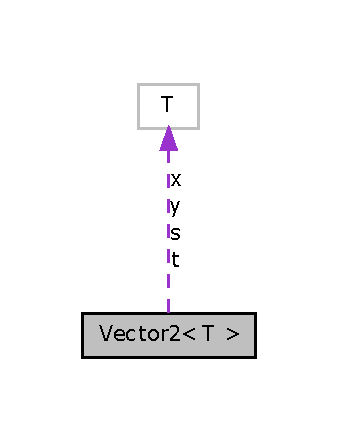
\includegraphics[width=162pt]{class_vector2__coll__graph}
\end{center}
\end{figure}
\subsection*{Public Member Functions}
\begin{DoxyCompactItemize}
\item 
\hyperlink{class_vector2_ae2f1223cb0d664aa73afb789086a4174}{Vector2} ()
\begin{DoxyCompactList}\small\item\em Creates and sets to (0,0). \item\end{DoxyCompactList}\item 
\hyperlink{class_vector2_a73dbb934192bdaffb43f4f472e62d1d7}{Vector2} (T nx, T ny)
\begin{DoxyCompactList}\small\item\em Creates and sets to (x,y). \item\end{DoxyCompactList}\item 
\hyperlink{class_vector2_a6942368710d42c4b66776538a583d6dc}{Vector2} (const \hyperlink{class_vector2}{Vector2}$<$ T $>$ \&src)
\begin{DoxyCompactList}\small\item\em Copy constructor. \item\end{DoxyCompactList}\item 
{\footnotesize template$<$class FromT $>$ }\\\hyperlink{class_vector2_a93286dc1ccd8e1f2deb49668076aa5dc}{Vector2} (const \hyperlink{class_vector2}{Vector2}$<$ FromT $>$ \&src)
\begin{DoxyCompactList}\small\item\em Copy casting constructor. \item\end{DoxyCompactList}\item 
{\footnotesize template$<$class FromT $>$ }\\\hyperlink{class_vector2}{Vector2}$<$ T $>$ \& \hyperlink{class_vector2_aa93d791f8624cf19ea3b2a7eed329b61}{operator=} (const \hyperlink{class_vector2}{Vector2}$<$ FromT $>$ \&rhs)
\begin{DoxyCompactList}\small\item\em Copy casting operator. \item\end{DoxyCompactList}\item 
\hyperlink{class_vector2}{Vector2}$<$ T $>$ \& \hyperlink{class_vector2_a63e1c003cecacae0b26296941b3fe44a}{operator=} (const \hyperlink{class_vector2}{Vector2}$<$ T $>$ \&rhs)
\begin{DoxyCompactList}\small\item\em Copy operator. \item\end{DoxyCompactList}\item 
T \& \hyperlink{class_vector2_a7d7e7b0abc5433808832147bfd58c171}{operator\mbox{[}$\,$\mbox{]}} (int n)
\begin{DoxyCompactList}\small\item\em Array access operator. \item\end{DoxyCompactList}\item 
const T \& \hyperlink{class_vector2_a33a7b603ccfa18de8524effcb18388df}{operator\mbox{[}$\,$\mbox{]}} (int n) const 
\begin{DoxyCompactList}\small\item\em Constant array access operator. \item\end{DoxyCompactList}\item 
\hyperlink{class_vector2}{Vector2}$<$ T $>$ \hyperlink{class_vector2_a481bea0de6a8060118b48a4f2516e329}{operator+} (const \hyperlink{class_vector2}{Vector2}$<$ T $>$ \&rhs) const 
\begin{DoxyCompactList}\small\item\em Addition operator. \item\end{DoxyCompactList}\item 
\hyperlink{class_vector2}{Vector2}$<$ T $>$ \hyperlink{class_vector2_acb95b5aa975ef2eccaafc9314ed31373}{operator-\/} (const \hyperlink{class_vector2}{Vector2}$<$ T $>$ \&rhs) const 
\begin{DoxyCompactList}\small\item\em Subtraction operator. \item\end{DoxyCompactList}\item 
\hyperlink{class_vector2}{Vector2}$<$ T $>$ \hyperlink{class_vector2_a400c2c32b1b54f5423ddcb6e24d90c6a}{operator$\ast$} (const \hyperlink{class_vector2}{Vector2}$<$ T $>$ \&rhs) const 
\begin{DoxyCompactList}\small\item\em Multiplication operator. \item\end{DoxyCompactList}\item 
\hyperlink{class_vector2}{Vector2}$<$ T $>$ \hyperlink{class_vector2_a7ca23b6847d15c9e0b8544071c08a0c9}{operator/} (const \hyperlink{class_vector2}{Vector2}$<$ T $>$ \&rhs) const 
\begin{DoxyCompactList}\small\item\em Division operator. \item\end{DoxyCompactList}\item 
\hyperlink{class_vector2}{Vector2}$<$ T $>$ \& \hyperlink{class_vector2_ac81fd06dc944404ab96e387a9c810d41}{operator+=} (const \hyperlink{class_vector2}{Vector2}$<$ T $>$ \&rhs)
\begin{DoxyCompactList}\small\item\em Addition operator. \item\end{DoxyCompactList}\item 
\hyperlink{class_vector2}{Vector2}$<$ T $>$ \& \hyperlink{class_vector2_adf7f03dd1b698850baaff61b21ec501f}{operator-\/=} (const \hyperlink{class_vector2}{Vector2}$<$ T $>$ \&rhs)
\begin{DoxyCompactList}\small\item\em Substraction operator. \item\end{DoxyCompactList}\item 
\hyperlink{class_vector2}{Vector2}$<$ T $>$ \& \hyperlink{class_vector2_aefae77616723d6c857a3e21dd5ea70e7}{operator$\ast$=} (const \hyperlink{class_vector2}{Vector2}$<$ T $>$ \&rhs)
\begin{DoxyCompactList}\small\item\em Multiplication operator. \item\end{DoxyCompactList}\item 
\hyperlink{class_vector2}{Vector2}$<$ T $>$ \& \hyperlink{class_vector2_a7cf62fe9339f503b680daaeacc71eb4c}{operator/=} (const \hyperlink{class_vector2}{Vector2}$<$ T $>$ \&rhs)
\begin{DoxyCompactList}\small\item\em Division operator. \item\end{DoxyCompactList}\item 
\hyperlink{class_vector2}{Vector2}$<$ T $>$ \hyperlink{class_vector2_a17527e8fe674085b892ccfcb42cd85b3}{operator+} (T rhs) const 
\begin{DoxyCompactList}\small\item\em Addition operator. \item\end{DoxyCompactList}\item 
\hyperlink{class_vector2}{Vector2}$<$ T $>$ \hyperlink{class_vector2_ac6729c8cb9d0eb0a5f1aeb3093c1669f}{operator-\/} (T rhs) const 
\begin{DoxyCompactList}\small\item\em Subtraction operator. \item\end{DoxyCompactList}\item 
\hyperlink{class_vector2}{Vector2}$<$ T $>$ \hyperlink{class_vector2_afe8640177b4a4114196b5d4f6a2ee597}{operator$\ast$} (T rhs) const 
\begin{DoxyCompactList}\small\item\em Multiplication operator. \item\end{DoxyCompactList}\item 
\hyperlink{class_vector2}{Vector2}$<$ T $>$ \hyperlink{class_vector2_a4c504fd30766b8d3f50a1871590147a8}{operator/} (T rhs) const 
\begin{DoxyCompactList}\small\item\em Division operator. \item\end{DoxyCompactList}\item 
\hyperlink{class_vector2}{Vector2}$<$ T $>$ \& \hyperlink{class_vector2_ac9fc3a535e3e2c4a001db064b0572a89}{operator+=} (T rhs)
\begin{DoxyCompactList}\small\item\em Addition operator. \item\end{DoxyCompactList}\item 
\hyperlink{class_vector2}{Vector2}$<$ T $>$ \& \hyperlink{class_vector2_afba0b8c23b74f538ab8cecf8c77d9a17}{operator-\/=} (T rhs)
\begin{DoxyCompactList}\small\item\em Subtraction operator. \item\end{DoxyCompactList}\item 
\hyperlink{class_vector2}{Vector2}$<$ T $>$ \& \hyperlink{class_vector2_ad71db03f38ea0f7b0794bf7c12d04c39}{operator$\ast$=} (T rhs)
\begin{DoxyCompactList}\small\item\em Multiplication operator. \item\end{DoxyCompactList}\item 
\hyperlink{class_vector2}{Vector2}$<$ T $>$ \& \hyperlink{class_vector2_ab50c18ba014384a42cc78be9a36a222c}{operator/=} (T rhs)
\begin{DoxyCompactList}\small\item\em Division operator. \item\end{DoxyCompactList}\item 
bool \hyperlink{class_vector2_af44452c8cd74b57249f334fe3a0e5212}{operator==} (const \hyperlink{class_vector2}{Vector2}$<$ T $>$ \&rhs) const 
\begin{DoxyCompactList}\small\item\em Equality test operator. \item\end{DoxyCompactList}\item 
bool \hyperlink{class_vector2_a0c69e0a4ef5fdfdd5800525c7a751f08}{operator!=} (const \hyperlink{class_vector2}{Vector2}$<$ T $>$ \&rhs) const 
\begin{DoxyCompactList}\small\item\em Inequality test operator. \item\end{DoxyCompactList}\item 
\hyperlink{class_vector2}{Vector2}$<$ T $>$ \hyperlink{class_vector2_aa1367fe9fa837cd5dab8c9b57de5db6a}{operator-\/} () const 
\begin{DoxyCompactList}\small\item\em Unary negate operator. \item\end{DoxyCompactList}\item 
T \hyperlink{class_vector2_a119c51f16f90ffb3b30ee59475e7fdf8}{length} () const 
\begin{DoxyCompactList}\small\item\em Get length of vector. \item\end{DoxyCompactList}\item 
void \hyperlink{class_vector2_ace2a626eaa79412e2946216e9c3e63c6}{normalize} ()
\begin{DoxyCompactList}\small\item\em Normalize vector. \item\end{DoxyCompactList}\item 
T \hyperlink{class_vector2_a54aeb0e64f05cb4eb6787b6ac9f9a468}{lengthSq} () const 
\begin{DoxyCompactList}\small\item\em Return square of length. \item\end{DoxyCompactList}\item 
\hyperlink{class_vector2}{Vector2}$<$ T $>$ \hyperlink{class_vector2_a1377e154f9f49724dbf28e2d6f43fe66}{lerp} (T fact, const \hyperlink{class_vector2}{Vector2}$<$ T $>$ \&r) const 
\begin{DoxyCompactList}\small\item\em Linear interpolation of two vectors. \item\end{DoxyCompactList}\item 
\hyperlink{class_vector2_a47ef81d7cef209446129a056b0d20099}{operator T $\ast$} ()
\begin{DoxyCompactList}\small\item\em Conversion to pointer operator. \item\end{DoxyCompactList}\item 
\hyperlink{class_vector2_a8da0db93360db67497ee7614e1152a4f}{operator const T $\ast$} () const 
\begin{DoxyCompactList}\small\item\em Conversion to pointer operator. \item\end{DoxyCompactList}\item 
std::string \hyperlink{class_vector2_a4c82882017e78c4d36aa1584b8c4aa69}{toString} () const 
\begin{DoxyCompactList}\small\item\em Gets string representation. \item\end{DoxyCompactList}\end{DoxyCompactItemize}
\subsection*{Public Attributes}
\begin{DoxyCompactItemize}
\item 
\begin{tabbing}
xx\=xx\=xx\=xx\=xx\=xx\=xx\=xx\=xx\=\kill
union \{\\
\>T \hyperlink{class_vector2_a78fa1f2ed5e261c7fbeb8f3536a1ee34}{x}\\
\>\>{\em First element of vector, alias for X-\/coordinate. }\\
\>T \hyperlink{class_vector2_a4855e78bb8bc73048d7871e414047ecc}{s}\\
\>\>{\em First element of vector, alias for S-\/coordinate. }\\
\}; \\

\end{tabbing}\item 
\begin{tabbing}
xx\=xx\=xx\=xx\=xx\=xx\=xx\=xx\=xx\=\kill
union \{\\
\>T \hyperlink{class_vector2_a6cfed8355591aa269f4dba43bd806ef9}{y}\\
\>\>{\em Second element of vector, alias for Y-\/coordinate. }\\
\>T \hyperlink{class_vector2_afdb6c2a84434bb86bd5e8a92a546c91a}{t}\\
\>\>{\em Second element of vector, alias for T-\/coordinate. }\\
\}; \\

\end{tabbing}\end{DoxyCompactItemize}
\subsection*{Friends}
\begin{DoxyCompactItemize}
\item 
std::ostream \& \hyperlink{class_vector2_a1d59d3600fcf2d9886c3664ae6a79fc9}{operator$<$$<$} (std::ostream \&lhs, const \hyperlink{class_vector2}{Vector2}$<$ T $>$ \&rhs)
\begin{DoxyCompactList}\small\item\em Output to stream operator. \item\end{DoxyCompactList}\end{DoxyCompactItemize}


\subsection{Detailed Description}
\subsubsection*{template$<$class T$>$ class Vector2$<$ T $>$}

Class for two dimensional vector. There are three ways of accessing vector components. Let's have {\ttfamily Vector2f v}, you can either: 
\begin{DoxyItemize}
\item access as position(x,y) --- {\ttfamily v.x = v.y = 3;} 
\item access as texture coordinate (s,t) --- {\ttfamily v.s = v.t = 3;} 
\item access via operator\mbox{[}\mbox{]} --- {\ttfamily v\mbox{[}0\mbox{]} = v\mbox{[}1\mbox{]} = 3;} 
\end{DoxyItemize}

\subsection{Constructor \& Destructor Documentation}
\hypertarget{class_vector2_ae2f1223cb0d664aa73afb789086a4174}{
\index{Vector2@{Vector2}!Vector2@{Vector2}}
\index{Vector2@{Vector2}!Vector2@{Vector2}}
\subsubsection[{Vector2}]{\setlength{\rightskip}{0pt plus 5cm}template$<$class T$>$ {\bf Vector2}$<$ T $>$::{\bf Vector2} (
\begin{DoxyParamCaption}
{}
\end{DoxyParamCaption}
)\hspace{0.3cm}{\ttfamily  \mbox{[}inline\mbox{]}}}}
\label{class_vector2_ae2f1223cb0d664aa73afb789086a4174}


Creates and sets to (0,0). 

\hypertarget{class_vector2_a73dbb934192bdaffb43f4f472e62d1d7}{
\index{Vector2@{Vector2}!Vector2@{Vector2}}
\index{Vector2@{Vector2}!Vector2@{Vector2}}
\subsubsection[{Vector2}]{\setlength{\rightskip}{0pt plus 5cm}template$<$class T$>$ {\bf Vector2}$<$ T $>$::{\bf Vector2} (
\begin{DoxyParamCaption}
\item[{T}]{ nx, }
\item[{T}]{ ny}
\end{DoxyParamCaption}
)\hspace{0.3cm}{\ttfamily  \mbox{[}inline\mbox{]}}}}
\label{class_vector2_a73dbb934192bdaffb43f4f472e62d1d7}


Creates and sets to (x,y). 


\begin{DoxyParams}{Parameters}
\item[{\em nx}]initial x-\/coordinate value \item[{\em ny}]initial y-\/coordinate value \end{DoxyParams}
\hypertarget{class_vector2_a6942368710d42c4b66776538a583d6dc}{
\index{Vector2@{Vector2}!Vector2@{Vector2}}
\index{Vector2@{Vector2}!Vector2@{Vector2}}
\subsubsection[{Vector2}]{\setlength{\rightskip}{0pt plus 5cm}template$<$class T$>$ {\bf Vector2}$<$ T $>$::{\bf Vector2} (
\begin{DoxyParamCaption}
\item[{const {\bf Vector2}$<$ T $>$ \&}]{ src}
\end{DoxyParamCaption}
)\hspace{0.3cm}{\ttfamily  \mbox{[}inline\mbox{]}}}}
\label{class_vector2_a6942368710d42c4b66776538a583d6dc}


Copy constructor. 


\begin{DoxyParams}{Parameters}
\item[{\em src}]Source of data for new created instance. \end{DoxyParams}
\hypertarget{class_vector2_a93286dc1ccd8e1f2deb49668076aa5dc}{
\index{Vector2@{Vector2}!Vector2@{Vector2}}
\index{Vector2@{Vector2}!Vector2@{Vector2}}
\subsubsection[{Vector2}]{\setlength{\rightskip}{0pt plus 5cm}template$<$class T$>$ template$<$class FromT $>$ {\bf Vector2}$<$ T $>$::{\bf Vector2} (
\begin{DoxyParamCaption}
\item[{const {\bf Vector2}$<$ FromT $>$ \&}]{ src}
\end{DoxyParamCaption}
)\hspace{0.3cm}{\ttfamily  \mbox{[}inline\mbox{]}}}}
\label{class_vector2_a93286dc1ccd8e1f2deb49668076aa5dc}


Copy casting constructor. 


\begin{DoxyParams}{Parameters}
\item[{\em src}]Source of data for new created instance. \end{DoxyParams}


\subsection{Member Function Documentation}
\hypertarget{class_vector2_a119c51f16f90ffb3b30ee59475e7fdf8}{
\index{Vector2@{Vector2}!length@{length}}
\index{length@{length}!Vector2@{Vector2}}
\subsubsection[{length}]{\setlength{\rightskip}{0pt plus 5cm}template$<$class T$>$ T {\bf Vector2}$<$ T $>$::length (
\begin{DoxyParamCaption}
{}
\end{DoxyParamCaption}
) const\hspace{0.3cm}{\ttfamily  \mbox{[}inline\mbox{]}}}}
\label{class_vector2_a119c51f16f90ffb3b30ee59475e7fdf8}


Get length of vector. 

\begin{DoxyReturn}{Returns}
lenght of vector 
\end{DoxyReturn}
\hypertarget{class_vector2_a54aeb0e64f05cb4eb6787b6ac9f9a468}{
\index{Vector2@{Vector2}!lengthSq@{lengthSq}}
\index{lengthSq@{lengthSq}!Vector2@{Vector2}}
\subsubsection[{lengthSq}]{\setlength{\rightskip}{0pt plus 5cm}template$<$class T$>$ T {\bf Vector2}$<$ T $>$::lengthSq (
\begin{DoxyParamCaption}
{}
\end{DoxyParamCaption}
) const\hspace{0.3cm}{\ttfamily  \mbox{[}inline\mbox{]}}}}
\label{class_vector2_a54aeb0e64f05cb4eb6787b6ac9f9a468}


Return square of length. 

\begin{DoxyReturn}{Returns}
length $^\wedge$ 2 
\end{DoxyReturn}
\begin{DoxyNote}{Note}
This method is faster then \hyperlink{class_vector2_a119c51f16f90ffb3b30ee59475e7fdf8}{length()}. For comparison of length of two vector can be used just this value, instead of more expensive \hyperlink{class_vector2_a119c51f16f90ffb3b30ee59475e7fdf8}{length()} method. 
\end{DoxyNote}
\hypertarget{class_vector2_a1377e154f9f49724dbf28e2d6f43fe66}{
\index{Vector2@{Vector2}!lerp@{lerp}}
\index{lerp@{lerp}!Vector2@{Vector2}}
\subsubsection[{lerp}]{\setlength{\rightskip}{0pt plus 5cm}template$<$class T$>$ {\bf Vector2}$<$T$>$ {\bf Vector2}$<$ T $>$::lerp (
\begin{DoxyParamCaption}
\item[{T}]{ fact, }
\item[{const {\bf Vector2}$<$ T $>$ \&}]{ r}
\end{DoxyParamCaption}
) const\hspace{0.3cm}{\ttfamily  \mbox{[}inline\mbox{]}}}}
\label{class_vector2_a1377e154f9f49724dbf28e2d6f43fe66}


Linear interpolation of two vectors. 


\begin{DoxyParams}{Parameters}
\item[{\em fact}]Factor of interpolation. For translation from position of this vector to vector r, values of factor goes from 0.0 to 1.0. \item[{\em r}]Second Vector for interpolation \end{DoxyParams}
\begin{DoxyNote}{Note}
However values of fact parameter are reasonable only in interval \mbox{[}0.0 , 1.0\mbox{]}, you can pass also values outside of this interval and you can get result (extrapolation?) 
\end{DoxyNote}
\hypertarget{class_vector2_ace2a626eaa79412e2946216e9c3e63c6}{
\index{Vector2@{Vector2}!normalize@{normalize}}
\index{normalize@{normalize}!Vector2@{Vector2}}
\subsubsection[{normalize}]{\setlength{\rightskip}{0pt plus 5cm}template$<$class T$>$ void {\bf Vector2}$<$ T $>$::normalize (
\begin{DoxyParamCaption}
{}
\end{DoxyParamCaption}
)\hspace{0.3cm}{\ttfamily  \mbox{[}inline\mbox{]}}}}
\label{class_vector2_ace2a626eaa79412e2946216e9c3e63c6}


Normalize vector. 

\hypertarget{class_vector2_a8da0db93360db67497ee7614e1152a4f}{
\index{Vector2@{Vector2}!operator const T $\ast$@{operator const T $\ast$}}
\index{operator const T $\ast$@{operator const T $\ast$}!Vector2@{Vector2}}
\subsubsection[{operator const T $\ast$}]{\setlength{\rightskip}{0pt plus 5cm}template$<$class T$>$ {\bf Vector2}$<$ T $>$::operator const T $\ast$ (
\begin{DoxyParamCaption}
{}
\end{DoxyParamCaption}
) const\hspace{0.3cm}{\ttfamily  \mbox{[}inline\mbox{]}}}}
\label{class_vector2_a8da0db93360db67497ee7614e1152a4f}


Conversion to pointer operator. 

\begin{DoxyReturn}{Returns}
Constant Pointer to internally stored (in management of class Vector2$<$T$>$) used for passing Vector2$<$T$>$ values to gl$\ast$2\mbox{[}fd\mbox{]} functions. 
\end{DoxyReturn}
\hypertarget{class_vector2_a47ef81d7cef209446129a056b0d20099}{
\index{Vector2@{Vector2}!operator T $\ast$@{operator T $\ast$}}
\index{operator T $\ast$@{operator T $\ast$}!Vector2@{Vector2}}
\subsubsection[{operator T $\ast$}]{\setlength{\rightskip}{0pt plus 5cm}template$<$class T$>$ {\bf Vector2}$<$ T $>$::operator T $\ast$ (
\begin{DoxyParamCaption}
{}
\end{DoxyParamCaption}
)\hspace{0.3cm}{\ttfamily  \mbox{[}inline\mbox{]}}}}
\label{class_vector2_a47ef81d7cef209446129a056b0d20099}


Conversion to pointer operator. 

\begin{DoxyReturn}{Returns}
Pointer to internally stored (in management of class Vector2$<$T$>$) used for passing Vector2$<$T$>$ values to gl$\ast$2\mbox{[}fd\mbox{]} functions. 
\end{DoxyReturn}
\hypertarget{class_vector2_a0c69e0a4ef5fdfdd5800525c7a751f08}{
\index{Vector2@{Vector2}!operator!=@{operator!=}}
\index{operator!=@{operator!=}!Vector2@{Vector2}}
\subsubsection[{operator!=}]{\setlength{\rightskip}{0pt plus 5cm}template$<$class T$>$ bool {\bf Vector2}$<$ T $>$::operator!= (
\begin{DoxyParamCaption}
\item[{const {\bf Vector2}$<$ T $>$ \&}]{ rhs}
\end{DoxyParamCaption}
) const\hspace{0.3cm}{\ttfamily  \mbox{[}inline\mbox{]}}}}
\label{class_vector2_a0c69e0a4ef5fdfdd5800525c7a751f08}


Inequality test operator. 


\begin{DoxyParams}{Parameters}
\item[{\em rhs}]Right hand side argument of binary operator. \end{DoxyParams}
\begin{DoxyReturn}{Returns}
not (lhs == rhs) :-\/P 
\end{DoxyReturn}
\hypertarget{class_vector2_a400c2c32b1b54f5423ddcb6e24d90c6a}{
\index{Vector2@{Vector2}!operator$\ast$@{operator$\ast$}}
\index{operator$\ast$@{operator$\ast$}!Vector2@{Vector2}}
\subsubsection[{operator$\ast$}]{\setlength{\rightskip}{0pt plus 5cm}template$<$class T$>$ {\bf Vector2}$<$T$>$ {\bf Vector2}$<$ T $>$::operator$\ast$ (
\begin{DoxyParamCaption}
\item[{const {\bf Vector2}$<$ T $>$ \&}]{ rhs}
\end{DoxyParamCaption}
) const\hspace{0.3cm}{\ttfamily  \mbox{[}inline\mbox{]}}}}
\label{class_vector2_a400c2c32b1b54f5423ddcb6e24d90c6a}


Multiplication operator. 


\begin{DoxyParams}{Parameters}
\item[{\em rhs}]Right hand side argument of binary operator. \end{DoxyParams}
\hypertarget{class_vector2_afe8640177b4a4114196b5d4f6a2ee597}{
\index{Vector2@{Vector2}!operator$\ast$@{operator$\ast$}}
\index{operator$\ast$@{operator$\ast$}!Vector2@{Vector2}}
\subsubsection[{operator$\ast$}]{\setlength{\rightskip}{0pt plus 5cm}template$<$class T$>$ {\bf Vector2}$<$T$>$ {\bf Vector2}$<$ T $>$::operator$\ast$ (
\begin{DoxyParamCaption}
\item[{T}]{ rhs}
\end{DoxyParamCaption}
) const\hspace{0.3cm}{\ttfamily  \mbox{[}inline\mbox{]}}}}
\label{class_vector2_afe8640177b4a4114196b5d4f6a2ee597}


Multiplication operator. 


\begin{DoxyParams}{Parameters}
\item[{\em rhs}]Right hand side argument of binary operator. \end{DoxyParams}
\hypertarget{class_vector2_ad71db03f38ea0f7b0794bf7c12d04c39}{
\index{Vector2@{Vector2}!operator$\ast$=@{operator$\ast$=}}
\index{operator$\ast$=@{operator$\ast$=}!Vector2@{Vector2}}
\subsubsection[{operator$\ast$=}]{\setlength{\rightskip}{0pt plus 5cm}template$<$class T$>$ {\bf Vector2}$<$T$>$\& {\bf Vector2}$<$ T $>$::operator$\ast$= (
\begin{DoxyParamCaption}
\item[{T}]{ rhs}
\end{DoxyParamCaption}
)\hspace{0.3cm}{\ttfamily  \mbox{[}inline\mbox{]}}}}
\label{class_vector2_ad71db03f38ea0f7b0794bf7c12d04c39}


Multiplication operator. 


\begin{DoxyParams}{Parameters}
\item[{\em rhs}]Right hand side argument of binary operator. \end{DoxyParams}
\hypertarget{class_vector2_aefae77616723d6c857a3e21dd5ea70e7}{
\index{Vector2@{Vector2}!operator$\ast$=@{operator$\ast$=}}
\index{operator$\ast$=@{operator$\ast$=}!Vector2@{Vector2}}
\subsubsection[{operator$\ast$=}]{\setlength{\rightskip}{0pt plus 5cm}template$<$class T$>$ {\bf Vector2}$<$T$>$\& {\bf Vector2}$<$ T $>$::operator$\ast$= (
\begin{DoxyParamCaption}
\item[{const {\bf Vector2}$<$ T $>$ \&}]{ rhs}
\end{DoxyParamCaption}
)\hspace{0.3cm}{\ttfamily  \mbox{[}inline\mbox{]}}}}
\label{class_vector2_aefae77616723d6c857a3e21dd5ea70e7}


Multiplication operator. 


\begin{DoxyParams}{Parameters}
\item[{\em rhs}]Right hand side argument of binary operator. \end{DoxyParams}
\hypertarget{class_vector2_a17527e8fe674085b892ccfcb42cd85b3}{
\index{Vector2@{Vector2}!operator+@{operator+}}
\index{operator+@{operator+}!Vector2@{Vector2}}
\subsubsection[{operator+}]{\setlength{\rightskip}{0pt plus 5cm}template$<$class T$>$ {\bf Vector2}$<$T$>$ {\bf Vector2}$<$ T $>$::operator+ (
\begin{DoxyParamCaption}
\item[{T}]{ rhs}
\end{DoxyParamCaption}
) const\hspace{0.3cm}{\ttfamily  \mbox{[}inline\mbox{]}}}}
\label{class_vector2_a17527e8fe674085b892ccfcb42cd85b3}


Addition operator. 


\begin{DoxyParams}{Parameters}
\item[{\em rhs}]Right hand side argument of binary operator. \end{DoxyParams}
\hypertarget{class_vector2_a481bea0de6a8060118b48a4f2516e329}{
\index{Vector2@{Vector2}!operator+@{operator+}}
\index{operator+@{operator+}!Vector2@{Vector2}}
\subsubsection[{operator+}]{\setlength{\rightskip}{0pt plus 5cm}template$<$class T$>$ {\bf Vector2}$<$T$>$ {\bf Vector2}$<$ T $>$::operator+ (
\begin{DoxyParamCaption}
\item[{const {\bf Vector2}$<$ T $>$ \&}]{ rhs}
\end{DoxyParamCaption}
) const\hspace{0.3cm}{\ttfamily  \mbox{[}inline\mbox{]}}}}
\label{class_vector2_a481bea0de6a8060118b48a4f2516e329}


Addition operator. 


\begin{DoxyParams}{Parameters}
\item[{\em rhs}]Right hand side argument of binary operator. \end{DoxyParams}
\hypertarget{class_vector2_ac9fc3a535e3e2c4a001db064b0572a89}{
\index{Vector2@{Vector2}!operator+=@{operator+=}}
\index{operator+=@{operator+=}!Vector2@{Vector2}}
\subsubsection[{operator+=}]{\setlength{\rightskip}{0pt plus 5cm}template$<$class T$>$ {\bf Vector2}$<$T$>$\& {\bf Vector2}$<$ T $>$::operator+= (
\begin{DoxyParamCaption}
\item[{T}]{ rhs}
\end{DoxyParamCaption}
)\hspace{0.3cm}{\ttfamily  \mbox{[}inline\mbox{]}}}}
\label{class_vector2_ac9fc3a535e3e2c4a001db064b0572a89}


Addition operator. 


\begin{DoxyParams}{Parameters}
\item[{\em rhs}]Right hand side argument of binary operator. \end{DoxyParams}
\hypertarget{class_vector2_ac81fd06dc944404ab96e387a9c810d41}{
\index{Vector2@{Vector2}!operator+=@{operator+=}}
\index{operator+=@{operator+=}!Vector2@{Vector2}}
\subsubsection[{operator+=}]{\setlength{\rightskip}{0pt plus 5cm}template$<$class T$>$ {\bf Vector2}$<$T$>$\& {\bf Vector2}$<$ T $>$::operator+= (
\begin{DoxyParamCaption}
\item[{const {\bf Vector2}$<$ T $>$ \&}]{ rhs}
\end{DoxyParamCaption}
)\hspace{0.3cm}{\ttfamily  \mbox{[}inline\mbox{]}}}}
\label{class_vector2_ac81fd06dc944404ab96e387a9c810d41}


Addition operator. 


\begin{DoxyParams}{Parameters}
\item[{\em rhs}]Right hand side argument of binary operator. \end{DoxyParams}
\hypertarget{class_vector2_aa1367fe9fa837cd5dab8c9b57de5db6a}{
\index{Vector2@{Vector2}!operator-\/@{operator-\/}}
\index{operator-\/@{operator-\/}!Vector2@{Vector2}}
\subsubsection[{operator-\/}]{\setlength{\rightskip}{0pt plus 5cm}template$<$class T$>$ {\bf Vector2}$<$T$>$ {\bf Vector2}$<$ T $>$::operator-\/ (
\begin{DoxyParamCaption}
{}
\end{DoxyParamCaption}
) const\hspace{0.3cm}{\ttfamily  \mbox{[}inline\mbox{]}}}}
\label{class_vector2_aa1367fe9fa837cd5dab8c9b57de5db6a}


Unary negate operator. 

\begin{DoxyReturn}{Returns}
negated vector 
\end{DoxyReturn}
\hypertarget{class_vector2_ac6729c8cb9d0eb0a5f1aeb3093c1669f}{
\index{Vector2@{Vector2}!operator-\/@{operator-\/}}
\index{operator-\/@{operator-\/}!Vector2@{Vector2}}
\subsubsection[{operator-\/}]{\setlength{\rightskip}{0pt plus 5cm}template$<$class T$>$ {\bf Vector2}$<$T$>$ {\bf Vector2}$<$ T $>$::operator-\/ (
\begin{DoxyParamCaption}
\item[{T}]{ rhs}
\end{DoxyParamCaption}
) const\hspace{0.3cm}{\ttfamily  \mbox{[}inline\mbox{]}}}}
\label{class_vector2_ac6729c8cb9d0eb0a5f1aeb3093c1669f}


Subtraction operator. 


\begin{DoxyParams}{Parameters}
\item[{\em rhs}]Right hand side argument of binary operator. \end{DoxyParams}
\hypertarget{class_vector2_acb95b5aa975ef2eccaafc9314ed31373}{
\index{Vector2@{Vector2}!operator-\/@{operator-\/}}
\index{operator-\/@{operator-\/}!Vector2@{Vector2}}
\subsubsection[{operator-\/}]{\setlength{\rightskip}{0pt plus 5cm}template$<$class T$>$ {\bf Vector2}$<$T$>$ {\bf Vector2}$<$ T $>$::operator-\/ (
\begin{DoxyParamCaption}
\item[{const {\bf Vector2}$<$ T $>$ \&}]{ rhs}
\end{DoxyParamCaption}
) const\hspace{0.3cm}{\ttfamily  \mbox{[}inline\mbox{]}}}}
\label{class_vector2_acb95b5aa975ef2eccaafc9314ed31373}


Subtraction operator. 


\begin{DoxyParams}{Parameters}
\item[{\em rhs}]Right hand side argument of binary operator. \end{DoxyParams}
\hypertarget{class_vector2_afba0b8c23b74f538ab8cecf8c77d9a17}{
\index{Vector2@{Vector2}!operator-\/=@{operator-\/=}}
\index{operator-\/=@{operator-\/=}!Vector2@{Vector2}}
\subsubsection[{operator-\/=}]{\setlength{\rightskip}{0pt plus 5cm}template$<$class T$>$ {\bf Vector2}$<$T$>$\& {\bf Vector2}$<$ T $>$::operator-\/= (
\begin{DoxyParamCaption}
\item[{T}]{ rhs}
\end{DoxyParamCaption}
)\hspace{0.3cm}{\ttfamily  \mbox{[}inline\mbox{]}}}}
\label{class_vector2_afba0b8c23b74f538ab8cecf8c77d9a17}


Subtraction operator. 


\begin{DoxyParams}{Parameters}
\item[{\em rhs}]Right hand side argument of binary operator. \end{DoxyParams}
\hypertarget{class_vector2_adf7f03dd1b698850baaff61b21ec501f}{
\index{Vector2@{Vector2}!operator-\/=@{operator-\/=}}
\index{operator-\/=@{operator-\/=}!Vector2@{Vector2}}
\subsubsection[{operator-\/=}]{\setlength{\rightskip}{0pt plus 5cm}template$<$class T$>$ {\bf Vector2}$<$T$>$\& {\bf Vector2}$<$ T $>$::operator-\/= (
\begin{DoxyParamCaption}
\item[{const {\bf Vector2}$<$ T $>$ \&}]{ rhs}
\end{DoxyParamCaption}
)\hspace{0.3cm}{\ttfamily  \mbox{[}inline\mbox{]}}}}
\label{class_vector2_adf7f03dd1b698850baaff61b21ec501f}


Substraction operator. 


\begin{DoxyParams}{Parameters}
\item[{\em rhs}]Right hand side argument of binary operator. \end{DoxyParams}
\hypertarget{class_vector2_a4c504fd30766b8d3f50a1871590147a8}{
\index{Vector2@{Vector2}!operator/@{operator/}}
\index{operator/@{operator/}!Vector2@{Vector2}}
\subsubsection[{operator/}]{\setlength{\rightskip}{0pt plus 5cm}template$<$class T$>$ {\bf Vector2}$<$T$>$ {\bf Vector2}$<$ T $>$::operator/ (
\begin{DoxyParamCaption}
\item[{T}]{ rhs}
\end{DoxyParamCaption}
) const\hspace{0.3cm}{\ttfamily  \mbox{[}inline\mbox{]}}}}
\label{class_vector2_a4c504fd30766b8d3f50a1871590147a8}


Division operator. 


\begin{DoxyParams}{Parameters}
\item[{\em rhs}]Right hand side argument of binary operator. \end{DoxyParams}
\hypertarget{class_vector2_a7ca23b6847d15c9e0b8544071c08a0c9}{
\index{Vector2@{Vector2}!operator/@{operator/}}
\index{operator/@{operator/}!Vector2@{Vector2}}
\subsubsection[{operator/}]{\setlength{\rightskip}{0pt plus 5cm}template$<$class T$>$ {\bf Vector2}$<$T$>$ {\bf Vector2}$<$ T $>$::operator/ (
\begin{DoxyParamCaption}
\item[{const {\bf Vector2}$<$ T $>$ \&}]{ rhs}
\end{DoxyParamCaption}
) const\hspace{0.3cm}{\ttfamily  \mbox{[}inline\mbox{]}}}}
\label{class_vector2_a7ca23b6847d15c9e0b8544071c08a0c9}


Division operator. 


\begin{DoxyParams}{Parameters}
\item[{\em rhs}]Right hand side argument of binary operator. \end{DoxyParams}
\hypertarget{class_vector2_ab50c18ba014384a42cc78be9a36a222c}{
\index{Vector2@{Vector2}!operator/=@{operator/=}}
\index{operator/=@{operator/=}!Vector2@{Vector2}}
\subsubsection[{operator/=}]{\setlength{\rightskip}{0pt plus 5cm}template$<$class T$>$ {\bf Vector2}$<$T$>$\& {\bf Vector2}$<$ T $>$::operator/= (
\begin{DoxyParamCaption}
\item[{T}]{ rhs}
\end{DoxyParamCaption}
)\hspace{0.3cm}{\ttfamily  \mbox{[}inline\mbox{]}}}}
\label{class_vector2_ab50c18ba014384a42cc78be9a36a222c}


Division operator. 


\begin{DoxyParams}{Parameters}
\item[{\em rhs}]Right hand side argument of binary operator. \end{DoxyParams}
\hypertarget{class_vector2_a7cf62fe9339f503b680daaeacc71eb4c}{
\index{Vector2@{Vector2}!operator/=@{operator/=}}
\index{operator/=@{operator/=}!Vector2@{Vector2}}
\subsubsection[{operator/=}]{\setlength{\rightskip}{0pt plus 5cm}template$<$class T$>$ {\bf Vector2}$<$T$>$\& {\bf Vector2}$<$ T $>$::operator/= (
\begin{DoxyParamCaption}
\item[{const {\bf Vector2}$<$ T $>$ \&}]{ rhs}
\end{DoxyParamCaption}
)\hspace{0.3cm}{\ttfamily  \mbox{[}inline\mbox{]}}}}
\label{class_vector2_a7cf62fe9339f503b680daaeacc71eb4c}


Division operator. 


\begin{DoxyParams}{Parameters}
\item[{\em rhs}]Right hand side argument of binary operator. \end{DoxyParams}
\hypertarget{class_vector2_aa93d791f8624cf19ea3b2a7eed329b61}{
\index{Vector2@{Vector2}!operator=@{operator=}}
\index{operator=@{operator=}!Vector2@{Vector2}}
\subsubsection[{operator=}]{\setlength{\rightskip}{0pt plus 5cm}template$<$class T$>$ template$<$class FromT $>$ {\bf Vector2}$<$T$>$\& {\bf Vector2}$<$ T $>$::operator= (
\begin{DoxyParamCaption}
\item[{const {\bf Vector2}$<$ FromT $>$ \&}]{ rhs}
\end{DoxyParamCaption}
)\hspace{0.3cm}{\ttfamily  \mbox{[}inline\mbox{]}}}}
\label{class_vector2_aa93d791f8624cf19ea3b2a7eed329b61}


Copy casting operator. 


\begin{DoxyParams}{Parameters}
\item[{\em rhs}]Right hand side argument of binary operator. \end{DoxyParams}
\hypertarget{class_vector2_a63e1c003cecacae0b26296941b3fe44a}{
\index{Vector2@{Vector2}!operator=@{operator=}}
\index{operator=@{operator=}!Vector2@{Vector2}}
\subsubsection[{operator=}]{\setlength{\rightskip}{0pt plus 5cm}template$<$class T$>$ {\bf Vector2}$<$T$>$\& {\bf Vector2}$<$ T $>$::operator= (
\begin{DoxyParamCaption}
\item[{const {\bf Vector2}$<$ T $>$ \&}]{ rhs}
\end{DoxyParamCaption}
)\hspace{0.3cm}{\ttfamily  \mbox{[}inline\mbox{]}}}}
\label{class_vector2_a63e1c003cecacae0b26296941b3fe44a}


Copy operator. 


\begin{DoxyParams}{Parameters}
\item[{\em rhs}]Right hand side argument of binary operator. \end{DoxyParams}
\hypertarget{class_vector2_af44452c8cd74b57249f334fe3a0e5212}{
\index{Vector2@{Vector2}!operator==@{operator==}}
\index{operator==@{operator==}!Vector2@{Vector2}}
\subsubsection[{operator==}]{\setlength{\rightskip}{0pt plus 5cm}template$<$class T$>$ bool {\bf Vector2}$<$ T $>$::operator== (
\begin{DoxyParamCaption}
\item[{const {\bf Vector2}$<$ T $>$ \&}]{ rhs}
\end{DoxyParamCaption}
) const\hspace{0.3cm}{\ttfamily  \mbox{[}inline\mbox{]}}}}
\label{class_vector2_af44452c8cd74b57249f334fe3a0e5212}


Equality test operator. 


\begin{DoxyParams}{Parameters}
\item[{\em rhs}]Right hand side argument of binary operator. \end{DoxyParams}
\begin{DoxyNote}{Note}
Test of equality is based of threshold EPSILON value. To be two values equal, must satisfy this condition $|$ lhs.x -\/ rhs.y $|$ $<$ EPSILON, same for y-\/coordinate. 
\end{DoxyNote}
\hypertarget{class_vector2_a33a7b603ccfa18de8524effcb18388df}{
\index{Vector2@{Vector2}!operator\mbox{[}\mbox{]}@{operator[]}}
\index{operator\mbox{[}\mbox{]}@{operator[]}!Vector2@{Vector2}}
\subsubsection[{operator[]}]{\setlength{\rightskip}{0pt plus 5cm}template$<$class T$>$ const T\& {\bf Vector2}$<$ T $>$::operator\mbox{[}$\,$\mbox{]} (
\begin{DoxyParamCaption}
\item[{int}]{ n}
\end{DoxyParamCaption}
) const\hspace{0.3cm}{\ttfamily  \mbox{[}inline\mbox{]}}}}
\label{class_vector2_a33a7b603ccfa18de8524effcb18388df}


Constant array access operator. 


\begin{DoxyParams}{Parameters}
\item[{\em n}]Array index \end{DoxyParams}
\begin{DoxyReturn}{Returns}
For n = 0, reference to x coordinate, else reference to y y coordinate. 
\end{DoxyReturn}
\hypertarget{class_vector2_a7d7e7b0abc5433808832147bfd58c171}{
\index{Vector2@{Vector2}!operator\mbox{[}\mbox{]}@{operator[]}}
\index{operator\mbox{[}\mbox{]}@{operator[]}!Vector2@{Vector2}}
\subsubsection[{operator[]}]{\setlength{\rightskip}{0pt plus 5cm}template$<$class T$>$ T\& {\bf Vector2}$<$ T $>$::operator\mbox{[}$\,$\mbox{]} (
\begin{DoxyParamCaption}
\item[{int}]{ n}
\end{DoxyParamCaption}
)\hspace{0.3cm}{\ttfamily  \mbox{[}inline\mbox{]}}}}
\label{class_vector2_a7d7e7b0abc5433808832147bfd58c171}


Array access operator. 


\begin{DoxyParams}{Parameters}
\item[{\em n}]Array index \end{DoxyParams}
\begin{DoxyReturn}{Returns}
For n = 0, reference to x coordinate, else reference to y y coordinate. 
\end{DoxyReturn}
\hypertarget{class_vector2_a4c82882017e78c4d36aa1584b8c4aa69}{
\index{Vector2@{Vector2}!toString@{toString}}
\index{toString@{toString}!Vector2@{Vector2}}
\subsubsection[{toString}]{\setlength{\rightskip}{0pt plus 5cm}template$<$class T$>$ std::string {\bf Vector2}$<$ T $>$::toString (
\begin{DoxyParamCaption}
{}
\end{DoxyParamCaption}
) const\hspace{0.3cm}{\ttfamily  \mbox{[}inline\mbox{]}}}}
\label{class_vector2_a4c82882017e78c4d36aa1584b8c4aa69}


Gets string representation. 



\subsection{Friends And Related Function Documentation}
\hypertarget{class_vector2_a1d59d3600fcf2d9886c3664ae6a79fc9}{
\index{Vector2@{Vector2}!operator$<$$<$@{operator$<$$<$}}
\index{operator$<$$<$@{operator$<$$<$}!Vector2@{Vector2}}
\subsubsection[{operator$<$$<$}]{\setlength{\rightskip}{0pt plus 5cm}template$<$class T$>$ std::ostream\& operator$<$$<$ (
\begin{DoxyParamCaption}
\item[{std::ostream \&}]{ lhs, }
\item[{const {\bf Vector2}$<$ T $>$ \&}]{ rhs}
\end{DoxyParamCaption}
)\hspace{0.3cm}{\ttfamily  \mbox{[}friend\mbox{]}}}}
\label{class_vector2_a1d59d3600fcf2d9886c3664ae6a79fc9}


Output to stream operator. 


\begin{DoxyParams}{Parameters}
\item[{\em lhs}]Left hand side argument of operator (commonly ostream instance). \item[{\em rhs}]Right hand side argument of operator. \end{DoxyParams}
\begin{DoxyReturn}{Returns}
Left hand side argument -\/ the ostream object passed to operator. 
\end{DoxyReturn}


\subsection{Member Data Documentation}
\hypertarget{class_vector2_a8bdebf8de631b7bbe921bbbfae68b576}{
\subsubsection[{"@1}]{\setlength{\rightskip}{0pt plus 5cm}union \{ ... \} }}
\label{class_vector2_a8bdebf8de631b7bbe921bbbfae68b576}
\hypertarget{class_vector2_adcb8def47b076a4aa09b62adf6b2f60f}{
\subsubsection[{"@3}]{\setlength{\rightskip}{0pt plus 5cm}union \{ ... \} }}
\label{class_vector2_adcb8def47b076a4aa09b62adf6b2f60f}
\hypertarget{class_vector2_a4855e78bb8bc73048d7871e414047ecc}{
\index{Vector2@{Vector2}!s@{s}}
\index{s@{s}!Vector2@{Vector2}}
\subsubsection[{s}]{\setlength{\rightskip}{0pt plus 5cm}template$<$class T$>$ T {\bf Vector2}$<$ T $>$::{\bf s}}}
\label{class_vector2_a4855e78bb8bc73048d7871e414047ecc}


First element of vector, alias for S-\/coordinate. 

For textures notation. \hypertarget{class_vector2_afdb6c2a84434bb86bd5e8a92a546c91a}{
\index{Vector2@{Vector2}!t@{t}}
\index{t@{t}!Vector2@{Vector2}}
\subsubsection[{t}]{\setlength{\rightskip}{0pt plus 5cm}template$<$class T$>$ T {\bf Vector2}$<$ T $>$::{\bf t}}}
\label{class_vector2_afdb6c2a84434bb86bd5e8a92a546c91a}


Second element of vector, alias for T-\/coordinate. 

For textures notation. \hypertarget{class_vector2_a78fa1f2ed5e261c7fbeb8f3536a1ee34}{
\index{Vector2@{Vector2}!x@{x}}
\index{x@{x}!Vector2@{Vector2}}
\subsubsection[{x}]{\setlength{\rightskip}{0pt plus 5cm}template$<$class T$>$ T {\bf Vector2}$<$ T $>$::{\bf x}}}
\label{class_vector2_a78fa1f2ed5e261c7fbeb8f3536a1ee34}


First element of vector, alias for X-\/coordinate. 

\hypertarget{class_vector2_a6cfed8355591aa269f4dba43bd806ef9}{
\index{Vector2@{Vector2}!y@{y}}
\index{y@{y}!Vector2@{Vector2}}
\subsubsection[{y}]{\setlength{\rightskip}{0pt plus 5cm}template$<$class T$>$ T {\bf Vector2}$<$ T $>$::{\bf y}}}
\label{class_vector2_a6cfed8355591aa269f4dba43bd806ef9}


Second element of vector, alias for Y-\/coordinate. 



The documentation for this class was generated from the following file:\begin{DoxyCompactItemize}
\item 
src/\hyperlink{vmath_8h}{vmath.h}\end{DoxyCompactItemize}

\hypertarget{class_vector3}{
\section{Vector3$<$ T $>$ Class Template Reference}
\label{class_vector3}\index{Vector3@{Vector3}}
}


Class for three dimensional vector.  




{\ttfamily \#include $<$vmath.h$>$}



Collaboration diagram for Vector3$<$ T $>$:
\nopagebreak
\begin{figure}[H]
\begin{center}
\leavevmode
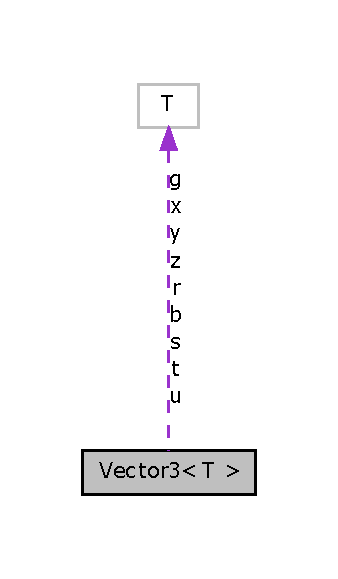
\includegraphics[width=162pt]{class_vector3__coll__graph}
\end{center}
\end{figure}
\subsection*{Public Member Functions}
\begin{DoxyCompactItemize}
\item 
\hyperlink{class_vector3_a54f99f4211298d5245ea578bdd5143cc}{Vector3} ()
\begin{DoxyCompactList}\small\item\em Creates and sets to (0,0,0). \item\end{DoxyCompactList}\item 
\hyperlink{class_vector3_af2877fe01d7847181d33860005c4c1eb}{Vector3} (T nx, T ny, T nz)
\begin{DoxyCompactList}\small\item\em Creates and sets to (x,y,z). \item\end{DoxyCompactList}\item 
\hyperlink{class_vector3_aa2fec2c441bba344389faf2a5365079e}{Vector3} (const \hyperlink{class_vector3}{Vector3}$<$ T $>$ \&src)
\begin{DoxyCompactList}\small\item\em Copy constructor. \item\end{DoxyCompactList}\item 
{\footnotesize template$<$class FromT $>$ }\\\hyperlink{class_vector3_aba28547320ba45406511ae1113c8167f}{Vector3} (const \hyperlink{class_vector3}{Vector3}$<$ FromT $>$ \&src)
\begin{DoxyCompactList}\small\item\em Copy casting constructor. \item\end{DoxyCompactList}\item 
\hyperlink{class_vector3}{Vector3}$<$ T $>$ \hyperlink{class_vector3_abe7d8e30be809e8dd0456ac8a3cf4e90}{operator=} (const \hyperlink{class_vector3}{Vector3}$<$ T $>$ \&rhs)
\begin{DoxyCompactList}\small\item\em Copy operator. \item\end{DoxyCompactList}\item 
{\footnotesize template$<$class FromT $>$ }\\\hyperlink{class_vector3}{Vector3}$<$ T $>$ \hyperlink{class_vector3_a84dd48a557067f2ad46ea72f7de6fa3b}{operator=} (const \hyperlink{class_vector3}{Vector3}$<$ FromT $>$ \&rhs)
\begin{DoxyCompactList}\small\item\em Copy casting operator. \item\end{DoxyCompactList}\item 
T \& \hyperlink{class_vector3_aa64b7a8c85eb2f80ee30155e26109a0a}{operator\mbox{[}$\,$\mbox{]}} (int n)
\begin{DoxyCompactList}\small\item\em Array access operator. \item\end{DoxyCompactList}\item 
const T \& \hyperlink{class_vector3_af0a225a033c235384b74377a62630365}{operator\mbox{[}$\,$\mbox{]}} (int n) const 
\begin{DoxyCompactList}\small\item\em Constant array access operator. \item\end{DoxyCompactList}\item 
\hyperlink{class_vector3}{Vector3}$<$ T $>$ \hyperlink{class_vector3_a97c1abe4d4242097f3dcc413277522f5}{operator+} (const \hyperlink{class_vector3}{Vector3}$<$ T $>$ \&rhs) const 
\begin{DoxyCompactList}\small\item\em Addition operator. \item\end{DoxyCompactList}\item 
\hyperlink{class_vector3}{Vector3}$<$ T $>$ \hyperlink{class_vector3_ad6a02e3ed199acf9b74e56639d546a28}{operator-\/} (const \hyperlink{class_vector3}{Vector3}$<$ T $>$ \&rhs) const 
\begin{DoxyCompactList}\small\item\em Subtraction operator. \item\end{DoxyCompactList}\item 
\hyperlink{class_vector3}{Vector3}$<$ T $>$ \hyperlink{class_vector3_a78351785ea5e7a84419a9975301d820c}{operator$\ast$} (const \hyperlink{class_vector3}{Vector3}$<$ T $>$ \&rhs) const 
\begin{DoxyCompactList}\small\item\em Multiplication operator. \item\end{DoxyCompactList}\item 
\hyperlink{class_vector3}{Vector3}$<$ T $>$ \hyperlink{class_vector3_afad9c64ba4b9cbf65ad5c662e4c5fddd}{operator/} (const \hyperlink{class_vector3}{Vector3}$<$ T $>$ \&rhs) const 
\begin{DoxyCompactList}\small\item\em Division operator. \item\end{DoxyCompactList}\item 
\hyperlink{class_vector3}{Vector3}$<$ T $>$ \& \hyperlink{class_vector3_ab50a40b431192f189a9cf0556bcad1c3}{operator+=} (const \hyperlink{class_vector3}{Vector3}$<$ T $>$ \&rhs)
\begin{DoxyCompactList}\small\item\em Addition operator. \item\end{DoxyCompactList}\item 
\hyperlink{class_vector3}{Vector3}$<$ T $>$ \& \hyperlink{class_vector3_ae0bc9179d39a0c80e30c598ffb0639a8}{operator-\/=} (const \hyperlink{class_vector3}{Vector3}$<$ T $>$ \&rhs)
\begin{DoxyCompactList}\small\item\em Subtraction operator. \item\end{DoxyCompactList}\item 
\hyperlink{class_vector3}{Vector3}$<$ T $>$ \& \hyperlink{class_vector3_ab318211043865788f6814e57cc4b6da4}{operator$\ast$=} (const \hyperlink{class_vector3}{Vector3}$<$ T $>$ \&rhs)
\begin{DoxyCompactList}\small\item\em Multiplication operator. \item\end{DoxyCompactList}\item 
\hyperlink{class_vector3}{Vector3}$<$ T $>$ \& \hyperlink{class_vector3_ad0a6161051a0b8bd93c146a0159ce495}{operator/=} (const \hyperlink{class_vector3}{Vector3}$<$ T $>$ \&rhs)
\begin{DoxyCompactList}\small\item\em Division operator. \item\end{DoxyCompactList}\item 
T \hyperlink{class_vector3_a2f1fdf1c794d6337892d5502459d5ccb}{dotProduct} (const \hyperlink{class_vector3}{Vector3}$<$ T $>$ \&rhs) const 
\begin{DoxyCompactList}\small\item\em Dot product of two vectors. \item\end{DoxyCompactList}\item 
\hyperlink{class_vector3}{Vector3}$<$ T $>$ \hyperlink{class_vector3_a75af980b2fd0c531b568ac9cb4021b75}{crossProduct} (const \hyperlink{class_vector3}{Vector3}$<$ T $>$ \&rhs) const 
\begin{DoxyCompactList}\small\item\em Cross product operator. \item\end{DoxyCompactList}\item 
\hyperlink{class_vector3}{Vector3}$<$ T $>$ \hyperlink{class_vector3_a493cc48a44398ad7cc8ad2e056637e80}{operator+} (T rhs) const 
\begin{DoxyCompactList}\small\item\em Addition operator. \item\end{DoxyCompactList}\item 
\hyperlink{class_vector3}{Vector3}$<$ T $>$ \hyperlink{class_vector3_a2cecabf7b0a25697794c320e2c179a42}{operator-\/} (T rhs) const 
\begin{DoxyCompactList}\small\item\em Subtraction operator. \item\end{DoxyCompactList}\item 
\hyperlink{class_vector3}{Vector3}$<$ T $>$ \hyperlink{class_vector3_a413e0c20e64bb1313effc98a4e5f068e}{operator$\ast$} (T rhs) const 
\begin{DoxyCompactList}\small\item\em Multiplication operator. \item\end{DoxyCompactList}\item 
\hyperlink{class_vector3}{Vector3}$<$ T $>$ \hyperlink{class_vector3_a9387fe32c315ff4cdb2b612a72d901d6}{operator/} (T rhs) const 
\begin{DoxyCompactList}\small\item\em Division operator. \item\end{DoxyCompactList}\item 
\hyperlink{class_vector3}{Vector3}$<$ T $>$ \& \hyperlink{class_vector3_a337ea6437958847aeaa7ca761cc9551a}{operator+=} (T rhs)
\begin{DoxyCompactList}\small\item\em Addition operator. \item\end{DoxyCompactList}\item 
\hyperlink{class_vector3}{Vector3}$<$ T $>$ \& \hyperlink{class_vector3_a42c1be3201044a462cfd3115de8fd46e}{operator-\/=} (T rhs)
\begin{DoxyCompactList}\small\item\em Subtraction operator. \item\end{DoxyCompactList}\item 
\hyperlink{class_vector3}{Vector3}$<$ T $>$ \& \hyperlink{class_vector3_a34e1c1ba70d7cea23639c2e71cd17bd9}{operator$\ast$=} (T rhs)
\begin{DoxyCompactList}\small\item\em Multiplication operator. \item\end{DoxyCompactList}\item 
\hyperlink{class_vector3}{Vector3}$<$ T $>$ \& \hyperlink{class_vector3_ab584b594f28c0bbdea48c973d8725179}{operator/=} (T rhs)
\begin{DoxyCompactList}\small\item\em Division operator. \item\end{DoxyCompactList}\item 
bool \hyperlink{class_vector3_af3335b4d12d144e5d796518e9521936b}{operator==} (const \hyperlink{class_vector3}{Vector3}$<$ T $>$ \&rhs) const 
\begin{DoxyCompactList}\small\item\em Equality test operator. \item\end{DoxyCompactList}\item 
bool \hyperlink{class_vector3_a2b688296e6471b97e1540412a5e6e68c}{operator!=} (const \hyperlink{class_vector3}{Vector3}$<$ T $>$ \&rhs) const 
\begin{DoxyCompactList}\small\item\em Inequality test operator. \item\end{DoxyCompactList}\item 
\hyperlink{class_vector3}{Vector3}$<$ T $>$ \hyperlink{class_vector3_a19ffa959993141f3ad4b249cba47c741}{operator-\/} () const 
\begin{DoxyCompactList}\small\item\em Unary negate operator. \item\end{DoxyCompactList}\item 
T \hyperlink{class_vector3_af8f3e528208b3d7fdae9f40e2841f3bb}{length} () const 
\begin{DoxyCompactList}\small\item\em Get length of vector. \item\end{DoxyCompactList}\item 
T \hyperlink{class_vector3_a750daa261b3ffc5fc3491c31c8bbadd2}{lengthSq} () const 
\begin{DoxyCompactList}\small\item\em Return square of length. \item\end{DoxyCompactList}\item 
void \hyperlink{class_vector3_a9b147a862a1b86ed2e5b735d19da3da1}{normalize} ()
\begin{DoxyCompactList}\small\item\em Normalize vector. \item\end{DoxyCompactList}\item 
void \hyperlink{class_vector3_a1f827732a85e05b2ef2b8f00145fb2af}{rotate} (T ax, T ay, T az)
\begin{DoxyCompactList}\small\item\em Rotate vector around three axis. \item\end{DoxyCompactList}\item 
\hyperlink{class_vector3}{Vector3}$<$ T $>$ \hyperlink{class_vector3_a05d0f18d40f03e9dd98970de80e209f5}{lerp} (T fact, const \hyperlink{class_vector3}{Vector3}$<$ T $>$ \&\hyperlink{class_vector3_add6ab48cc3cc8636e4f043caa8824dff}{r}) const 
\begin{DoxyCompactList}\small\item\em Linear interpolation of two vectors. \item\end{DoxyCompactList}\item 
\hyperlink{class_vector3_a8303ebc00016d1fd5923b94b520b19a4}{operator T $\ast$} ()
\begin{DoxyCompactList}\small\item\em Conversion to pointer operator. \item\end{DoxyCompactList}\item 
\hyperlink{class_vector3_a289fabaf4a3f93c3305f003b4ab85ee5}{operator const T $\ast$} () const 
\begin{DoxyCompactList}\small\item\em Conversion to pointer operator. \item\end{DoxyCompactList}\item 
std::string \hyperlink{class_vector3_ae3819967ed3e79fe402ed4340910b8e4}{toString} () const 
\begin{DoxyCompactList}\small\item\em Gets string representation. \item\end{DoxyCompactList}\end{DoxyCompactItemize}
\subsection*{Public Attributes}
\begin{DoxyCompactItemize}
\item 
\begin{tabbing}
xx\=xx\=xx\=xx\=xx\=xx\=xx\=xx\=xx\=\kill
union \{\\
\>T \hyperlink{class_vector3_a1a0f7e168c71ca798099f0ba8a444244}{x}\\
\>\>{\em First element of vector, alias for X-\/coordinate. }\\
\>T \hyperlink{class_vector3_a152ee26cfc844e014925dc4bb31d10b0}{s}\\
\>\>{\em First element of vector, alias for S-\/coordinate. }\\
\>T \hyperlink{class_vector3_add6ab48cc3cc8636e4f043caa8824dff}{r}\\
\>\>{\em First element of vector, alias for R-\/coordinate. }\\
\}; \\

\end{tabbing}\item 
\begin{tabbing}
xx\=xx\=xx\=xx\=xx\=xx\=xx\=xx\=xx\=\kill
union \{\\
\>T \hyperlink{class_vector3_a561df88b28e106e337a25bb86554a569}{y}\\
\>\>{\em Second element of vector, alias for Y-\/coordinate. }\\
\>T \hyperlink{class_vector3_a4543c81991a56da65f37a0bba1695c32}{t}\\
\>\>{\em Second element of vector, alias for T-\/coordinate. }\\
\>T \hyperlink{class_vector3_a2cd87f1cae37ddde9a1bc91acfba4b7c}{g}\\
\>\>{\em Second element of vector, alias for G-\/coordinate. }\\
\}; \\

\end{tabbing}\item 
\begin{tabbing}
xx\=xx\=xx\=xx\=xx\=xx\=xx\=xx\=xx\=\kill
union \{\\
\>T \hyperlink{class_vector3_ab3e7f5401dd6e951978bfa746809f74f}{z}\\
\>\>{\em Third element of vector, alias for Z-\/coordinate. }\\
\>T \hyperlink{class_vector3_aca1ce49fc91888da09306f222ff43756}{u}\\
\>\>{\em Third element of vector, alias for U-\/coordinate. }\\
\>T \hyperlink{class_vector3_a5d0fb92a571771b1611e15e0daeb4826}{b}\\
\>\>{\em Third element of vector, alias for B-\/coordinate. }\\
\}; \\

\end{tabbing}\end{DoxyCompactItemize}
\subsection*{Friends}
\begin{DoxyCompactItemize}
\item 
std::ostream \& \hyperlink{class_vector3_a7713cf8239e5a5d748b25a008615ff01}{operator$<$$<$} (std::ostream \&lhs, const \hyperlink{class_vector3}{Vector3}$<$ T $>$ rhs)
\begin{DoxyCompactList}\small\item\em Output to stream operator. \item\end{DoxyCompactList}\end{DoxyCompactItemize}


\subsection{Detailed Description}
\subsubsection*{template$<$class T$>$ class Vector3$<$ T $>$}

Class for three dimensional vector. There are four ways of accessing vector components. Let's have {\ttfamily Vector3f v}, you can either: 
\begin{DoxyItemize}
\item access as position (x,y,z) --- {\ttfamily v.x = v.y = v.z = 1;} 
\item access as texture coordinate (s,t,u) --- {\ttfamily v.s = v.t = v.u = 1;} 
\item access as color (r,g,b) --- {\ttfamily v.r = v.g = v.b = 1;} 
\item access via operator\mbox{[}\mbox{]} --- {\ttfamily v\mbox{[}0\mbox{]} = v\mbox{[}1\mbox{]} = v\mbox{[}2\mbox{]} = 1;} 
\end{DoxyItemize}

\subsection{Constructor \& Destructor Documentation}
\hypertarget{class_vector3_a54f99f4211298d5245ea578bdd5143cc}{
\index{Vector3@{Vector3}!Vector3@{Vector3}}
\index{Vector3@{Vector3}!Vector3@{Vector3}}
\subsubsection[{Vector3}]{\setlength{\rightskip}{0pt plus 5cm}template$<$class T$>$ {\bf Vector3}$<$ T $>$::{\bf Vector3} (
\begin{DoxyParamCaption}
{}
\end{DoxyParamCaption}
)\hspace{0.3cm}{\ttfamily  \mbox{[}inline\mbox{]}}}}
\label{class_vector3_a54f99f4211298d5245ea578bdd5143cc}


Creates and sets to (0,0,0). 

\hypertarget{class_vector3_af2877fe01d7847181d33860005c4c1eb}{
\index{Vector3@{Vector3}!Vector3@{Vector3}}
\index{Vector3@{Vector3}!Vector3@{Vector3}}
\subsubsection[{Vector3}]{\setlength{\rightskip}{0pt plus 5cm}template$<$class T$>$ {\bf Vector3}$<$ T $>$::{\bf Vector3} (
\begin{DoxyParamCaption}
\item[{T}]{ nx, }
\item[{T}]{ ny, }
\item[{T}]{ nz}
\end{DoxyParamCaption}
)\hspace{0.3cm}{\ttfamily  \mbox{[}inline\mbox{]}}}}
\label{class_vector3_af2877fe01d7847181d33860005c4c1eb}


Creates and sets to (x,y,z). 


\begin{DoxyParams}{Parameters}
\item[{\em nx}]initial x-\/coordinate value \item[{\em ny}]initial y-\/coordinate value \item[{\em nz}]initial z-\/coordinate value \end{DoxyParams}
\hypertarget{class_vector3_aa2fec2c441bba344389faf2a5365079e}{
\index{Vector3@{Vector3}!Vector3@{Vector3}}
\index{Vector3@{Vector3}!Vector3@{Vector3}}
\subsubsection[{Vector3}]{\setlength{\rightskip}{0pt plus 5cm}template$<$class T$>$ {\bf Vector3}$<$ T $>$::{\bf Vector3} (
\begin{DoxyParamCaption}
\item[{const {\bf Vector3}$<$ T $>$ \&}]{ src}
\end{DoxyParamCaption}
)\hspace{0.3cm}{\ttfamily  \mbox{[}inline\mbox{]}}}}
\label{class_vector3_aa2fec2c441bba344389faf2a5365079e}


Copy constructor. 


\begin{DoxyParams}{Parameters}
\item[{\em src}]Source of data for new created \hyperlink{class_vector3}{Vector3} instance. \end{DoxyParams}
\hypertarget{class_vector3_aba28547320ba45406511ae1113c8167f}{
\index{Vector3@{Vector3}!Vector3@{Vector3}}
\index{Vector3@{Vector3}!Vector3@{Vector3}}
\subsubsection[{Vector3}]{\setlength{\rightskip}{0pt plus 5cm}template$<$class T$>$ template$<$class FromT $>$ {\bf Vector3}$<$ T $>$::{\bf Vector3} (
\begin{DoxyParamCaption}
\item[{const {\bf Vector3}$<$ FromT $>$ \&}]{ src}
\end{DoxyParamCaption}
)\hspace{0.3cm}{\ttfamily  \mbox{[}inline\mbox{]}}}}
\label{class_vector3_aba28547320ba45406511ae1113c8167f}


Copy casting constructor. 


\begin{DoxyParams}{Parameters}
\item[{\em src}]Source of data for new created \hyperlink{class_vector3}{Vector3} instance. \end{DoxyParams}


\subsection{Member Function Documentation}
\hypertarget{class_vector3_a75af980b2fd0c531b568ac9cb4021b75}{
\index{Vector3@{Vector3}!crossProduct@{crossProduct}}
\index{crossProduct@{crossProduct}!Vector3@{Vector3}}
\subsubsection[{crossProduct}]{\setlength{\rightskip}{0pt plus 5cm}template$<$class T$>$ {\bf Vector3}$<$T$>$ {\bf Vector3}$<$ T $>$::crossProduct (
\begin{DoxyParamCaption}
\item[{const {\bf Vector3}$<$ T $>$ \&}]{ rhs}
\end{DoxyParamCaption}
) const\hspace{0.3cm}{\ttfamily  \mbox{[}inline\mbox{]}}}}
\label{class_vector3_a75af980b2fd0c531b568ac9cb4021b75}


Cross product operator. 


\begin{DoxyParams}{Parameters}
\item[{\em rhs}]Right hand side argument of binary operator. \end{DoxyParams}
\hypertarget{class_vector3_a2f1fdf1c794d6337892d5502459d5ccb}{
\index{Vector3@{Vector3}!dotProduct@{dotProduct}}
\index{dotProduct@{dotProduct}!Vector3@{Vector3}}
\subsubsection[{dotProduct}]{\setlength{\rightskip}{0pt plus 5cm}template$<$class T$>$ T {\bf Vector3}$<$ T $>$::dotProduct (
\begin{DoxyParamCaption}
\item[{const {\bf Vector3}$<$ T $>$ \&}]{ rhs}
\end{DoxyParamCaption}
) const\hspace{0.3cm}{\ttfamily  \mbox{[}inline\mbox{]}}}}
\label{class_vector3_a2f1fdf1c794d6337892d5502459d5ccb}


Dot product of two vectors. 


\begin{DoxyParams}{Parameters}
\item[{\em rhs}]Right hand side argument of binary operator. \end{DoxyParams}
\hypertarget{class_vector3_af8f3e528208b3d7fdae9f40e2841f3bb}{
\index{Vector3@{Vector3}!length@{length}}
\index{length@{length}!Vector3@{Vector3}}
\subsubsection[{length}]{\setlength{\rightskip}{0pt plus 5cm}template$<$class T$>$ T {\bf Vector3}$<$ T $>$::length (
\begin{DoxyParamCaption}
{}
\end{DoxyParamCaption}
) const\hspace{0.3cm}{\ttfamily  \mbox{[}inline\mbox{]}}}}
\label{class_vector3_af8f3e528208b3d7fdae9f40e2841f3bb}


Get length of vector. 

\begin{DoxyReturn}{Returns}
lenght of vector 
\end{DoxyReturn}
\hypertarget{class_vector3_a750daa261b3ffc5fc3491c31c8bbadd2}{
\index{Vector3@{Vector3}!lengthSq@{lengthSq}}
\index{lengthSq@{lengthSq}!Vector3@{Vector3}}
\subsubsection[{lengthSq}]{\setlength{\rightskip}{0pt plus 5cm}template$<$class T$>$ T {\bf Vector3}$<$ T $>$::lengthSq (
\begin{DoxyParamCaption}
{}
\end{DoxyParamCaption}
) const\hspace{0.3cm}{\ttfamily  \mbox{[}inline\mbox{]}}}}
\label{class_vector3_a750daa261b3ffc5fc3491c31c8bbadd2}


Return square of length. 

\begin{DoxyReturn}{Returns}
length $^\wedge$ 2 
\end{DoxyReturn}
\begin{DoxyNote}{Note}
This method is faster then \hyperlink{class_vector3_af8f3e528208b3d7fdae9f40e2841f3bb}{length()}. For comparison of length of two vector can be used just this value, instead of more expensive \hyperlink{class_vector3_af8f3e528208b3d7fdae9f40e2841f3bb}{length()} method. 
\end{DoxyNote}
\hypertarget{class_vector3_a05d0f18d40f03e9dd98970de80e209f5}{
\index{Vector3@{Vector3}!lerp@{lerp}}
\index{lerp@{lerp}!Vector3@{Vector3}}
\subsubsection[{lerp}]{\setlength{\rightskip}{0pt plus 5cm}template$<$class T$>$ {\bf Vector3}$<$T$>$ {\bf Vector3}$<$ T $>$::lerp (
\begin{DoxyParamCaption}
\item[{T}]{ fact, }
\item[{const {\bf Vector3}$<$ T $>$ \&}]{ r}
\end{DoxyParamCaption}
) const\hspace{0.3cm}{\ttfamily  \mbox{[}inline\mbox{]}}}}
\label{class_vector3_a05d0f18d40f03e9dd98970de80e209f5}


Linear interpolation of two vectors. 


\begin{DoxyParams}{Parameters}
\item[{\em fact}]Factor of interpolation. For translation from positon of this vector to vector r, values of factor goes from 0.0 to 1.0. \item[{\em r}]Second Vector for interpolation \end{DoxyParams}
\begin{DoxyNote}{Note}
However values of fact parameter are reasonable only in interval \mbox{[}0.0 , 1.0\mbox{]}, you can pass also values outside of this interval and you can get result (extrapolation?) 
\end{DoxyNote}
\hypertarget{class_vector3_a9b147a862a1b86ed2e5b735d19da3da1}{
\index{Vector3@{Vector3}!normalize@{normalize}}
\index{normalize@{normalize}!Vector3@{Vector3}}
\subsubsection[{normalize}]{\setlength{\rightskip}{0pt plus 5cm}template$<$class T$>$ void {\bf Vector3}$<$ T $>$::normalize (
\begin{DoxyParamCaption}
{}
\end{DoxyParamCaption}
)\hspace{0.3cm}{\ttfamily  \mbox{[}inline\mbox{]}}}}
\label{class_vector3_a9b147a862a1b86ed2e5b735d19da3da1}


Normalize vector. 

\hypertarget{class_vector3_a289fabaf4a3f93c3305f003b4ab85ee5}{
\index{Vector3@{Vector3}!operator const T $\ast$@{operator const T $\ast$}}
\index{operator const T $\ast$@{operator const T $\ast$}!Vector3@{Vector3}}
\subsubsection[{operator const T $\ast$}]{\setlength{\rightskip}{0pt plus 5cm}template$<$class T$>$ {\bf Vector3}$<$ T $>$::operator const T $\ast$ (
\begin{DoxyParamCaption}
{}
\end{DoxyParamCaption}
) const\hspace{0.3cm}{\ttfamily  \mbox{[}inline\mbox{]}}}}
\label{class_vector3_a289fabaf4a3f93c3305f003b4ab85ee5}


Conversion to pointer operator. 

\begin{DoxyReturn}{Returns}
Constant Pointer to internally stored (in management of class Vector3$<$T$>$) used for passing Vector3$<$T$>$ values to gl$\ast$3\mbox{[}fd\mbox{]} functions. 
\end{DoxyReturn}
\hypertarget{class_vector3_a8303ebc00016d1fd5923b94b520b19a4}{
\index{Vector3@{Vector3}!operator T $\ast$@{operator T $\ast$}}
\index{operator T $\ast$@{operator T $\ast$}!Vector3@{Vector3}}
\subsubsection[{operator T $\ast$}]{\setlength{\rightskip}{0pt plus 5cm}template$<$class T$>$ {\bf Vector3}$<$ T $>$::operator T $\ast$ (
\begin{DoxyParamCaption}
{}
\end{DoxyParamCaption}
)\hspace{0.3cm}{\ttfamily  \mbox{[}inline\mbox{]}}}}
\label{class_vector3_a8303ebc00016d1fd5923b94b520b19a4}


Conversion to pointer operator. 

\begin{DoxyReturn}{Returns}
Pointer to internally stored (in management of class Vector3$<$T$>$) used for passing Vector3$<$T$>$ values to gl$\ast$3\mbox{[}fd\mbox{]} functions. 
\end{DoxyReturn}
\hypertarget{class_vector3_a2b688296e6471b97e1540412a5e6e68c}{
\index{Vector3@{Vector3}!operator!=@{operator!=}}
\index{operator!=@{operator!=}!Vector3@{Vector3}}
\subsubsection[{operator!=}]{\setlength{\rightskip}{0pt plus 5cm}template$<$class T$>$ bool {\bf Vector3}$<$ T $>$::operator!= (
\begin{DoxyParamCaption}
\item[{const {\bf Vector3}$<$ T $>$ \&}]{ rhs}
\end{DoxyParamCaption}
) const\hspace{0.3cm}{\ttfamily  \mbox{[}inline\mbox{]}}}}
\label{class_vector3_a2b688296e6471b97e1540412a5e6e68c}


Inequality test operator. 


\begin{DoxyParams}{Parameters}
\item[{\em rhs}]Right hand side argument of binary operator. \end{DoxyParams}
\begin{DoxyReturn}{Returns}
not (lhs == rhs) :-\/P 
\end{DoxyReturn}
\hypertarget{class_vector3_a413e0c20e64bb1313effc98a4e5f068e}{
\index{Vector3@{Vector3}!operator$\ast$@{operator$\ast$}}
\index{operator$\ast$@{operator$\ast$}!Vector3@{Vector3}}
\subsubsection[{operator$\ast$}]{\setlength{\rightskip}{0pt plus 5cm}template$<$class T$>$ {\bf Vector3}$<$T$>$ {\bf Vector3}$<$ T $>$::operator$\ast$ (
\begin{DoxyParamCaption}
\item[{T}]{ rhs}
\end{DoxyParamCaption}
) const\hspace{0.3cm}{\ttfamily  \mbox{[}inline\mbox{]}}}}
\label{class_vector3_a413e0c20e64bb1313effc98a4e5f068e}


Multiplication operator. 


\begin{DoxyParams}{Parameters}
\item[{\em rhs}]Right hand side argument of binary operator. \end{DoxyParams}
\hypertarget{class_vector3_a78351785ea5e7a84419a9975301d820c}{
\index{Vector3@{Vector3}!operator$\ast$@{operator$\ast$}}
\index{operator$\ast$@{operator$\ast$}!Vector3@{Vector3}}
\subsubsection[{operator$\ast$}]{\setlength{\rightskip}{0pt plus 5cm}template$<$class T$>$ {\bf Vector3}$<$T$>$ {\bf Vector3}$<$ T $>$::operator$\ast$ (
\begin{DoxyParamCaption}
\item[{const {\bf Vector3}$<$ T $>$ \&}]{ rhs}
\end{DoxyParamCaption}
) const\hspace{0.3cm}{\ttfamily  \mbox{[}inline\mbox{]}}}}
\label{class_vector3_a78351785ea5e7a84419a9975301d820c}


Multiplication operator. 


\begin{DoxyParams}{Parameters}
\item[{\em rhs}]Right hand side argument of binary operator. \end{DoxyParams}
\hypertarget{class_vector3_ab318211043865788f6814e57cc4b6da4}{
\index{Vector3@{Vector3}!operator$\ast$=@{operator$\ast$=}}
\index{operator$\ast$=@{operator$\ast$=}!Vector3@{Vector3}}
\subsubsection[{operator$\ast$=}]{\setlength{\rightskip}{0pt plus 5cm}template$<$class T$>$ {\bf Vector3}$<$T$>$\& {\bf Vector3}$<$ T $>$::operator$\ast$= (
\begin{DoxyParamCaption}
\item[{const {\bf Vector3}$<$ T $>$ \&}]{ rhs}
\end{DoxyParamCaption}
)\hspace{0.3cm}{\ttfamily  \mbox{[}inline\mbox{]}}}}
\label{class_vector3_ab318211043865788f6814e57cc4b6da4}


Multiplication operator. 


\begin{DoxyParams}{Parameters}
\item[{\em rhs}]Right hand side argument of binary operator. \end{DoxyParams}
\hypertarget{class_vector3_a34e1c1ba70d7cea23639c2e71cd17bd9}{
\index{Vector3@{Vector3}!operator$\ast$=@{operator$\ast$=}}
\index{operator$\ast$=@{operator$\ast$=}!Vector3@{Vector3}}
\subsubsection[{operator$\ast$=}]{\setlength{\rightskip}{0pt plus 5cm}template$<$class T$>$ {\bf Vector3}$<$T$>$\& {\bf Vector3}$<$ T $>$::operator$\ast$= (
\begin{DoxyParamCaption}
\item[{T}]{ rhs}
\end{DoxyParamCaption}
)\hspace{0.3cm}{\ttfamily  \mbox{[}inline\mbox{]}}}}
\label{class_vector3_a34e1c1ba70d7cea23639c2e71cd17bd9}


Multiplication operator. 


\begin{DoxyParams}{Parameters}
\item[{\em rhs}]Right hand side argument of binary operator. \end{DoxyParams}
\hypertarget{class_vector3_a97c1abe4d4242097f3dcc413277522f5}{
\index{Vector3@{Vector3}!operator+@{operator+}}
\index{operator+@{operator+}!Vector3@{Vector3}}
\subsubsection[{operator+}]{\setlength{\rightskip}{0pt plus 5cm}template$<$class T$>$ {\bf Vector3}$<$T$>$ {\bf Vector3}$<$ T $>$::operator+ (
\begin{DoxyParamCaption}
\item[{const {\bf Vector3}$<$ T $>$ \&}]{ rhs}
\end{DoxyParamCaption}
) const\hspace{0.3cm}{\ttfamily  \mbox{[}inline\mbox{]}}}}
\label{class_vector3_a97c1abe4d4242097f3dcc413277522f5}


Addition operator. 


\begin{DoxyParams}{Parameters}
\item[{\em rhs}]Right hand side argument of binary operator. \end{DoxyParams}
\hypertarget{class_vector3_a493cc48a44398ad7cc8ad2e056637e80}{
\index{Vector3@{Vector3}!operator+@{operator+}}
\index{operator+@{operator+}!Vector3@{Vector3}}
\subsubsection[{operator+}]{\setlength{\rightskip}{0pt plus 5cm}template$<$class T$>$ {\bf Vector3}$<$T$>$ {\bf Vector3}$<$ T $>$::operator+ (
\begin{DoxyParamCaption}
\item[{T}]{ rhs}
\end{DoxyParamCaption}
) const\hspace{0.3cm}{\ttfamily  \mbox{[}inline\mbox{]}}}}
\label{class_vector3_a493cc48a44398ad7cc8ad2e056637e80}


Addition operator. 


\begin{DoxyParams}{Parameters}
\item[{\em rhs}]Right hand side argument of binary operator. \end{DoxyParams}
\hypertarget{class_vector3_a337ea6437958847aeaa7ca761cc9551a}{
\index{Vector3@{Vector3}!operator+=@{operator+=}}
\index{operator+=@{operator+=}!Vector3@{Vector3}}
\subsubsection[{operator+=}]{\setlength{\rightskip}{0pt plus 5cm}template$<$class T$>$ {\bf Vector3}$<$T$>$\& {\bf Vector3}$<$ T $>$::operator+= (
\begin{DoxyParamCaption}
\item[{T}]{ rhs}
\end{DoxyParamCaption}
)\hspace{0.3cm}{\ttfamily  \mbox{[}inline\mbox{]}}}}
\label{class_vector3_a337ea6437958847aeaa7ca761cc9551a}


Addition operator. 


\begin{DoxyParams}{Parameters}
\item[{\em rhs}]Right hand side argument of binary operator. \end{DoxyParams}
\hypertarget{class_vector3_ab50a40b431192f189a9cf0556bcad1c3}{
\index{Vector3@{Vector3}!operator+=@{operator+=}}
\index{operator+=@{operator+=}!Vector3@{Vector3}}
\subsubsection[{operator+=}]{\setlength{\rightskip}{0pt plus 5cm}template$<$class T$>$ {\bf Vector3}$<$T$>$\& {\bf Vector3}$<$ T $>$::operator+= (
\begin{DoxyParamCaption}
\item[{const {\bf Vector3}$<$ T $>$ \&}]{ rhs}
\end{DoxyParamCaption}
)\hspace{0.3cm}{\ttfamily  \mbox{[}inline\mbox{]}}}}
\label{class_vector3_ab50a40b431192f189a9cf0556bcad1c3}


Addition operator. 


\begin{DoxyParams}{Parameters}
\item[{\em rhs}]Right hand side argument of binary operator. \end{DoxyParams}
\hypertarget{class_vector3_a2cecabf7b0a25697794c320e2c179a42}{
\index{Vector3@{Vector3}!operator-\/@{operator-\/}}
\index{operator-\/@{operator-\/}!Vector3@{Vector3}}
\subsubsection[{operator-\/}]{\setlength{\rightskip}{0pt plus 5cm}template$<$class T$>$ {\bf Vector3}$<$T$>$ {\bf Vector3}$<$ T $>$::operator-\/ (
\begin{DoxyParamCaption}
\item[{T}]{ rhs}
\end{DoxyParamCaption}
) const\hspace{0.3cm}{\ttfamily  \mbox{[}inline\mbox{]}}}}
\label{class_vector3_a2cecabf7b0a25697794c320e2c179a42}


Subtraction operator. 


\begin{DoxyParams}{Parameters}
\item[{\em rhs}]Right hand side argument of binary operator. \end{DoxyParams}
\hypertarget{class_vector3_a19ffa959993141f3ad4b249cba47c741}{
\index{Vector3@{Vector3}!operator-\/@{operator-\/}}
\index{operator-\/@{operator-\/}!Vector3@{Vector3}}
\subsubsection[{operator-\/}]{\setlength{\rightskip}{0pt plus 5cm}template$<$class T$>$ {\bf Vector3}$<$T$>$ {\bf Vector3}$<$ T $>$::operator-\/ (
\begin{DoxyParamCaption}
{}
\end{DoxyParamCaption}
) const\hspace{0.3cm}{\ttfamily  \mbox{[}inline\mbox{]}}}}
\label{class_vector3_a19ffa959993141f3ad4b249cba47c741}


Unary negate operator. 

\begin{DoxyReturn}{Returns}
negated vector 
\end{DoxyReturn}
\hypertarget{class_vector3_ad6a02e3ed199acf9b74e56639d546a28}{
\index{Vector3@{Vector3}!operator-\/@{operator-\/}}
\index{operator-\/@{operator-\/}!Vector3@{Vector3}}
\subsubsection[{operator-\/}]{\setlength{\rightskip}{0pt plus 5cm}template$<$class T$>$ {\bf Vector3}$<$T$>$ {\bf Vector3}$<$ T $>$::operator-\/ (
\begin{DoxyParamCaption}
\item[{const {\bf Vector3}$<$ T $>$ \&}]{ rhs}
\end{DoxyParamCaption}
) const\hspace{0.3cm}{\ttfamily  \mbox{[}inline\mbox{]}}}}
\label{class_vector3_ad6a02e3ed199acf9b74e56639d546a28}


Subtraction operator. 


\begin{DoxyParams}{Parameters}
\item[{\em rhs}]Right hand side argument of binary operator. \end{DoxyParams}
\hypertarget{class_vector3_a42c1be3201044a462cfd3115de8fd46e}{
\index{Vector3@{Vector3}!operator-\/=@{operator-\/=}}
\index{operator-\/=@{operator-\/=}!Vector3@{Vector3}}
\subsubsection[{operator-\/=}]{\setlength{\rightskip}{0pt plus 5cm}template$<$class T$>$ {\bf Vector3}$<$T$>$\& {\bf Vector3}$<$ T $>$::operator-\/= (
\begin{DoxyParamCaption}
\item[{T}]{ rhs}
\end{DoxyParamCaption}
)\hspace{0.3cm}{\ttfamily  \mbox{[}inline\mbox{]}}}}
\label{class_vector3_a42c1be3201044a462cfd3115de8fd46e}


Subtraction operator. 


\begin{DoxyParams}{Parameters}
\item[{\em rhs}]Right hand side argument of binary operator. \end{DoxyParams}
\hypertarget{class_vector3_ae0bc9179d39a0c80e30c598ffb0639a8}{
\index{Vector3@{Vector3}!operator-\/=@{operator-\/=}}
\index{operator-\/=@{operator-\/=}!Vector3@{Vector3}}
\subsubsection[{operator-\/=}]{\setlength{\rightskip}{0pt plus 5cm}template$<$class T$>$ {\bf Vector3}$<$T$>$\& {\bf Vector3}$<$ T $>$::operator-\/= (
\begin{DoxyParamCaption}
\item[{const {\bf Vector3}$<$ T $>$ \&}]{ rhs}
\end{DoxyParamCaption}
)\hspace{0.3cm}{\ttfamily  \mbox{[}inline\mbox{]}}}}
\label{class_vector3_ae0bc9179d39a0c80e30c598ffb0639a8}


Subtraction operator. 


\begin{DoxyParams}{Parameters}
\item[{\em rhs}]Right hand side argument of binary operator. \end{DoxyParams}
\hypertarget{class_vector3_afad9c64ba4b9cbf65ad5c662e4c5fddd}{
\index{Vector3@{Vector3}!operator/@{operator/}}
\index{operator/@{operator/}!Vector3@{Vector3}}
\subsubsection[{operator/}]{\setlength{\rightskip}{0pt plus 5cm}template$<$class T$>$ {\bf Vector3}$<$T$>$ {\bf Vector3}$<$ T $>$::operator/ (
\begin{DoxyParamCaption}
\item[{const {\bf Vector3}$<$ T $>$ \&}]{ rhs}
\end{DoxyParamCaption}
) const\hspace{0.3cm}{\ttfamily  \mbox{[}inline\mbox{]}}}}
\label{class_vector3_afad9c64ba4b9cbf65ad5c662e4c5fddd}


Division operator. 


\begin{DoxyParams}{Parameters}
\item[{\em rhs}]Right hand side argument of binary operator. \end{DoxyParams}
\hypertarget{class_vector3_a9387fe32c315ff4cdb2b612a72d901d6}{
\index{Vector3@{Vector3}!operator/@{operator/}}
\index{operator/@{operator/}!Vector3@{Vector3}}
\subsubsection[{operator/}]{\setlength{\rightskip}{0pt plus 5cm}template$<$class T$>$ {\bf Vector3}$<$T$>$ {\bf Vector3}$<$ T $>$::operator/ (
\begin{DoxyParamCaption}
\item[{T}]{ rhs}
\end{DoxyParamCaption}
) const\hspace{0.3cm}{\ttfamily  \mbox{[}inline\mbox{]}}}}
\label{class_vector3_a9387fe32c315ff4cdb2b612a72d901d6}


Division operator. 


\begin{DoxyParams}{Parameters}
\item[{\em rhs}]Right hand side argument of binary operator. \end{DoxyParams}
\hypertarget{class_vector3_ab584b594f28c0bbdea48c973d8725179}{
\index{Vector3@{Vector3}!operator/=@{operator/=}}
\index{operator/=@{operator/=}!Vector3@{Vector3}}
\subsubsection[{operator/=}]{\setlength{\rightskip}{0pt plus 5cm}template$<$class T$>$ {\bf Vector3}$<$T$>$\& {\bf Vector3}$<$ T $>$::operator/= (
\begin{DoxyParamCaption}
\item[{T}]{ rhs}
\end{DoxyParamCaption}
)\hspace{0.3cm}{\ttfamily  \mbox{[}inline\mbox{]}}}}
\label{class_vector3_ab584b594f28c0bbdea48c973d8725179}


Division operator. 


\begin{DoxyParams}{Parameters}
\item[{\em rhs}]Right hand side argument of binary operator. \end{DoxyParams}
\hypertarget{class_vector3_ad0a6161051a0b8bd93c146a0159ce495}{
\index{Vector3@{Vector3}!operator/=@{operator/=}}
\index{operator/=@{operator/=}!Vector3@{Vector3}}
\subsubsection[{operator/=}]{\setlength{\rightskip}{0pt plus 5cm}template$<$class T$>$ {\bf Vector3}$<$T$>$\& {\bf Vector3}$<$ T $>$::operator/= (
\begin{DoxyParamCaption}
\item[{const {\bf Vector3}$<$ T $>$ \&}]{ rhs}
\end{DoxyParamCaption}
)\hspace{0.3cm}{\ttfamily  \mbox{[}inline\mbox{]}}}}
\label{class_vector3_ad0a6161051a0b8bd93c146a0159ce495}


Division operator. 


\begin{DoxyParams}{Parameters}
\item[{\em rhs}]Right hand side argument of binary operator. \end{DoxyParams}
\hypertarget{class_vector3_abe7d8e30be809e8dd0456ac8a3cf4e90}{
\index{Vector3@{Vector3}!operator=@{operator=}}
\index{operator=@{operator=}!Vector3@{Vector3}}
\subsubsection[{operator=}]{\setlength{\rightskip}{0pt plus 5cm}template$<$class T$>$ {\bf Vector3}$<$T$>$ {\bf Vector3}$<$ T $>$::operator= (
\begin{DoxyParamCaption}
\item[{const {\bf Vector3}$<$ T $>$ \&}]{ rhs}
\end{DoxyParamCaption}
)\hspace{0.3cm}{\ttfamily  \mbox{[}inline\mbox{]}}}}
\label{class_vector3_abe7d8e30be809e8dd0456ac8a3cf4e90}


Copy operator. 


\begin{DoxyParams}{Parameters}
\item[{\em rhs}]Right hand side argument of binary operator. \end{DoxyParams}
\hypertarget{class_vector3_a84dd48a557067f2ad46ea72f7de6fa3b}{
\index{Vector3@{Vector3}!operator=@{operator=}}
\index{operator=@{operator=}!Vector3@{Vector3}}
\subsubsection[{operator=}]{\setlength{\rightskip}{0pt plus 5cm}template$<$class T$>$ template$<$class FromT $>$ {\bf Vector3}$<$T$>$ {\bf Vector3}$<$ T $>$::operator= (
\begin{DoxyParamCaption}
\item[{const {\bf Vector3}$<$ FromT $>$ \&}]{ rhs}
\end{DoxyParamCaption}
)\hspace{0.3cm}{\ttfamily  \mbox{[}inline\mbox{]}}}}
\label{class_vector3_a84dd48a557067f2ad46ea72f7de6fa3b}


Copy casting operator. 


\begin{DoxyParams}{Parameters}
\item[{\em rhs}]Right hand side argument of binary operator. \end{DoxyParams}
\hypertarget{class_vector3_af3335b4d12d144e5d796518e9521936b}{
\index{Vector3@{Vector3}!operator==@{operator==}}
\index{operator==@{operator==}!Vector3@{Vector3}}
\subsubsection[{operator==}]{\setlength{\rightskip}{0pt plus 5cm}template$<$class T$>$ bool {\bf Vector3}$<$ T $>$::operator== (
\begin{DoxyParamCaption}
\item[{const {\bf Vector3}$<$ T $>$ \&}]{ rhs}
\end{DoxyParamCaption}
) const\hspace{0.3cm}{\ttfamily  \mbox{[}inline\mbox{]}}}}
\label{class_vector3_af3335b4d12d144e5d796518e9521936b}


Equality test operator. 


\begin{DoxyParams}{Parameters}
\item[{\em rhs}]Right hand side argument of binary operator. \end{DoxyParams}
\begin{DoxyNote}{Note}
Test of equality is based of threshold EPSILON value. To be two values equal, must satisfy this condition $|$ lhs.x -\/ rhs.y $|$ $<$ EPSILON, same for y-\/coordinate, and z-\/coordinate. 
\end{DoxyNote}
\hypertarget{class_vector3_aa64b7a8c85eb2f80ee30155e26109a0a}{
\index{Vector3@{Vector3}!operator\mbox{[}\mbox{]}@{operator[]}}
\index{operator\mbox{[}\mbox{]}@{operator[]}!Vector3@{Vector3}}
\subsubsection[{operator[]}]{\setlength{\rightskip}{0pt plus 5cm}template$<$class T$>$ T\& {\bf Vector3}$<$ T $>$::operator\mbox{[}$\,$\mbox{]} (
\begin{DoxyParamCaption}
\item[{int}]{ n}
\end{DoxyParamCaption}
)\hspace{0.3cm}{\ttfamily  \mbox{[}inline\mbox{]}}}}
\label{class_vector3_aa64b7a8c85eb2f80ee30155e26109a0a}


Array access operator. 


\begin{DoxyParams}{Parameters}
\item[{\em n}]Array index \end{DoxyParams}
\begin{DoxyReturn}{Returns}
For n = 0, reference to x coordinate, n = 1 reference to y, else reference to z y coordinate. 
\end{DoxyReturn}
\hypertarget{class_vector3_af0a225a033c235384b74377a62630365}{
\index{Vector3@{Vector3}!operator\mbox{[}\mbox{]}@{operator[]}}
\index{operator\mbox{[}\mbox{]}@{operator[]}!Vector3@{Vector3}}
\subsubsection[{operator[]}]{\setlength{\rightskip}{0pt plus 5cm}template$<$class T$>$ const T\& {\bf Vector3}$<$ T $>$::operator\mbox{[}$\,$\mbox{]} (
\begin{DoxyParamCaption}
\item[{int}]{ n}
\end{DoxyParamCaption}
) const\hspace{0.3cm}{\ttfamily  \mbox{[}inline\mbox{]}}}}
\label{class_vector3_af0a225a033c235384b74377a62630365}


Constant array access operator. 


\begin{DoxyParams}{Parameters}
\item[{\em n}]Array index \end{DoxyParams}
\begin{DoxyReturn}{Returns}
For n = 0, reference to x coordinate, n = 1 reference to y, else reference to z y coordinate. 
\end{DoxyReturn}
\hypertarget{class_vector3_a1f827732a85e05b2ef2b8f00145fb2af}{
\index{Vector3@{Vector3}!rotate@{rotate}}
\index{rotate@{rotate}!Vector3@{Vector3}}
\subsubsection[{rotate}]{\setlength{\rightskip}{0pt plus 5cm}template$<$class T$>$ void {\bf Vector3}$<$ T $>$::rotate (
\begin{DoxyParamCaption}
\item[{T}]{ ax, }
\item[{T}]{ ay, }
\item[{T}]{ az}
\end{DoxyParamCaption}
)\hspace{0.3cm}{\ttfamily  \mbox{[}inline\mbox{]}}}}
\label{class_vector3_a1f827732a85e05b2ef2b8f00145fb2af}


Rotate vector around three axis. 


\begin{DoxyParams}{Parameters}
\item[{\em ax}]Angle (in degrees) to be rotated around X-\/axis. \item[{\em ay}]Angle (in degrees) to be rotated around Y-\/axis. \item[{\em az}]Angle (in degrees) to be rotated around Z-\/axis. \end{DoxyParams}
\hypertarget{class_vector3_ae3819967ed3e79fe402ed4340910b8e4}{
\index{Vector3@{Vector3}!toString@{toString}}
\index{toString@{toString}!Vector3@{Vector3}}
\subsubsection[{toString}]{\setlength{\rightskip}{0pt plus 5cm}template$<$class T$>$ std::string {\bf Vector3}$<$ T $>$::toString (
\begin{DoxyParamCaption}
{}
\end{DoxyParamCaption}
) const\hspace{0.3cm}{\ttfamily  \mbox{[}inline\mbox{]}}}}
\label{class_vector3_ae3819967ed3e79fe402ed4340910b8e4}


Gets string representation. 



\subsection{Friends And Related Function Documentation}
\hypertarget{class_vector3_a7713cf8239e5a5d748b25a008615ff01}{
\index{Vector3@{Vector3}!operator$<$$<$@{operator$<$$<$}}
\index{operator$<$$<$@{operator$<$$<$}!Vector3@{Vector3}}
\subsubsection[{operator$<$$<$}]{\setlength{\rightskip}{0pt plus 5cm}template$<$class T$>$ std::ostream\& operator$<$$<$ (
\begin{DoxyParamCaption}
\item[{std::ostream \&}]{ lhs, }
\item[{const {\bf Vector3}$<$ T $>$}]{ rhs}
\end{DoxyParamCaption}
)\hspace{0.3cm}{\ttfamily  \mbox{[}friend\mbox{]}}}}
\label{class_vector3_a7713cf8239e5a5d748b25a008615ff01}


Output to stream operator. 


\begin{DoxyParams}{Parameters}
\item[{\em lhs}]Left hand side argument of operator (commonly ostream instance). \item[{\em rhs}]Right hand side argument of operator. \end{DoxyParams}
\begin{DoxyReturn}{Returns}
Left hand side argument -\/ the ostream object passed to operator. 
\end{DoxyReturn}


\subsection{Member Data Documentation}
\hypertarget{class_vector3_a7d6d6cb3630e13c2d949088727accbf0}{
\subsubsection[{"@5}]{\setlength{\rightskip}{0pt plus 5cm}union \{ ... \} }}
\label{class_vector3_a7d6d6cb3630e13c2d949088727accbf0}
\hypertarget{class_vector3_a909d7de04b857428afff56ba37cf03c2}{
\subsubsection[{"@7}]{\setlength{\rightskip}{0pt plus 5cm}union \{ ... \} }}
\label{class_vector3_a909d7de04b857428afff56ba37cf03c2}
\hypertarget{class_vector3_a72d53f24e96f0da668f3f2bc97adecd9}{
\subsubsection[{"@9}]{\setlength{\rightskip}{0pt plus 5cm}union \{ ... \} }}
\label{class_vector3_a72d53f24e96f0da668f3f2bc97adecd9}
\hypertarget{class_vector3_a5d0fb92a571771b1611e15e0daeb4826}{
\index{Vector3@{Vector3}!b@{b}}
\index{b@{b}!Vector3@{Vector3}}
\subsubsection[{b}]{\setlength{\rightskip}{0pt plus 5cm}template$<$class T$>$ T {\bf Vector3}$<$ T $>$::{\bf b}}}
\label{class_vector3_a5d0fb92a571771b1611e15e0daeb4826}


Third element of vector, alias for B-\/coordinate. 

For color notation. \hypertarget{class_vector3_a2cd87f1cae37ddde9a1bc91acfba4b7c}{
\index{Vector3@{Vector3}!g@{g}}
\index{g@{g}!Vector3@{Vector3}}
\subsubsection[{g}]{\setlength{\rightskip}{0pt plus 5cm}template$<$class T$>$ T {\bf Vector3}$<$ T $>$::{\bf g}}}
\label{class_vector3_a2cd87f1cae37ddde9a1bc91acfba4b7c}


Second element of vector, alias for G-\/coordinate. 

For color notation. \hypertarget{class_vector3_add6ab48cc3cc8636e4f043caa8824dff}{
\index{Vector3@{Vector3}!r@{r}}
\index{r@{r}!Vector3@{Vector3}}
\subsubsection[{r}]{\setlength{\rightskip}{0pt plus 5cm}template$<$class T$>$ T {\bf Vector3}$<$ T $>$::{\bf r}}}
\label{class_vector3_add6ab48cc3cc8636e4f043caa8824dff}


First element of vector, alias for R-\/coordinate. 

For color notation. \hypertarget{class_vector3_a152ee26cfc844e014925dc4bb31d10b0}{
\index{Vector3@{Vector3}!s@{s}}
\index{s@{s}!Vector3@{Vector3}}
\subsubsection[{s}]{\setlength{\rightskip}{0pt plus 5cm}template$<$class T$>$ T {\bf Vector3}$<$ T $>$::{\bf s}}}
\label{class_vector3_a152ee26cfc844e014925dc4bb31d10b0}


First element of vector, alias for S-\/coordinate. 

For textures notation. \hypertarget{class_vector3_a4543c81991a56da65f37a0bba1695c32}{
\index{Vector3@{Vector3}!t@{t}}
\index{t@{t}!Vector3@{Vector3}}
\subsubsection[{t}]{\setlength{\rightskip}{0pt plus 5cm}template$<$class T$>$ T {\bf Vector3}$<$ T $>$::{\bf t}}}
\label{class_vector3_a4543c81991a56da65f37a0bba1695c32}


Second element of vector, alias for T-\/coordinate. 

For textures notation. \hypertarget{class_vector3_aca1ce49fc91888da09306f222ff43756}{
\index{Vector3@{Vector3}!u@{u}}
\index{u@{u}!Vector3@{Vector3}}
\subsubsection[{u}]{\setlength{\rightskip}{0pt plus 5cm}template$<$class T$>$ T {\bf Vector3}$<$ T $>$::{\bf u}}}
\label{class_vector3_aca1ce49fc91888da09306f222ff43756}


Third element of vector, alias for U-\/coordinate. 

For textures notation. \hypertarget{class_vector3_a1a0f7e168c71ca798099f0ba8a444244}{
\index{Vector3@{Vector3}!x@{x}}
\index{x@{x}!Vector3@{Vector3}}
\subsubsection[{x}]{\setlength{\rightskip}{0pt plus 5cm}template$<$class T$>$ T {\bf Vector3}$<$ T $>$::{\bf x}}}
\label{class_vector3_a1a0f7e168c71ca798099f0ba8a444244}


First element of vector, alias for X-\/coordinate. 

\hypertarget{class_vector3_a561df88b28e106e337a25bb86554a569}{
\index{Vector3@{Vector3}!y@{y}}
\index{y@{y}!Vector3@{Vector3}}
\subsubsection[{y}]{\setlength{\rightskip}{0pt plus 5cm}template$<$class T$>$ T {\bf Vector3}$<$ T $>$::{\bf y}}}
\label{class_vector3_a561df88b28e106e337a25bb86554a569}


Second element of vector, alias for Y-\/coordinate. 

\hypertarget{class_vector3_ab3e7f5401dd6e951978bfa746809f74f}{
\index{Vector3@{Vector3}!z@{z}}
\index{z@{z}!Vector3@{Vector3}}
\subsubsection[{z}]{\setlength{\rightskip}{0pt plus 5cm}template$<$class T$>$ T {\bf Vector3}$<$ T $>$::{\bf z}}}
\label{class_vector3_ab3e7f5401dd6e951978bfa746809f74f}


Third element of vector, alias for Z-\/coordinate. 



The documentation for this class was generated from the following file:\begin{DoxyCompactItemize}
\item 
src/\hyperlink{vmath_8h}{vmath.h}\end{DoxyCompactItemize}

\hypertarget{class_vector4}{
\section{Vector4$<$ T $>$ Class Template Reference}
\label{class_vector4}\index{Vector4@{Vector4}}
}


Class for four dimensional vector.  




{\ttfamily \#include $<$vmath.h$>$}



Collaboration diagram for Vector4$<$ T $>$:
\nopagebreak
\begin{figure}[H]
\begin{center}
\leavevmode
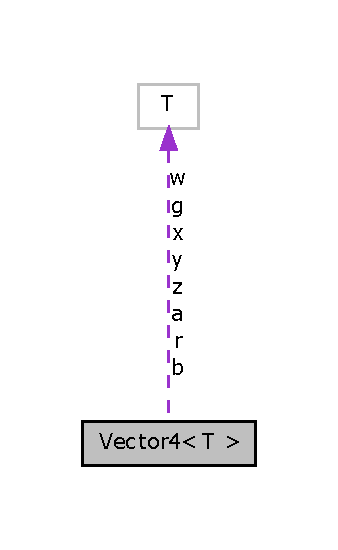
\includegraphics[width=162pt]{class_vector4__coll__graph}
\end{center}
\end{figure}
\subsection*{Public Member Functions}
\begin{DoxyCompactItemize}
\item 
\hyperlink{class_vector4_afdef97d94e5697622b5322637028accf}{Vector4} ()
\begin{DoxyCompactList}\small\item\em Creates and sets to (0,0,0,0). \item\end{DoxyCompactList}\item 
\hyperlink{class_vector4_a6a51b14dfcb4b1bb4b0252f76e602ec8}{Vector4} (T nx, T ny, T nz, T nw)
\begin{DoxyCompactList}\small\item\em Creates and sets to (x,y,z,z). \item\end{DoxyCompactList}\item 
\hyperlink{class_vector4_ae20ddb27878b88964f059495b7311f35}{Vector4} (const \hyperlink{class_vector4}{Vector4}$<$ T $>$ \&src)
\begin{DoxyCompactList}\small\item\em Copy constructor. \item\end{DoxyCompactList}\item 
{\footnotesize template$<$class FromT $>$ }\\\hyperlink{class_vector4_afedec40c43f916ee0951d98c41676a0f}{Vector4} (const \hyperlink{class_vector4}{Vector4}$<$ FromT $>$ \&src)
\begin{DoxyCompactList}\small\item\em Copy casting constructor. \item\end{DoxyCompactList}\item 
\hyperlink{class_vector4}{Vector4}$<$ T $>$ \hyperlink{class_vector4_ace35647d296fb7b9d59083f2a4a7fa7a}{operator=} (const \hyperlink{class_vector4}{Vector4}$<$ T $>$ \&rhs)
\begin{DoxyCompactList}\small\item\em Copy operator. \item\end{DoxyCompactList}\item 
{\footnotesize template$<$class FromT $>$ }\\\hyperlink{class_vector4}{Vector4}$<$ T $>$ \hyperlink{class_vector4_a11f1097f1ff61938d79344f9cd28aad2}{operator=} (const \hyperlink{class_vector4}{Vector4}$<$ FromT $>$ \&rhs)
\begin{DoxyCompactList}\small\item\em Copy casting operator. \item\end{DoxyCompactList}\item 
T \& \hyperlink{class_vector4_a992debdc2a8aee9ba1bcc9bb763a1270}{operator\mbox{[}$\,$\mbox{]}} (int n)
\begin{DoxyCompactList}\small\item\em Array access operator. \item\end{DoxyCompactList}\item 
const T \& \hyperlink{class_vector4_a6ae2a5a65474cb93edc7aceac761850c}{operator\mbox{[}$\,$\mbox{]}} (int n) const 
\begin{DoxyCompactList}\small\item\em Array access operator. \item\end{DoxyCompactList}\item 
\hyperlink{class_vector4}{Vector4}$<$ T $>$ \hyperlink{class_vector4_a80a688fb0462045dd222a0b565477824}{operator+} (const \hyperlink{class_vector4}{Vector4}$<$ T $>$ \&rhs) const 
\begin{DoxyCompactList}\small\item\em Addition operator. \item\end{DoxyCompactList}\item 
\hyperlink{class_vector4}{Vector4}$<$ T $>$ \hyperlink{class_vector4_a46dae2fe0b182172dbc5940ce54329a1}{operator-\/} (const \hyperlink{class_vector4}{Vector4}$<$ T $>$ \&rhs) const 
\begin{DoxyCompactList}\small\item\em Subtraction operator. \item\end{DoxyCompactList}\item 
\hyperlink{class_vector4}{Vector4}$<$ T $>$ \hyperlink{class_vector4_a86f22a427d874dc481b949ed761f9896}{operator$\ast$} (const \hyperlink{class_vector4}{Vector4}$<$ T $>$ rhs) const 
\begin{DoxyCompactList}\small\item\em Multiplication operator. \item\end{DoxyCompactList}\item 
\hyperlink{class_vector4}{Vector4}$<$ T $>$ \hyperlink{class_vector4_ae71f14523d070c119854f1df4c5ee084}{operator/} (const \hyperlink{class_vector4}{Vector4}$<$ T $>$ \&rhs) const 
\begin{DoxyCompactList}\small\item\em Division operator. \item\end{DoxyCompactList}\item 
\hyperlink{class_vector4}{Vector4}$<$ T $>$ \& \hyperlink{class_vector4_abfa5fdfbc2f9569e467e05dd2ecaab26}{operator+=} (const \hyperlink{class_vector4}{Vector4}$<$ T $>$ \&rhs)
\begin{DoxyCompactList}\small\item\em Addition operator. \item\end{DoxyCompactList}\item 
\hyperlink{class_vector4}{Vector4}$<$ T $>$ \& \hyperlink{class_vector4_ad5cfb4045ea0305610179c6bae648520}{operator-\/=} (const \hyperlink{class_vector4}{Vector4}$<$ T $>$ \&rhs)
\begin{DoxyCompactList}\small\item\em Subtraction operator. \item\end{DoxyCompactList}\item 
\hyperlink{class_vector4}{Vector4}$<$ T $>$ \& \hyperlink{class_vector4_a3f5db01486e5265e137a112113cb6cf5}{operator$\ast$=} (const \hyperlink{class_vector4}{Vector4}$<$ T $>$ \&rhs)
\begin{DoxyCompactList}\small\item\em Multiplication operator. \item\end{DoxyCompactList}\item 
\hyperlink{class_vector4}{Vector4}$<$ T $>$ \& \hyperlink{class_vector4_a1dc992e52cfbd78bc502c644dc0521fe}{operator/=} (const \hyperlink{class_vector4}{Vector4}$<$ T $>$ \&rhs)
\begin{DoxyCompactList}\small\item\em Division operator. \item\end{DoxyCompactList}\item 
bool \hyperlink{class_vector4_a2e8f2ec10e407b1f3e731b62c03f8225}{operator==} (const \hyperlink{class_vector4}{Vector4}$<$ T $>$ \&rhs) const 
\begin{DoxyCompactList}\small\item\em Equality test operator. \item\end{DoxyCompactList}\item 
bool \hyperlink{class_vector4_ac31d726332dd8505246ca2360c60300d}{operator!=} (const \hyperlink{class_vector4}{Vector4}$<$ T $>$ \&rhs) const 
\begin{DoxyCompactList}\small\item\em Inequality test operator. \item\end{DoxyCompactList}\item 
\hyperlink{class_vector4}{Vector4}$<$ T $>$ \hyperlink{class_vector4_a7bc7d332788658a92b32694969b4d9e3}{operator-\/} () const 
\begin{DoxyCompactList}\small\item\em Unary negate operator. \item\end{DoxyCompactList}\item 
\hyperlink{class_vector4}{Vector4}$<$ T $>$ \hyperlink{class_vector4_a5004bc94b91923c985e23077cfc937a7}{operator+} (T rhs) const 
\begin{DoxyCompactList}\small\item\em Addition operator. \item\end{DoxyCompactList}\item 
\hyperlink{class_vector4}{Vector4}$<$ T $>$ \hyperlink{class_vector4_addd6c83bcdadd34c0038aae76138aebc}{operator-\/} (T rhs) const 
\begin{DoxyCompactList}\small\item\em Subtraction operator. \item\end{DoxyCompactList}\item 
\hyperlink{class_vector4}{Vector4}$<$ T $>$ \hyperlink{class_vector4_a98e56cc3ef735884b8f70e287ff2ed68}{operator$\ast$} (T rhs) const 
\begin{DoxyCompactList}\small\item\em Multiplication operator. \item\end{DoxyCompactList}\item 
\hyperlink{class_vector4}{Vector4}$<$ T $>$ \hyperlink{class_vector4_a512f5d096b767bcbe1618f01d5a2bebf}{operator/} (T rhs) const 
\begin{DoxyCompactList}\small\item\em Division operator. \item\end{DoxyCompactList}\item 
\hyperlink{class_vector4}{Vector4}$<$ T $>$ \& \hyperlink{class_vector4_a7d465ec9eaffaa3308c4a6c64f2ded8f}{operator+=} (T rhs)
\begin{DoxyCompactList}\small\item\em Addition operator. \item\end{DoxyCompactList}\item 
\hyperlink{class_vector4}{Vector4}$<$ T $>$ \& \hyperlink{class_vector4_a908ced73c807151645080dc7bb9f8516}{operator-\/=} (T rhs)
\begin{DoxyCompactList}\small\item\em Subtraction operator. \item\end{DoxyCompactList}\item 
\hyperlink{class_vector4}{Vector4}$<$ T $>$ \& \hyperlink{class_vector4_a1caac7a97dae951da9039049c93db73f}{operator$\ast$=} (T rhs)
\begin{DoxyCompactList}\small\item\em Multiplication operator. \item\end{DoxyCompactList}\item 
\hyperlink{class_vector4}{Vector4}$<$ T $>$ \& \hyperlink{class_vector4_a2355ed974eac90e81de045dbf522b433}{operator/=} (T rhs)
\begin{DoxyCompactList}\small\item\em Division operator. \item\end{DoxyCompactList}\item 
T \hyperlink{class_vector4_a2242e63f194ec1a46efaae9417f3593c}{length} () const 
\begin{DoxyCompactList}\small\item\em Get length of vector. \item\end{DoxyCompactList}\item 
void \hyperlink{class_vector4_a854ae5d3ecf13efd5251a1e32c43f1b3}{normalize} ()
\begin{DoxyCompactList}\small\item\em Normalize vector. \item\end{DoxyCompactList}\item 
T \hyperlink{class_vector4_a32ac452a5ba86aaf90a3d75709990f0c}{lengthSq} () const 
\begin{DoxyCompactList}\small\item\em Return square of length. \item\end{DoxyCompactList}\item 
\hyperlink{class_vector4}{Vector4}$<$ T $>$ \hyperlink{class_vector4_a59a2b76485334331aa3a2759f3ff45b0}{lerp} (T fact, const \hyperlink{class_vector4}{Vector4}$<$ T $>$ \&\hyperlink{class_vector4_add0f79fe4a8f6d4e1d2aadb2f0c9bbdd}{r}) const 
\begin{DoxyCompactList}\small\item\em Linear interpolation of two vectors. \item\end{DoxyCompactList}\item 
\hyperlink{class_vector4_ac7f1f6e3b48b7878434200d7f2ff035c}{operator T $\ast$} ()
\begin{DoxyCompactList}\small\item\em Conversion to pointer operator. \item\end{DoxyCompactList}\item 
\hyperlink{class_vector4_a6bd576e3ee44ba853b2c8f854a237b2e}{operator const T $\ast$} () const 
\begin{DoxyCompactList}\small\item\em Conversion to pointer operator. \item\end{DoxyCompactList}\item 
std::string \hyperlink{class_vector4_af3ca83cdb1ee34545c18707232dfbc3d}{toString} () const 
\begin{DoxyCompactList}\small\item\em Gets string representation. \item\end{DoxyCompactList}\end{DoxyCompactItemize}
\subsection*{Public Attributes}
\begin{DoxyCompactItemize}
\item 
\begin{tabbing}
xx\=xx\=xx\=xx\=xx\=xx\=xx\=xx\=xx\=\kill
union \{\\
\>T \hyperlink{class_vector4_add0f79fe4a8f6d4e1d2aadb2f0c9bbdd}{r}\\
\>\>{\em First element of vector, alias for R-\/coordinate. }\\
\>T \hyperlink{class_vector4_a2cedf20d2f695a4f0254681b13311ac9}{x}\\
\}; \\

\end{tabbing}\item 
\begin{tabbing}
xx\=xx\=xx\=xx\=xx\=xx\=xx\=xx\=xx\=\kill
union \{\\
\>T \hyperlink{class_vector4_acd9cbf0e72286a325f50793cab3d94e0}{g}\\
\>\>{\em Second element of vector, alias for G-\/coordinate. }\\
\>T \hyperlink{class_vector4_aad001ba27515dc2dcb921e9c83596520}{y}\\
\>\>{\em Second element of vector, alias for Y-\/coordinate. }\\
\}; \\

\end{tabbing}\item 
\begin{tabbing}
xx\=xx\=xx\=xx\=xx\=xx\=xx\=xx\=xx\=\kill
union \{\\
\>T \hyperlink{class_vector4_a147df940f8e570124eb54226be07f28b}{b}\\
\>\>{\em Third element of vector, alias for B-\/coordinate. }\\
\>T \hyperlink{class_vector4_a5a7a1452d661e0b24e4b04c4dbff8ae7}{z}\\
\>\>{\em Third element of vector, alias for Z-\/coordinate. }\\
\}; \\

\end{tabbing}\item 
\begin{tabbing}
xx\=xx\=xx\=xx\=xx\=xx\=xx\=xx\=xx\=\kill
union \{\\
\>T \hyperlink{class_vector4_a32a0b541c80b0eb5c2c08634b7ab4e3b}{a}\\
\>\>{\em Fourth element of vector, alias for A-\/coordinate. }\\
\>T \hyperlink{class_vector4_a83daff43fa2b88b4e76474f4b9a45276}{w}\\
\>\>{\em First element of vector, alias for W-\/coordinate. }\\
\}; \\

\end{tabbing}\end{DoxyCompactItemize}
\subsection*{Friends}
\begin{DoxyCompactItemize}
\item 
std::ostream \& \hyperlink{class_vector4_acaeb205c81fccf7c59d96e13f1af1a21}{operator$<$$<$} (std::ostream \&lhs, const \hyperlink{class_vector4}{Vector4}$<$ T $>$ \&rhs)
\begin{DoxyCompactList}\small\item\em Output to stream operator. \item\end{DoxyCompactList}\end{DoxyCompactItemize}


\subsection{Detailed Description}
\subsubsection*{template$<$class T$>$ class Vector4$<$ T $>$}

Class for four dimensional vector. There are four ways of accessing vector components. Let's have {\ttfamily Vector4f v}, you can either: 
\begin{DoxyItemize}
\item access as position in projective space (x,y,z,w) --- {\ttfamily v.x = v.y = v.z = v.w = 1;} 
\item access as texture coordinate (s,t,u,v) --- {\ttfamily v.s = v.t = v.u = v.v = 1;} 
\item access as color (r,g,b,a) --- {\ttfamily v.r = v.g = v.b = v.a = 1;} 
\item access via operator\mbox{[}\mbox{]} --- {\ttfamily v\mbox{[}0\mbox{]} = v\mbox{[}1\mbox{]} = v\mbox{[}2\mbox{]} = v\mbox{[}3\mbox{]} = 1;} 
\end{DoxyItemize}

\subsection{Constructor \& Destructor Documentation}
\hypertarget{class_vector4_afdef97d94e5697622b5322637028accf}{
\index{Vector4@{Vector4}!Vector4@{Vector4}}
\index{Vector4@{Vector4}!Vector4@{Vector4}}
\subsubsection[{Vector4}]{\setlength{\rightskip}{0pt plus 5cm}template$<$class T$>$ {\bf Vector4}$<$ T $>$::{\bf Vector4} (
\begin{DoxyParamCaption}
{}
\end{DoxyParamCaption}
)\hspace{0.3cm}{\ttfamily  \mbox{[}inline\mbox{]}}}}
\label{class_vector4_afdef97d94e5697622b5322637028accf}


Creates and sets to (0,0,0,0). 

\hypertarget{class_vector4_a6a51b14dfcb4b1bb4b0252f76e602ec8}{
\index{Vector4@{Vector4}!Vector4@{Vector4}}
\index{Vector4@{Vector4}!Vector4@{Vector4}}
\subsubsection[{Vector4}]{\setlength{\rightskip}{0pt plus 5cm}template$<$class T$>$ {\bf Vector4}$<$ T $>$::{\bf Vector4} (
\begin{DoxyParamCaption}
\item[{T}]{ nx, }
\item[{T}]{ ny, }
\item[{T}]{ nz, }
\item[{T}]{ nw}
\end{DoxyParamCaption}
)\hspace{0.3cm}{\ttfamily  \mbox{[}inline\mbox{]}}}}
\label{class_vector4_a6a51b14dfcb4b1bb4b0252f76e602ec8}


Creates and sets to (x,y,z,z). 


\begin{DoxyParams}{Parameters}
\item[{\em nx}]initial x-\/coordinate value (R) \item[{\em ny}]initial y-\/coordinate value (G) \item[{\em nz}]initial z-\/coordinate value (B) \item[{\em nw}]initial w-\/coordinate value (Alpha) \end{DoxyParams}
\hypertarget{class_vector4_ae20ddb27878b88964f059495b7311f35}{
\index{Vector4@{Vector4}!Vector4@{Vector4}}
\index{Vector4@{Vector4}!Vector4@{Vector4}}
\subsubsection[{Vector4}]{\setlength{\rightskip}{0pt plus 5cm}template$<$class T$>$ {\bf Vector4}$<$ T $>$::{\bf Vector4} (
\begin{DoxyParamCaption}
\item[{const {\bf Vector4}$<$ T $>$ \&}]{ src}
\end{DoxyParamCaption}
)\hspace{0.3cm}{\ttfamily  \mbox{[}inline\mbox{]}}}}
\label{class_vector4_ae20ddb27878b88964f059495b7311f35}


Copy constructor. 


\begin{DoxyParams}{Parameters}
\item[{\em src}]Source of data for new created \hyperlink{class_vector4}{Vector4} instance. \end{DoxyParams}
\hypertarget{class_vector4_afedec40c43f916ee0951d98c41676a0f}{
\index{Vector4@{Vector4}!Vector4@{Vector4}}
\index{Vector4@{Vector4}!Vector4@{Vector4}}
\subsubsection[{Vector4}]{\setlength{\rightskip}{0pt plus 5cm}template$<$class T$>$ template$<$class FromT $>$ {\bf Vector4}$<$ T $>$::{\bf Vector4} (
\begin{DoxyParamCaption}
\item[{const {\bf Vector4}$<$ FromT $>$ \&}]{ src}
\end{DoxyParamCaption}
)\hspace{0.3cm}{\ttfamily  \mbox{[}inline\mbox{]}}}}
\label{class_vector4_afedec40c43f916ee0951d98c41676a0f}


Copy casting constructor. 


\begin{DoxyParams}{Parameters}
\item[{\em src}]Source of data for new created \hyperlink{class_vector4}{Vector4} instance. \end{DoxyParams}


\subsection{Member Function Documentation}
\hypertarget{class_vector4_a2242e63f194ec1a46efaae9417f3593c}{
\index{Vector4@{Vector4}!length@{length}}
\index{length@{length}!Vector4@{Vector4}}
\subsubsection[{length}]{\setlength{\rightskip}{0pt plus 5cm}template$<$class T$>$ T {\bf Vector4}$<$ T $>$::length (
\begin{DoxyParamCaption}
{}
\end{DoxyParamCaption}
) const\hspace{0.3cm}{\ttfamily  \mbox{[}inline\mbox{]}}}}
\label{class_vector4_a2242e63f194ec1a46efaae9417f3593c}


Get length of vector. 

\begin{DoxyReturn}{Returns}
lenght of vector 
\end{DoxyReturn}
\hypertarget{class_vector4_a32ac452a5ba86aaf90a3d75709990f0c}{
\index{Vector4@{Vector4}!lengthSq@{lengthSq}}
\index{lengthSq@{lengthSq}!Vector4@{Vector4}}
\subsubsection[{lengthSq}]{\setlength{\rightskip}{0pt plus 5cm}template$<$class T$>$ T {\bf Vector4}$<$ T $>$::lengthSq (
\begin{DoxyParamCaption}
{}
\end{DoxyParamCaption}
) const\hspace{0.3cm}{\ttfamily  \mbox{[}inline\mbox{]}}}}
\label{class_vector4_a32ac452a5ba86aaf90a3d75709990f0c}


Return square of length. 

\begin{DoxyReturn}{Returns}
length $^\wedge$ 2 
\end{DoxyReturn}
\begin{DoxyNote}{Note}
This method is faster then \hyperlink{class_vector4_a2242e63f194ec1a46efaae9417f3593c}{length()}. For comparison of length of two vector can be used just this value, instead of more expensive \hyperlink{class_vector4_a2242e63f194ec1a46efaae9417f3593c}{length()} method. 
\end{DoxyNote}
\hypertarget{class_vector4_a59a2b76485334331aa3a2759f3ff45b0}{
\index{Vector4@{Vector4}!lerp@{lerp}}
\index{lerp@{lerp}!Vector4@{Vector4}}
\subsubsection[{lerp}]{\setlength{\rightskip}{0pt plus 5cm}template$<$class T$>$ {\bf Vector4}$<$T$>$ {\bf Vector4}$<$ T $>$::lerp (
\begin{DoxyParamCaption}
\item[{T}]{ fact, }
\item[{const {\bf Vector4}$<$ T $>$ \&}]{ r}
\end{DoxyParamCaption}
) const\hspace{0.3cm}{\ttfamily  \mbox{[}inline\mbox{]}}}}
\label{class_vector4_a59a2b76485334331aa3a2759f3ff45b0}


Linear interpolation of two vectors. 


\begin{DoxyParams}{Parameters}
\item[{\em fact}]Factor of interpolation. For translation from position of this vector to vector r, values of factor goes from 0.0 to 1.0. \item[{\em r}]Second Vector for interpolation \end{DoxyParams}
\begin{DoxyNote}{Note}
However values of fact parameter are reasonable only in interval \mbox{[}0.0 , 1.0\mbox{]}, you can pass also values outside of this interval and you can get result (extrapolation?) 
\end{DoxyNote}
\hypertarget{class_vector4_a854ae5d3ecf13efd5251a1e32c43f1b3}{
\index{Vector4@{Vector4}!normalize@{normalize}}
\index{normalize@{normalize}!Vector4@{Vector4}}
\subsubsection[{normalize}]{\setlength{\rightskip}{0pt plus 5cm}template$<$class T$>$ void {\bf Vector4}$<$ T $>$::normalize (
\begin{DoxyParamCaption}
{}
\end{DoxyParamCaption}
)\hspace{0.3cm}{\ttfamily  \mbox{[}inline\mbox{]}}}}
\label{class_vector4_a854ae5d3ecf13efd5251a1e32c43f1b3}


Normalize vector. 

\hypertarget{class_vector4_a6bd576e3ee44ba853b2c8f854a237b2e}{
\index{Vector4@{Vector4}!operator const T $\ast$@{operator const T $\ast$}}
\index{operator const T $\ast$@{operator const T $\ast$}!Vector4@{Vector4}}
\subsubsection[{operator const T $\ast$}]{\setlength{\rightskip}{0pt plus 5cm}template$<$class T$>$ {\bf Vector4}$<$ T $>$::operator const T $\ast$ (
\begin{DoxyParamCaption}
{}
\end{DoxyParamCaption}
) const\hspace{0.3cm}{\ttfamily  \mbox{[}inline\mbox{]}}}}
\label{class_vector4_a6bd576e3ee44ba853b2c8f854a237b2e}


Conversion to pointer operator. 

\begin{DoxyReturn}{Returns}
Constant Pointer to internally stored (in management of class Vector4$<$T$>$) used for passing Vector4$<$T$>$ values to gl$\ast$4\mbox{[}fd\mbox{]} functions. 
\end{DoxyReturn}
\hypertarget{class_vector4_ac7f1f6e3b48b7878434200d7f2ff035c}{
\index{Vector4@{Vector4}!operator T $\ast$@{operator T $\ast$}}
\index{operator T $\ast$@{operator T $\ast$}!Vector4@{Vector4}}
\subsubsection[{operator T $\ast$}]{\setlength{\rightskip}{0pt plus 5cm}template$<$class T$>$ {\bf Vector4}$<$ T $>$::operator T $\ast$ (
\begin{DoxyParamCaption}
{}
\end{DoxyParamCaption}
)\hspace{0.3cm}{\ttfamily  \mbox{[}inline\mbox{]}}}}
\label{class_vector4_ac7f1f6e3b48b7878434200d7f2ff035c}


Conversion to pointer operator. 

\begin{DoxyReturn}{Returns}
Pointer to internally stored (in management of class Vector4$<$T$>$) used for passing Vector4$<$T$>$ values to gl$\ast$4\mbox{[}fd\mbox{]} functions. 
\end{DoxyReturn}
\hypertarget{class_vector4_ac31d726332dd8505246ca2360c60300d}{
\index{Vector4@{Vector4}!operator!=@{operator!=}}
\index{operator!=@{operator!=}!Vector4@{Vector4}}
\subsubsection[{operator!=}]{\setlength{\rightskip}{0pt plus 5cm}template$<$class T$>$ bool {\bf Vector4}$<$ T $>$::operator!= (
\begin{DoxyParamCaption}
\item[{const {\bf Vector4}$<$ T $>$ \&}]{ rhs}
\end{DoxyParamCaption}
) const\hspace{0.3cm}{\ttfamily  \mbox{[}inline\mbox{]}}}}
\label{class_vector4_ac31d726332dd8505246ca2360c60300d}


Inequality test operator. 


\begin{DoxyParams}{Parameters}
\item[{\em rhs}]Right hand side argument of binary operator. \end{DoxyParams}
\begin{DoxyReturn}{Returns}
not (lhs == rhs) :-\/P 
\end{DoxyReturn}
\hypertarget{class_vector4_a98e56cc3ef735884b8f70e287ff2ed68}{
\index{Vector4@{Vector4}!operator$\ast$@{operator$\ast$}}
\index{operator$\ast$@{operator$\ast$}!Vector4@{Vector4}}
\subsubsection[{operator$\ast$}]{\setlength{\rightskip}{0pt plus 5cm}template$<$class T$>$ {\bf Vector4}$<$T$>$ {\bf Vector4}$<$ T $>$::operator$\ast$ (
\begin{DoxyParamCaption}
\item[{T}]{ rhs}
\end{DoxyParamCaption}
) const\hspace{0.3cm}{\ttfamily  \mbox{[}inline\mbox{]}}}}
\label{class_vector4_a98e56cc3ef735884b8f70e287ff2ed68}


Multiplication operator. 


\begin{DoxyParams}{Parameters}
\item[{\em rhs}]Right hand side argument of binary operator. \end{DoxyParams}
\hypertarget{class_vector4_a86f22a427d874dc481b949ed761f9896}{
\index{Vector4@{Vector4}!operator$\ast$@{operator$\ast$}}
\index{operator$\ast$@{operator$\ast$}!Vector4@{Vector4}}
\subsubsection[{operator$\ast$}]{\setlength{\rightskip}{0pt plus 5cm}template$<$class T$>$ {\bf Vector4}$<$T$>$ {\bf Vector4}$<$ T $>$::operator$\ast$ (
\begin{DoxyParamCaption}
\item[{const {\bf Vector4}$<$ T $>$}]{ rhs}
\end{DoxyParamCaption}
) const\hspace{0.3cm}{\ttfamily  \mbox{[}inline\mbox{]}}}}
\label{class_vector4_a86f22a427d874dc481b949ed761f9896}


Multiplication operator. 


\begin{DoxyParams}{Parameters}
\item[{\em rhs}]Right hand side argument of binary operator. \end{DoxyParams}
\hypertarget{class_vector4_a3f5db01486e5265e137a112113cb6cf5}{
\index{Vector4@{Vector4}!operator$\ast$=@{operator$\ast$=}}
\index{operator$\ast$=@{operator$\ast$=}!Vector4@{Vector4}}
\subsubsection[{operator$\ast$=}]{\setlength{\rightskip}{0pt plus 5cm}template$<$class T$>$ {\bf Vector4}$<$T$>$\& {\bf Vector4}$<$ T $>$::operator$\ast$= (
\begin{DoxyParamCaption}
\item[{const {\bf Vector4}$<$ T $>$ \&}]{ rhs}
\end{DoxyParamCaption}
)\hspace{0.3cm}{\ttfamily  \mbox{[}inline\mbox{]}}}}
\label{class_vector4_a3f5db01486e5265e137a112113cb6cf5}


Multiplication operator. 


\begin{DoxyParams}{Parameters}
\item[{\em rhs}]Right hand side argument of binary operator. \end{DoxyParams}
\hypertarget{class_vector4_a1caac7a97dae951da9039049c93db73f}{
\index{Vector4@{Vector4}!operator$\ast$=@{operator$\ast$=}}
\index{operator$\ast$=@{operator$\ast$=}!Vector4@{Vector4}}
\subsubsection[{operator$\ast$=}]{\setlength{\rightskip}{0pt plus 5cm}template$<$class T$>$ {\bf Vector4}$<$T$>$\& {\bf Vector4}$<$ T $>$::operator$\ast$= (
\begin{DoxyParamCaption}
\item[{T}]{ rhs}
\end{DoxyParamCaption}
)\hspace{0.3cm}{\ttfamily  \mbox{[}inline\mbox{]}}}}
\label{class_vector4_a1caac7a97dae951da9039049c93db73f}


Multiplication operator. 


\begin{DoxyParams}{Parameters}
\item[{\em rhs}]Right hand side argument of binary operator. \end{DoxyParams}
\hypertarget{class_vector4_a5004bc94b91923c985e23077cfc937a7}{
\index{Vector4@{Vector4}!operator+@{operator+}}
\index{operator+@{operator+}!Vector4@{Vector4}}
\subsubsection[{operator+}]{\setlength{\rightskip}{0pt plus 5cm}template$<$class T$>$ {\bf Vector4}$<$T$>$ {\bf Vector4}$<$ T $>$::operator+ (
\begin{DoxyParamCaption}
\item[{T}]{ rhs}
\end{DoxyParamCaption}
) const\hspace{0.3cm}{\ttfamily  \mbox{[}inline\mbox{]}}}}
\label{class_vector4_a5004bc94b91923c985e23077cfc937a7}


Addition operator. 


\begin{DoxyParams}{Parameters}
\item[{\em rhs}]Right hand side argument of binary operator. \end{DoxyParams}
\hypertarget{class_vector4_a80a688fb0462045dd222a0b565477824}{
\index{Vector4@{Vector4}!operator+@{operator+}}
\index{operator+@{operator+}!Vector4@{Vector4}}
\subsubsection[{operator+}]{\setlength{\rightskip}{0pt plus 5cm}template$<$class T$>$ {\bf Vector4}$<$T$>$ {\bf Vector4}$<$ T $>$::operator+ (
\begin{DoxyParamCaption}
\item[{const {\bf Vector4}$<$ T $>$ \&}]{ rhs}
\end{DoxyParamCaption}
) const\hspace{0.3cm}{\ttfamily  \mbox{[}inline\mbox{]}}}}
\label{class_vector4_a80a688fb0462045dd222a0b565477824}


Addition operator. 


\begin{DoxyParams}{Parameters}
\item[{\em rhs}]Right hand side argument of binary operator. \end{DoxyParams}
\hypertarget{class_vector4_a7d465ec9eaffaa3308c4a6c64f2ded8f}{
\index{Vector4@{Vector4}!operator+=@{operator+=}}
\index{operator+=@{operator+=}!Vector4@{Vector4}}
\subsubsection[{operator+=}]{\setlength{\rightskip}{0pt plus 5cm}template$<$class T$>$ {\bf Vector4}$<$T$>$\& {\bf Vector4}$<$ T $>$::operator+= (
\begin{DoxyParamCaption}
\item[{T}]{ rhs}
\end{DoxyParamCaption}
)\hspace{0.3cm}{\ttfamily  \mbox{[}inline\mbox{]}}}}
\label{class_vector4_a7d465ec9eaffaa3308c4a6c64f2ded8f}


Addition operator. 


\begin{DoxyParams}{Parameters}
\item[{\em rhs}]Right hand side argument of binary operator. \end{DoxyParams}
\hypertarget{class_vector4_abfa5fdfbc2f9569e467e05dd2ecaab26}{
\index{Vector4@{Vector4}!operator+=@{operator+=}}
\index{operator+=@{operator+=}!Vector4@{Vector4}}
\subsubsection[{operator+=}]{\setlength{\rightskip}{0pt plus 5cm}template$<$class T$>$ {\bf Vector4}$<$T$>$\& {\bf Vector4}$<$ T $>$::operator+= (
\begin{DoxyParamCaption}
\item[{const {\bf Vector4}$<$ T $>$ \&}]{ rhs}
\end{DoxyParamCaption}
)\hspace{0.3cm}{\ttfamily  \mbox{[}inline\mbox{]}}}}
\label{class_vector4_abfa5fdfbc2f9569e467e05dd2ecaab26}


Addition operator. 


\begin{DoxyParams}{Parameters}
\item[{\em rhs}]Right hand side argument of binary operator. \end{DoxyParams}
\hypertarget{class_vector4_addd6c83bcdadd34c0038aae76138aebc}{
\index{Vector4@{Vector4}!operator-\/@{operator-\/}}
\index{operator-\/@{operator-\/}!Vector4@{Vector4}}
\subsubsection[{operator-\/}]{\setlength{\rightskip}{0pt plus 5cm}template$<$class T$>$ {\bf Vector4}$<$T$>$ {\bf Vector4}$<$ T $>$::operator-\/ (
\begin{DoxyParamCaption}
\item[{T}]{ rhs}
\end{DoxyParamCaption}
) const\hspace{0.3cm}{\ttfamily  \mbox{[}inline\mbox{]}}}}
\label{class_vector4_addd6c83bcdadd34c0038aae76138aebc}


Subtraction operator. 


\begin{DoxyParams}{Parameters}
\item[{\em rhs}]Right hand side argument of binary operator. \end{DoxyParams}
\hypertarget{class_vector4_a46dae2fe0b182172dbc5940ce54329a1}{
\index{Vector4@{Vector4}!operator-\/@{operator-\/}}
\index{operator-\/@{operator-\/}!Vector4@{Vector4}}
\subsubsection[{operator-\/}]{\setlength{\rightskip}{0pt plus 5cm}template$<$class T$>$ {\bf Vector4}$<$T$>$ {\bf Vector4}$<$ T $>$::operator-\/ (
\begin{DoxyParamCaption}
\item[{const {\bf Vector4}$<$ T $>$ \&}]{ rhs}
\end{DoxyParamCaption}
) const\hspace{0.3cm}{\ttfamily  \mbox{[}inline\mbox{]}}}}
\label{class_vector4_a46dae2fe0b182172dbc5940ce54329a1}


Subtraction operator. 


\begin{DoxyParams}{Parameters}
\item[{\em rhs}]Right hand side argument of binary operator. \end{DoxyParams}
\hypertarget{class_vector4_a7bc7d332788658a92b32694969b4d9e3}{
\index{Vector4@{Vector4}!operator-\/@{operator-\/}}
\index{operator-\/@{operator-\/}!Vector4@{Vector4}}
\subsubsection[{operator-\/}]{\setlength{\rightskip}{0pt plus 5cm}template$<$class T$>$ {\bf Vector4}$<$T$>$ {\bf Vector4}$<$ T $>$::operator-\/ (
\begin{DoxyParamCaption}
{}
\end{DoxyParamCaption}
) const\hspace{0.3cm}{\ttfamily  \mbox{[}inline\mbox{]}}}}
\label{class_vector4_a7bc7d332788658a92b32694969b4d9e3}


Unary negate operator. 

\begin{DoxyReturn}{Returns}
negated vector 
\end{DoxyReturn}
\hypertarget{class_vector4_a908ced73c807151645080dc7bb9f8516}{
\index{Vector4@{Vector4}!operator-\/=@{operator-\/=}}
\index{operator-\/=@{operator-\/=}!Vector4@{Vector4}}
\subsubsection[{operator-\/=}]{\setlength{\rightskip}{0pt plus 5cm}template$<$class T$>$ {\bf Vector4}$<$T$>$\& {\bf Vector4}$<$ T $>$::operator-\/= (
\begin{DoxyParamCaption}
\item[{T}]{ rhs}
\end{DoxyParamCaption}
)\hspace{0.3cm}{\ttfamily  \mbox{[}inline\mbox{]}}}}
\label{class_vector4_a908ced73c807151645080dc7bb9f8516}


Subtraction operator. 


\begin{DoxyParams}{Parameters}
\item[{\em rhs}]Right hand side argument of binary operator. \end{DoxyParams}
\hypertarget{class_vector4_ad5cfb4045ea0305610179c6bae648520}{
\index{Vector4@{Vector4}!operator-\/=@{operator-\/=}}
\index{operator-\/=@{operator-\/=}!Vector4@{Vector4}}
\subsubsection[{operator-\/=}]{\setlength{\rightskip}{0pt plus 5cm}template$<$class T$>$ {\bf Vector4}$<$T$>$\& {\bf Vector4}$<$ T $>$::operator-\/= (
\begin{DoxyParamCaption}
\item[{const {\bf Vector4}$<$ T $>$ \&}]{ rhs}
\end{DoxyParamCaption}
)\hspace{0.3cm}{\ttfamily  \mbox{[}inline\mbox{]}}}}
\label{class_vector4_ad5cfb4045ea0305610179c6bae648520}


Subtraction operator. 


\begin{DoxyParams}{Parameters}
\item[{\em rhs}]Right hand side argument of binary operator. \end{DoxyParams}
\hypertarget{class_vector4_ae71f14523d070c119854f1df4c5ee084}{
\index{Vector4@{Vector4}!operator/@{operator/}}
\index{operator/@{operator/}!Vector4@{Vector4}}
\subsubsection[{operator/}]{\setlength{\rightskip}{0pt plus 5cm}template$<$class T$>$ {\bf Vector4}$<$T$>$ {\bf Vector4}$<$ T $>$::operator/ (
\begin{DoxyParamCaption}
\item[{const {\bf Vector4}$<$ T $>$ \&}]{ rhs}
\end{DoxyParamCaption}
) const\hspace{0.3cm}{\ttfamily  \mbox{[}inline\mbox{]}}}}
\label{class_vector4_ae71f14523d070c119854f1df4c5ee084}


Division operator. 


\begin{DoxyParams}{Parameters}
\item[{\em rhs}]Right hand side argument of binary operator. \end{DoxyParams}
\hypertarget{class_vector4_a512f5d096b767bcbe1618f01d5a2bebf}{
\index{Vector4@{Vector4}!operator/@{operator/}}
\index{operator/@{operator/}!Vector4@{Vector4}}
\subsubsection[{operator/}]{\setlength{\rightskip}{0pt plus 5cm}template$<$class T$>$ {\bf Vector4}$<$T$>$ {\bf Vector4}$<$ T $>$::operator/ (
\begin{DoxyParamCaption}
\item[{T}]{ rhs}
\end{DoxyParamCaption}
) const\hspace{0.3cm}{\ttfamily  \mbox{[}inline\mbox{]}}}}
\label{class_vector4_a512f5d096b767bcbe1618f01d5a2bebf}


Division operator. 


\begin{DoxyParams}{Parameters}
\item[{\em rhs}]Right hand side argument of binary operator. \end{DoxyParams}
\hypertarget{class_vector4_a2355ed974eac90e81de045dbf522b433}{
\index{Vector4@{Vector4}!operator/=@{operator/=}}
\index{operator/=@{operator/=}!Vector4@{Vector4}}
\subsubsection[{operator/=}]{\setlength{\rightskip}{0pt plus 5cm}template$<$class T$>$ {\bf Vector4}$<$T$>$\& {\bf Vector4}$<$ T $>$::operator/= (
\begin{DoxyParamCaption}
\item[{T}]{ rhs}
\end{DoxyParamCaption}
)\hspace{0.3cm}{\ttfamily  \mbox{[}inline\mbox{]}}}}
\label{class_vector4_a2355ed974eac90e81de045dbf522b433}


Division operator. 


\begin{DoxyParams}{Parameters}
\item[{\em rhs}]Right hand side argument of binary operator. \end{DoxyParams}
\hypertarget{class_vector4_a1dc992e52cfbd78bc502c644dc0521fe}{
\index{Vector4@{Vector4}!operator/=@{operator/=}}
\index{operator/=@{operator/=}!Vector4@{Vector4}}
\subsubsection[{operator/=}]{\setlength{\rightskip}{0pt plus 5cm}template$<$class T$>$ {\bf Vector4}$<$T$>$\& {\bf Vector4}$<$ T $>$::operator/= (
\begin{DoxyParamCaption}
\item[{const {\bf Vector4}$<$ T $>$ \&}]{ rhs}
\end{DoxyParamCaption}
)\hspace{0.3cm}{\ttfamily  \mbox{[}inline\mbox{]}}}}
\label{class_vector4_a1dc992e52cfbd78bc502c644dc0521fe}


Division operator. 


\begin{DoxyParams}{Parameters}
\item[{\em rhs}]Right hand side argument of binary operator. \end{DoxyParams}
\hypertarget{class_vector4_a11f1097f1ff61938d79344f9cd28aad2}{
\index{Vector4@{Vector4}!operator=@{operator=}}
\index{operator=@{operator=}!Vector4@{Vector4}}
\subsubsection[{operator=}]{\setlength{\rightskip}{0pt plus 5cm}template$<$class T$>$ template$<$class FromT $>$ {\bf Vector4}$<$T$>$ {\bf Vector4}$<$ T $>$::operator= (
\begin{DoxyParamCaption}
\item[{const {\bf Vector4}$<$ FromT $>$ \&}]{ rhs}
\end{DoxyParamCaption}
)\hspace{0.3cm}{\ttfamily  \mbox{[}inline\mbox{]}}}}
\label{class_vector4_a11f1097f1ff61938d79344f9cd28aad2}


Copy casting operator. 


\begin{DoxyParams}{Parameters}
\item[{\em rhs}]Right hand side argument of binary operator. \end{DoxyParams}
\hypertarget{class_vector4_ace35647d296fb7b9d59083f2a4a7fa7a}{
\index{Vector4@{Vector4}!operator=@{operator=}}
\index{operator=@{operator=}!Vector4@{Vector4}}
\subsubsection[{operator=}]{\setlength{\rightskip}{0pt plus 5cm}template$<$class T$>$ {\bf Vector4}$<$T$>$ {\bf Vector4}$<$ T $>$::operator= (
\begin{DoxyParamCaption}
\item[{const {\bf Vector4}$<$ T $>$ \&}]{ rhs}
\end{DoxyParamCaption}
)\hspace{0.3cm}{\ttfamily  \mbox{[}inline\mbox{]}}}}
\label{class_vector4_ace35647d296fb7b9d59083f2a4a7fa7a}


Copy operator. 


\begin{DoxyParams}{Parameters}
\item[{\em rhs}]Right hand side argument of binary operator. \end{DoxyParams}
\hypertarget{class_vector4_a2e8f2ec10e407b1f3e731b62c03f8225}{
\index{Vector4@{Vector4}!operator==@{operator==}}
\index{operator==@{operator==}!Vector4@{Vector4}}
\subsubsection[{operator==}]{\setlength{\rightskip}{0pt plus 5cm}template$<$class T$>$ bool {\bf Vector4}$<$ T $>$::operator== (
\begin{DoxyParamCaption}
\item[{const {\bf Vector4}$<$ T $>$ \&}]{ rhs}
\end{DoxyParamCaption}
) const\hspace{0.3cm}{\ttfamily  \mbox{[}inline\mbox{]}}}}
\label{class_vector4_a2e8f2ec10e407b1f3e731b62c03f8225}


Equality test operator. 


\begin{DoxyParams}{Parameters}
\item[{\em rhs}]Right hand side argument of binary operator. \end{DoxyParams}
\begin{DoxyNote}{Note}
Test of equality is based of threshold EPSILON value. To be two values equal, must satisfy this condition $|$ lhs.x -\/ rhs.y $|$ $<$ EPSILON, same for y-\/coordinate, z-\/coordinate, and w-\/coordinate. 
\end{DoxyNote}
\hypertarget{class_vector4_a992debdc2a8aee9ba1bcc9bb763a1270}{
\index{Vector4@{Vector4}!operator\mbox{[}\mbox{]}@{operator[]}}
\index{operator\mbox{[}\mbox{]}@{operator[]}!Vector4@{Vector4}}
\subsubsection[{operator[]}]{\setlength{\rightskip}{0pt plus 5cm}template$<$class T$>$ T\& {\bf Vector4}$<$ T $>$::operator\mbox{[}$\,$\mbox{]} (
\begin{DoxyParamCaption}
\item[{int}]{ n}
\end{DoxyParamCaption}
)\hspace{0.3cm}{\ttfamily  \mbox{[}inline\mbox{]}}}}
\label{class_vector4_a992debdc2a8aee9ba1bcc9bb763a1270}


Array access operator. 


\begin{DoxyParams}{Parameters}
\item[{\em n}]Array index \end{DoxyParams}
\begin{DoxyReturn}{Returns}
For n = 0, reference to x coordinate, n = 1 reference to y coordinate, n = 2 reference to z, else reference to w coordinate. 
\end{DoxyReturn}
\hypertarget{class_vector4_a6ae2a5a65474cb93edc7aceac761850c}{
\index{Vector4@{Vector4}!operator\mbox{[}\mbox{]}@{operator[]}}
\index{operator\mbox{[}\mbox{]}@{operator[]}!Vector4@{Vector4}}
\subsubsection[{operator[]}]{\setlength{\rightskip}{0pt plus 5cm}template$<$class T$>$ const T\& {\bf Vector4}$<$ T $>$::operator\mbox{[}$\,$\mbox{]} (
\begin{DoxyParamCaption}
\item[{int}]{ n}
\end{DoxyParamCaption}
) const\hspace{0.3cm}{\ttfamily  \mbox{[}inline\mbox{]}}}}
\label{class_vector4_a6ae2a5a65474cb93edc7aceac761850c}


Array access operator. 


\begin{DoxyParams}{Parameters}
\item[{\em n}]Array index \end{DoxyParams}
\begin{DoxyReturn}{Returns}
For n = 0, reference to x coordinate, n = 1 reference to y coordinate, n = 2 reference to z, else reference to w coordinate. 
\end{DoxyReturn}
\hypertarget{class_vector4_af3ca83cdb1ee34545c18707232dfbc3d}{
\index{Vector4@{Vector4}!toString@{toString}}
\index{toString@{toString}!Vector4@{Vector4}}
\subsubsection[{toString}]{\setlength{\rightskip}{0pt plus 5cm}template$<$class T$>$ std::string {\bf Vector4}$<$ T $>$::toString (
\begin{DoxyParamCaption}
{}
\end{DoxyParamCaption}
) const\hspace{0.3cm}{\ttfamily  \mbox{[}inline\mbox{]}}}}
\label{class_vector4_af3ca83cdb1ee34545c18707232dfbc3d}


Gets string representation. 



\subsection{Friends And Related Function Documentation}
\hypertarget{class_vector4_acaeb205c81fccf7c59d96e13f1af1a21}{
\index{Vector4@{Vector4}!operator$<$$<$@{operator$<$$<$}}
\index{operator$<$$<$@{operator$<$$<$}!Vector4@{Vector4}}
\subsubsection[{operator$<$$<$}]{\setlength{\rightskip}{0pt plus 5cm}template$<$class T$>$ std::ostream\& operator$<$$<$ (
\begin{DoxyParamCaption}
\item[{std::ostream \&}]{ lhs, }
\item[{const {\bf Vector4}$<$ T $>$ \&}]{ rhs}
\end{DoxyParamCaption}
)\hspace{0.3cm}{\ttfamily  \mbox{[}friend\mbox{]}}}}
\label{class_vector4_acaeb205c81fccf7c59d96e13f1af1a21}


Output to stream operator. 


\begin{DoxyParams}{Parameters}
\item[{\em lhs}]Left hand side argument of operator (commonly ostream instance). \item[{\em rhs}]Right hand side argument of operator. \end{DoxyParams}
\begin{DoxyReturn}{Returns}
Left hand side argument -\/ the ostream object passed to operator. 
\end{DoxyReturn}


\subsection{Member Data Documentation}
\hypertarget{class_vector4_a687a777e033b4aeb36745512a285ab15}{
\subsubsection[{"@11}]{\setlength{\rightskip}{0pt plus 5cm}union \{ ... \} }}
\label{class_vector4_a687a777e033b4aeb36745512a285ab15}
\hypertarget{class_vector4_a7c73c2be47abaf5d0e688cc2e09d2a74}{
\subsubsection[{"@13}]{\setlength{\rightskip}{0pt plus 5cm}union \{ ... \} }}
\label{class_vector4_a7c73c2be47abaf5d0e688cc2e09d2a74}
\hypertarget{class_vector4_a7bed48fe8a1f4f4f603ee8124ace6374}{
\subsubsection[{"@15}]{\setlength{\rightskip}{0pt plus 5cm}union \{ ... \} }}
\label{class_vector4_a7bed48fe8a1f4f4f603ee8124ace6374}
\hypertarget{class_vector4_ad6edebc0c1fcc9d21489d1a12fa47ccf}{
\subsubsection[{"@17}]{\setlength{\rightskip}{0pt plus 5cm}union \{ ... \} }}
\label{class_vector4_ad6edebc0c1fcc9d21489d1a12fa47ccf}
\hypertarget{class_vector4_a32a0b541c80b0eb5c2c08634b7ab4e3b}{
\index{Vector4@{Vector4}!a@{a}}
\index{a@{a}!Vector4@{Vector4}}
\subsubsection[{a}]{\setlength{\rightskip}{0pt plus 5cm}template$<$class T$>$ T {\bf Vector4}$<$ T $>$::{\bf a}}}
\label{class_vector4_a32a0b541c80b0eb5c2c08634b7ab4e3b}


Fourth element of vector, alias for A-\/coordinate. 

For color notation. This represnt aplha chanell \hypertarget{class_vector4_a147df940f8e570124eb54226be07f28b}{
\index{Vector4@{Vector4}!b@{b}}
\index{b@{b}!Vector4@{Vector4}}
\subsubsection[{b}]{\setlength{\rightskip}{0pt plus 5cm}template$<$class T$>$ T {\bf Vector4}$<$ T $>$::{\bf b}}}
\label{class_vector4_a147df940f8e570124eb54226be07f28b}


Third element of vector, alias for B-\/coordinate. 

For color notation. \hypertarget{class_vector4_acd9cbf0e72286a325f50793cab3d94e0}{
\index{Vector4@{Vector4}!g@{g}}
\index{g@{g}!Vector4@{Vector4}}
\subsubsection[{g}]{\setlength{\rightskip}{0pt plus 5cm}template$<$class T$>$ T {\bf Vector4}$<$ T $>$::{\bf g}}}
\label{class_vector4_acd9cbf0e72286a325f50793cab3d94e0}


Second element of vector, alias for G-\/coordinate. 

For color notation. \hypertarget{class_vector4_add0f79fe4a8f6d4e1d2aadb2f0c9bbdd}{
\index{Vector4@{Vector4}!r@{r}}
\index{r@{r}!Vector4@{Vector4}}
\subsubsection[{r}]{\setlength{\rightskip}{0pt plus 5cm}template$<$class T$>$ T {\bf Vector4}$<$ T $>$::{\bf r}}}
\label{class_vector4_add0f79fe4a8f6d4e1d2aadb2f0c9bbdd}


First element of vector, alias for R-\/coordinate. 

For color notation. First element of vector, alias for X-\/coordinate. \hypertarget{class_vector4_a83daff43fa2b88b4e76474f4b9a45276}{
\index{Vector4@{Vector4}!w@{w}}
\index{w@{w}!Vector4@{Vector4}}
\subsubsection[{w}]{\setlength{\rightskip}{0pt plus 5cm}template$<$class T$>$ T {\bf Vector4}$<$ T $>$::{\bf w}}}
\label{class_vector4_a83daff43fa2b88b4e76474f4b9a45276}


First element of vector, alias for W-\/coordinate. 

\begin{DoxyNote}{Note}
For vectors (such as normals) should be set to 0.0 For vertices should be set to 1.0 
\end{DoxyNote}
\hypertarget{class_vector4_a2cedf20d2f695a4f0254681b13311ac9}{
\index{Vector4@{Vector4}!x@{x}}
\index{x@{x}!Vector4@{Vector4}}
\subsubsection[{x}]{\setlength{\rightskip}{0pt plus 5cm}template$<$class T$>$ T {\bf Vector4}$<$ T $>$::{\bf x}}}
\label{class_vector4_a2cedf20d2f695a4f0254681b13311ac9}
\hypertarget{class_vector4_aad001ba27515dc2dcb921e9c83596520}{
\index{Vector4@{Vector4}!y@{y}}
\index{y@{y}!Vector4@{Vector4}}
\subsubsection[{y}]{\setlength{\rightskip}{0pt plus 5cm}template$<$class T$>$ T {\bf Vector4}$<$ T $>$::{\bf y}}}
\label{class_vector4_aad001ba27515dc2dcb921e9c83596520}


Second element of vector, alias for Y-\/coordinate. 

\hypertarget{class_vector4_a5a7a1452d661e0b24e4b04c4dbff8ae7}{
\index{Vector4@{Vector4}!z@{z}}
\index{z@{z}!Vector4@{Vector4}}
\subsubsection[{z}]{\setlength{\rightskip}{0pt plus 5cm}template$<$class T$>$ T {\bf Vector4}$<$ T $>$::{\bf z}}}
\label{class_vector4_a5a7a1452d661e0b24e4b04c4dbff8ae7}


Third element of vector, alias for Z-\/coordinate. 



The documentation for this class was generated from the following file:\begin{DoxyCompactItemize}
\item 
src/\hyperlink{vmath_8h}{vmath.h}\end{DoxyCompactItemize}

\chapter{File Documentation}
\hypertarget{vmath_8cpp}{
\section{src/vmath.cpp File Reference}
\label{vmath_8cpp}\index{src/vmath.cpp@{src/vmath.cpp}}
}
{\ttfamily \#include \char`\"{}vmath.h\char`\"{}}\par
Include dependency graph for vmath.cpp:
\nopagebreak
\begin{figure}[H]
\begin{center}
\leavevmode
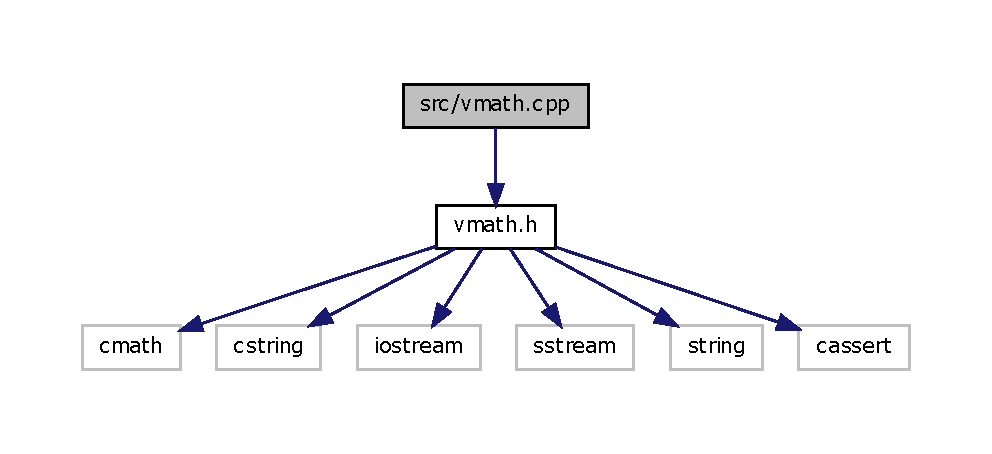
\includegraphics[width=400pt]{vmath_8cpp__incl}
\end{center}
\end{figure}

\hypertarget{vmath_8h}{
\section{src/vmath.h File Reference}
\label{vmath_8h}\index{src/vmath.h@{src/vmath.h}}
}
{\ttfamily \#include $<$cmath$>$}\par
{\ttfamily \#include $<$cstring$>$}\par
{\ttfamily \#include $<$iostream$>$}\par
{\ttfamily \#include $<$sstream$>$}\par
{\ttfamily \#include $<$string$>$}\par
{\ttfamily \#include $<$cassert$>$}\par
Include dependency graph for vmath.h:
\nopagebreak
\begin{figure}[H]
\begin{center}
\leavevmode
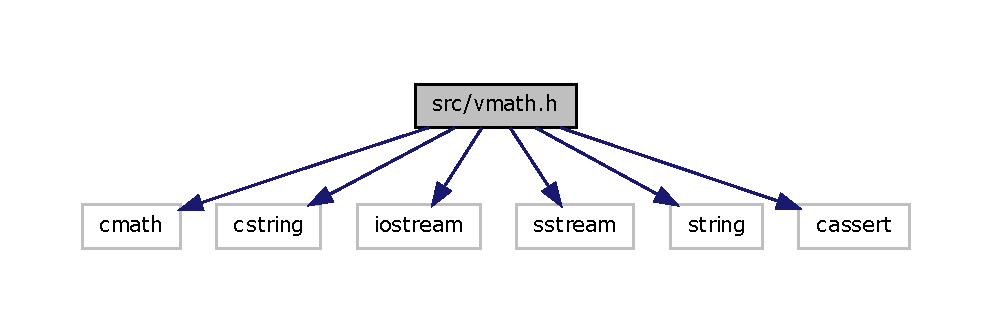
\includegraphics[width=400pt]{vmath_8h__incl}
\end{center}
\end{figure}
This graph shows which files directly or indirectly include this file:
\nopagebreak
\begin{figure}[H]
\begin{center}
\leavevmode
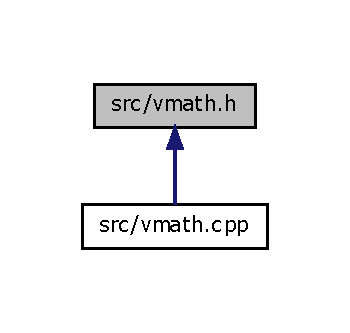
\includegraphics[width=168pt]{vmath_8h__dep__incl}
\end{center}
\end{figure}
\subsection*{Classes}
\begin{DoxyCompactItemize}
\item 
class \hyperlink{class_vector2}{Vector2$<$ T $>$}
\begin{DoxyCompactList}\small\item\em Class for two dimensional vector. \item\end{DoxyCompactList}\item 
class \hyperlink{class_vector3}{Vector3$<$ T $>$}
\begin{DoxyCompactList}\small\item\em Class for three dimensional vector. \item\end{DoxyCompactList}\item 
class \hyperlink{class_vector4}{Vector4$<$ T $>$}
\begin{DoxyCompactList}\small\item\em Class for four dimensional vector. \item\end{DoxyCompactList}\item 
class \hyperlink{class_matrix3}{Matrix3$<$ T $>$}
\begin{DoxyCompactList}\small\item\em Class for matrix 3x3. \item\end{DoxyCompactList}\item 
class \hyperlink{class_matrix4}{Matrix4$<$ T $>$}
\begin{DoxyCompactList}\small\item\em Class for matrix 4x4. \item\end{DoxyCompactList}\item 
class \hyperlink{class_quaternion}{Quaternion$<$ T $>$}
\begin{DoxyCompactList}\small\item\em \hyperlink{class_quaternion}{Quaternion} class implementing some quaternion algebra operations. \item\end{DoxyCompactList}\end{DoxyCompactItemize}
\subsection*{Defines}
\begin{DoxyCompactItemize}
\item 
\#define \hyperlink{vmath_8h_ae71449b1cc6e6250b91f539153a7a0d3}{M\_\-PI}~3.14159265358979323846
\item 
\#define \hyperlink{vmath_8h_a2b4f9c3a8b58ecc8e9a6cda26417ba00}{DEG2RAD}(x)~((x $\ast$ M\_\-PI) / 180.0)
\item 
\#define \hyperlink{vmath_8h_a002b2f4894492820fe708b1b7e7c5e70}{EPSILON}~\hyperlink{vmath_8h_ac29df3dcbefa1ce189e5990bde994025}{epsilon}
\end{DoxyCompactItemize}
\subsection*{Typedefs}
\begin{DoxyCompactItemize}
\item 
typedef class \hyperlink{class_vector2}{Vector2}$<$ float $>$ \hyperlink{vmath_8h_ad3bb0ec940392ad40277673a25d7d99e}{Vector2f}
\begin{DoxyCompactList}\small\item\em Two dimensional Vector of floats. \item\end{DoxyCompactList}\item 
typedef class \hyperlink{class_vector2}{Vector2}$<$ double $>$ \hyperlink{vmath_8h_ae98713ced2b133072ea124b46df07b26}{Vector2d}
\begin{DoxyCompactList}\small\item\em Two dimensional Vector of doubles. \item\end{DoxyCompactList}\item 
typedef class \hyperlink{class_vector2}{Vector2}$<$ int $>$ \hyperlink{vmath_8h_a69ae23b6f5cac98abb0d42436001307c}{Vector2i}
\begin{DoxyCompactList}\small\item\em Two dimensional Vector of ints. \item\end{DoxyCompactList}\item 
typedef \hyperlink{class_vector3}{Vector3}$<$ float $>$ \hyperlink{vmath_8h_af345ad77ba5e240c7ab72b4b2077e754}{Vector3f}
\begin{DoxyCompactList}\small\item\em Three dimensional Vector of floats. \item\end{DoxyCompactList}\item 
typedef \hyperlink{class_vector3}{Vector3}$<$ double $>$ \hyperlink{vmath_8h_a1f05093f5ee1a9ecdd54476792e4c206}{Vector3d}
\begin{DoxyCompactList}\small\item\em Three dimensional Vector of doubles. \item\end{DoxyCompactList}\item 
typedef \hyperlink{class_vector3}{Vector3}$<$ int $>$ \hyperlink{vmath_8h_a6951accbbf6263a1ac8019bf718ae31c}{Vector3i}
\begin{DoxyCompactList}\small\item\em Three dimensional Vector of ints. \item\end{DoxyCompactList}\item 
typedef \hyperlink{class_vector4}{Vector4}$<$ float $>$ \hyperlink{vmath_8h_a2e950d4be17eed0a7d6f24353b04c8f5}{Vector4f}
\begin{DoxyCompactList}\small\item\em Three dimensional Vector of floats. \item\end{DoxyCompactList}\item 
typedef \hyperlink{class_vector4}{Vector4}$<$ double $>$ \hyperlink{vmath_8h_ad0b18996675624521849970fa6bf09c3}{Vector4d}
\begin{DoxyCompactList}\small\item\em Three dimensional Vector of doubles. \item\end{DoxyCompactList}\item 
typedef \hyperlink{class_vector4}{Vector4}$<$ int $>$ \hyperlink{vmath_8h_a270bbc7b96b874207992bb5456218a48}{Vector4i}
\begin{DoxyCompactList}\small\item\em Three dimensional Vector of ints. \item\end{DoxyCompactList}\item 
typedef \hyperlink{class_matrix3}{Matrix3}$<$ float $>$ \hyperlink{vmath_8h_ae5a673b3d27428dc13b294596cc53a5d}{Matrix3f}
\begin{DoxyCompactList}\small\item\em Matrix 3x3 of floats. \item\end{DoxyCompactList}\item 
typedef \hyperlink{class_matrix3}{Matrix3}$<$ double $>$ \hyperlink{vmath_8h_a86e6f4c9798f85f6b09c74b4b60d2376}{Matrix3d}
\begin{DoxyCompactList}\small\item\em Matrix 3x3 of doubles. \item\end{DoxyCompactList}\item 
typedef \hyperlink{class_matrix3}{Matrix3}$<$ int $>$ \hyperlink{vmath_8h_a968bc4736fac5af106094c63c24ac6ca}{Matrix3i}
\begin{DoxyCompactList}\small\item\em Matrix 3x3 of int. \item\end{DoxyCompactList}\item 
typedef \hyperlink{class_matrix4}{Matrix4}$<$ float $>$ \hyperlink{vmath_8h_a5b7721ab7216c91a40538beaa9e6ee1f}{Matrix4f}
\begin{DoxyCompactList}\small\item\em Matrix 4x4 of floats. \item\end{DoxyCompactList}\item 
typedef \hyperlink{class_matrix4}{Matrix4}$<$ double $>$ \hyperlink{vmath_8h_afe7ea008ee9e656fb34621264a42e04a}{Matrix4d}
\begin{DoxyCompactList}\small\item\em Matrix 4x4 of doubles. \item\end{DoxyCompactList}\item 
typedef \hyperlink{class_matrix4}{Matrix4}$<$ int $>$ \hyperlink{vmath_8h_a21a14a0a49d405a9014fa9e11af3425e}{Matrix4i}
\begin{DoxyCompactList}\small\item\em Matrix 4x4 of int. \item\end{DoxyCompactList}\item 
typedef \hyperlink{class_quaternion}{Quaternion}$<$ float $>$ \hyperlink{vmath_8h_a00cefb008ef0f3f16cf6e001b4f62b8c}{Quatf}
\item 
typedef \hyperlink{class_quaternion}{Quaternion}$<$ double $>$ \hyperlink{vmath_8h_a37eb0465222e99d52254e9822b999480}{Quatd}
\end{DoxyCompactItemize}
\subsection*{Variables}
\begin{DoxyCompactItemize}
\item 
const double \hyperlink{vmath_8h_ac29df3dcbefa1ce189e5990bde994025}{epsilon} = 4.37114e-\/05
\end{DoxyCompactItemize}


\subsection{Define Documentation}
\hypertarget{vmath_8h_a2b4f9c3a8b58ecc8e9a6cda26417ba00}{
\index{vmath.h@{vmath.h}!DEG2RAD@{DEG2RAD}}
\index{DEG2RAD@{DEG2RAD}!vmath.h@{vmath.h}}
\subsubsection[{DEG2RAD}]{\setlength{\rightskip}{0pt plus 5cm}\#define DEG2RAD(
\begin{DoxyParamCaption}
\item[{}]{x}
\end{DoxyParamCaption}
)~((x $\ast$ M\_\-PI) / 180.0)}}
\label{vmath_8h_a2b4f9c3a8b58ecc8e9a6cda26417ba00}
\hypertarget{vmath_8h_a002b2f4894492820fe708b1b7e7c5e70}{
\index{vmath.h@{vmath.h}!EPSILON@{EPSILON}}
\index{EPSILON@{EPSILON}!vmath.h@{vmath.h}}
\subsubsection[{EPSILON}]{\setlength{\rightskip}{0pt plus 5cm}\#define EPSILON~{\bf epsilon}}}
\label{vmath_8h_a002b2f4894492820fe708b1b7e7c5e70}
\hypertarget{vmath_8h_ae71449b1cc6e6250b91f539153a7a0d3}{
\index{vmath.h@{vmath.h}!M\_\-PI@{M\_\-PI}}
\index{M\_\-PI@{M\_\-PI}!vmath.h@{vmath.h}}
\subsubsection[{M\_\-PI}]{\setlength{\rightskip}{0pt plus 5cm}\#define M\_\-PI~3.14159265358979323846}}
\label{vmath_8h_ae71449b1cc6e6250b91f539153a7a0d3}


\subsection{Typedef Documentation}
\hypertarget{vmath_8h_a86e6f4c9798f85f6b09c74b4b60d2376}{
\index{vmath.h@{vmath.h}!Matrix3d@{Matrix3d}}
\index{Matrix3d@{Matrix3d}!vmath.h@{vmath.h}}
\subsubsection[{Matrix3d}]{\setlength{\rightskip}{0pt plus 5cm}typedef {\bf Matrix3}$<$double$>$ {\bf Matrix3d}}}
\label{vmath_8h_a86e6f4c9798f85f6b09c74b4b60d2376}


Matrix 3x3 of doubles. 

\hypertarget{vmath_8h_ae5a673b3d27428dc13b294596cc53a5d}{
\index{vmath.h@{vmath.h}!Matrix3f@{Matrix3f}}
\index{Matrix3f@{Matrix3f}!vmath.h@{vmath.h}}
\subsubsection[{Matrix3f}]{\setlength{\rightskip}{0pt plus 5cm}typedef {\bf Matrix3}$<$float$>$ {\bf Matrix3f}}}
\label{vmath_8h_ae5a673b3d27428dc13b294596cc53a5d}


Matrix 3x3 of floats. 

\hypertarget{vmath_8h_a968bc4736fac5af106094c63c24ac6ca}{
\index{vmath.h@{vmath.h}!Matrix3i@{Matrix3i}}
\index{Matrix3i@{Matrix3i}!vmath.h@{vmath.h}}
\subsubsection[{Matrix3i}]{\setlength{\rightskip}{0pt plus 5cm}typedef {\bf Matrix3}$<$int$>$ {\bf Matrix3i}}}
\label{vmath_8h_a968bc4736fac5af106094c63c24ac6ca}


Matrix 3x3 of int. 

\hypertarget{vmath_8h_afe7ea008ee9e656fb34621264a42e04a}{
\index{vmath.h@{vmath.h}!Matrix4d@{Matrix4d}}
\index{Matrix4d@{Matrix4d}!vmath.h@{vmath.h}}
\subsubsection[{Matrix4d}]{\setlength{\rightskip}{0pt plus 5cm}typedef {\bf Matrix4}$<$double$>$ {\bf Matrix4d}}}
\label{vmath_8h_afe7ea008ee9e656fb34621264a42e04a}


Matrix 4x4 of doubles. 

\hypertarget{vmath_8h_a5b7721ab7216c91a40538beaa9e6ee1f}{
\index{vmath.h@{vmath.h}!Matrix4f@{Matrix4f}}
\index{Matrix4f@{Matrix4f}!vmath.h@{vmath.h}}
\subsubsection[{Matrix4f}]{\setlength{\rightskip}{0pt plus 5cm}typedef {\bf Matrix4}$<$float$>$ {\bf Matrix4f}}}
\label{vmath_8h_a5b7721ab7216c91a40538beaa9e6ee1f}


Matrix 4x4 of floats. 

\hypertarget{vmath_8h_a21a14a0a49d405a9014fa9e11af3425e}{
\index{vmath.h@{vmath.h}!Matrix4i@{Matrix4i}}
\index{Matrix4i@{Matrix4i}!vmath.h@{vmath.h}}
\subsubsection[{Matrix4i}]{\setlength{\rightskip}{0pt plus 5cm}typedef {\bf Matrix4}$<$int$>$ {\bf Matrix4i}}}
\label{vmath_8h_a21a14a0a49d405a9014fa9e11af3425e}


Matrix 4x4 of int. 

\hypertarget{vmath_8h_a37eb0465222e99d52254e9822b999480}{
\index{vmath.h@{vmath.h}!Quatd@{Quatd}}
\index{Quatd@{Quatd}!vmath.h@{vmath.h}}
\subsubsection[{Quatd}]{\setlength{\rightskip}{0pt plus 5cm}typedef {\bf Quaternion}$<$double$>$ {\bf Quatd}}}
\label{vmath_8h_a37eb0465222e99d52254e9822b999480}
\hypertarget{vmath_8h_a00cefb008ef0f3f16cf6e001b4f62b8c}{
\index{vmath.h@{vmath.h}!Quatf@{Quatf}}
\index{Quatf@{Quatf}!vmath.h@{vmath.h}}
\subsubsection[{Quatf}]{\setlength{\rightskip}{0pt plus 5cm}typedef {\bf Quaternion}$<$float$>$ {\bf Quatf}}}
\label{vmath_8h_a00cefb008ef0f3f16cf6e001b4f62b8c}
\hypertarget{vmath_8h_ae98713ced2b133072ea124b46df07b26}{
\index{vmath.h@{vmath.h}!Vector2d@{Vector2d}}
\index{Vector2d@{Vector2d}!vmath.h@{vmath.h}}
\subsubsection[{Vector2d}]{\setlength{\rightskip}{0pt plus 5cm}typedef class {\bf Vector2}$<$ double $>$ {\bf Vector2d}}}
\label{vmath_8h_ae98713ced2b133072ea124b46df07b26}


Two dimensional Vector of doubles. 

\hypertarget{vmath_8h_ad3bb0ec940392ad40277673a25d7d99e}{
\index{vmath.h@{vmath.h}!Vector2f@{Vector2f}}
\index{Vector2f@{Vector2f}!vmath.h@{vmath.h}}
\subsubsection[{Vector2f}]{\setlength{\rightskip}{0pt plus 5cm}typedef class {\bf Vector2}$<$ float $>$ {\bf Vector2f}}}
\label{vmath_8h_ad3bb0ec940392ad40277673a25d7d99e}


Two dimensional Vector of floats. 

\hypertarget{vmath_8h_a69ae23b6f5cac98abb0d42436001307c}{
\index{vmath.h@{vmath.h}!Vector2i@{Vector2i}}
\index{Vector2i@{Vector2i}!vmath.h@{vmath.h}}
\subsubsection[{Vector2i}]{\setlength{\rightskip}{0pt plus 5cm}typedef class {\bf Vector2}$<$ int $>$ {\bf Vector2i}}}
\label{vmath_8h_a69ae23b6f5cac98abb0d42436001307c}


Two dimensional Vector of ints. 

\hypertarget{vmath_8h_a1f05093f5ee1a9ecdd54476792e4c206}{
\index{vmath.h@{vmath.h}!Vector3d@{Vector3d}}
\index{Vector3d@{Vector3d}!vmath.h@{vmath.h}}
\subsubsection[{Vector3d}]{\setlength{\rightskip}{0pt plus 5cm}typedef {\bf Vector3}$<$double$>$ {\bf Vector3d}}}
\label{vmath_8h_a1f05093f5ee1a9ecdd54476792e4c206}


Three dimensional Vector of doubles. 

\hypertarget{vmath_8h_af345ad77ba5e240c7ab72b4b2077e754}{
\index{vmath.h@{vmath.h}!Vector3f@{Vector3f}}
\index{Vector3f@{Vector3f}!vmath.h@{vmath.h}}
\subsubsection[{Vector3f}]{\setlength{\rightskip}{0pt plus 5cm}typedef {\bf Vector3}$<$float$>$ {\bf Vector3f}}}
\label{vmath_8h_af345ad77ba5e240c7ab72b4b2077e754}


Three dimensional Vector of floats. 

\hypertarget{vmath_8h_a6951accbbf6263a1ac8019bf718ae31c}{
\index{vmath.h@{vmath.h}!Vector3i@{Vector3i}}
\index{Vector3i@{Vector3i}!vmath.h@{vmath.h}}
\subsubsection[{Vector3i}]{\setlength{\rightskip}{0pt plus 5cm}typedef {\bf Vector3}$<$int$>$ {\bf Vector3i}}}
\label{vmath_8h_a6951accbbf6263a1ac8019bf718ae31c}


Three dimensional Vector of ints. 

\hypertarget{vmath_8h_ad0b18996675624521849970fa6bf09c3}{
\index{vmath.h@{vmath.h}!Vector4d@{Vector4d}}
\index{Vector4d@{Vector4d}!vmath.h@{vmath.h}}
\subsubsection[{Vector4d}]{\setlength{\rightskip}{0pt plus 5cm}typedef {\bf Vector4}$<$double$>$ {\bf Vector4d}}}
\label{vmath_8h_ad0b18996675624521849970fa6bf09c3}


Three dimensional Vector of doubles. 

\hypertarget{vmath_8h_a2e950d4be17eed0a7d6f24353b04c8f5}{
\index{vmath.h@{vmath.h}!Vector4f@{Vector4f}}
\index{Vector4f@{Vector4f}!vmath.h@{vmath.h}}
\subsubsection[{Vector4f}]{\setlength{\rightskip}{0pt plus 5cm}typedef {\bf Vector4}$<$float$>$ {\bf Vector4f}}}
\label{vmath_8h_a2e950d4be17eed0a7d6f24353b04c8f5}


Three dimensional Vector of floats. 

\hypertarget{vmath_8h_a270bbc7b96b874207992bb5456218a48}{
\index{vmath.h@{vmath.h}!Vector4i@{Vector4i}}
\index{Vector4i@{Vector4i}!vmath.h@{vmath.h}}
\subsubsection[{Vector4i}]{\setlength{\rightskip}{0pt plus 5cm}typedef {\bf Vector4}$<$int$>$ {\bf Vector4i}}}
\label{vmath_8h_a270bbc7b96b874207992bb5456218a48}


Three dimensional Vector of ints. 



\subsection{Variable Documentation}
\hypertarget{vmath_8h_ac29df3dcbefa1ce189e5990bde994025}{
\index{vmath.h@{vmath.h}!epsilon@{epsilon}}
\index{epsilon@{epsilon}!vmath.h@{vmath.h}}
\subsubsection[{epsilon}]{\setlength{\rightskip}{0pt plus 5cm}const double {\bf epsilon} = 4.37114e-\/05}}
\label{vmath_8h_ac29df3dcbefa1ce189e5990bde994025}

\printindex
\end{document}
